\documentclass[12pt, a4paper]{article}
\linespread{1.25}
\date{}


\usepackage[left=2.5cm, right=2.5cm]{geometry}
\usepackage[utf8]{inputenc}
\usepackage{titlesec}
%\usepackage{apacite}
\usepackage[toc,page]{appendix}
\usepackage{amsmath}
\interfootnotelinepenalty=10000
\usepackage{indentfirst}
\usepackage{booktabs}
\usepackage{graphicx}
\usepackage{array}
\usepackage[flushleft]{threeparttable}
\usepackage{caption}
\usepackage{url}
\usepackage{lscape}
\usepackage{float}
\usepackage{longtable}
\usepackage{tabu}
\usepackage{adjustbox}
\usepackage{floatpag}
\usepackage{hyperref}
\hypersetup{
	hidelinks = true,
	colorlinks = true,
	linkcolor = black,
	anchorcolor = blue,
	citecolor = blue,
	filecolor = blue,
	urlcolor = blue
}
\usepackage{apacite}

\graphicspath{ {./images/} }

%\title{Does Financial Development Have an Impact on Growth Elasticity of Poverty?}
%\author{Yusuf Konyal{\i}\c{c}etin\\Matriculation Number: 21617320}

\begin{document}

\begin{titlepage}
	\begin{center}
		
		\vspace*{0.5cm}
		
		\Large
		\textsc{
		Does Financial Development Have an Impact on Growth Elasticity of Poverty?}
		
		
		\vspace{1.0cm}

		\includegraphics[width=0.4\textwidth]{university}\\
		\vspace*{1.0cm}
		\large{
		Yusuf Konyal{\i}\c{c}etin}\\
		\vspace*{0.1cm}
		\normalsize{Matriculation Number: 21617320\\
		from Berlin\\}
		
		\vspace*{0.9cm}
		\normalsize
		20 weeks thesis as part of the degree of Development Economics (M.Sc.) at the University of Göttingen\\
		
		\vspace*{0.9cm}
		
		\normalsize{Supervisor \\ Dr. Yabibal M. Walle\\
		
		\vspace*{0.3cm}
			Second Examiner\\ Chris-Gabriel Islam \\
		
		\vspace*{0.5cm}at the Chair of Econometrics}
		
		\vspace{0.8cm}
		
		\normalsize{November 15, 2019}
		


		
	\end{center}
\end{titlepage}

\pagenumbering{roman}
%\maketitle

\newpage

\begin{abstract}
\footnotesize{
This master thesis investigates whether mean income growth better translates into poverty reduction at higher degrees of financial development. Three distinct poverty lines at USD 1.90, USD 3.20 and USD 5.50 and two different measures for financial development are observed in order to achieve this objective. An unbalanced panel data set is constructed for the period of 1980-2015 comprising 63 low- and middle-income countries. Estimation techniques include pooled OLS, fixed effects estimation and system-GMM. The results suggest that, on average, marginal effects of mean income growth on poverty reduction rise in absolute values with higher levels of financial development. This outcome is robust throughout different poverty lines and estimation techniques. Additionally, the analysis finds a growing marginal effect of mean income growth on poverty reduction with higher degrees of financial development over time. This analysis therefore concludes that financial sector development constitutes a key factor for the goal of poverty reduction.}
\end{abstract}
\newpage


\tableofcontents{}
\listoffigures
\listoftables
\newpage

\pagenumbering{arabic}
\section{Introduction}

At the beginning of the year 2019 around 600 million people were living in extreme poverty as measured by the illustrative poverty line of USD 1.90 a day. In other words, roughly eight percent of the global population was facing severe detriments regarding educational opportunities, health and overall living standards on a daily basis. Even though this historically low percentage can be celebrated as a major success story, the increasingly regional concentration of poverty incidence on sub-Saharan Africa and ever slowing poverty reduction rates across the world give reasons for concern \shortcite{Brookings}.

Following this reasoning, research is dedicated to identifying beneficial factors that help scaling down the incidence of poverty in order to tackle economic deprivation. Thus far, numerous scientists have described the determinants of poverty alleviation. One such link has been established between poverty reduction and financial development in a country \shortcite<e.g.>{honohan2004, jeanneney2011, beck2007, seven2016}. Indeed, the ratio of credit by financial intermediaries to the private sector as a share of GDP\footnote{Henceforward, the terms private credit, private-sector credit and credit to the private-sector will be used interchangeably.}, usually used as a proxy for financial development, is closely correlated with the percentage share of people living on below USD 1.90 a day. This can eminently be observed in Figure (\ref{fig1}) which shows that countries with higher rates of private-sector credit exhibit lower rates of headcount poverty (USD 1.90), on average. As theory suggests, in a financially higher developed environment, poor households will benefit from gains in productivity and lower income volatility due to the availability of insurance and cheaper, together with, safer payment methods. Furthermore, the poor can exert savings with lower risks and higher yields through the supply of better financial services. Moreover, in a more sophisticated financial system, unforeseen payments can more easily be coped with by way of facilitated provision of credit \cite{claessens2007}. A considerable concept for the illustration of the finance-poverty relationship is described by the McKinnon conduit effect, which states that financial development benefits the poor through the provision of a savings channel, even if the financial system does not provide the worse-off with credit \cite{mckinnon1973}. Evidently, financial development cannot be neglected when contemplating poverty reduction.

\begin{figure}[h]
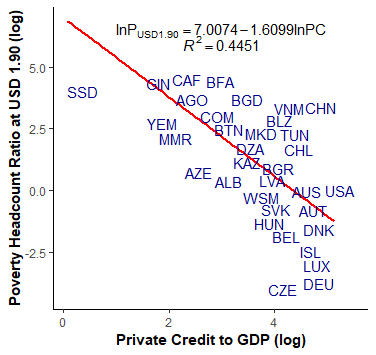
\includegraphics{190_PC}
\centering
\caption[Plot of Headcount Poverty at USD 1.90 against Private-sector Credit]{\textit{Negative relationship between log of poverty headcount (USD 1.90) and the log of private-sector credit to GDP. (Note: Based on data for 143 countries averaged over 1980-2015. Some country codes are omitted in order to increase legibility of the graph.)}}
\label{fig1}
\end{figure}

Fundamentally, a reduction in poverty either occurs through incrementing income or shifts in its distribution \cite{datt1992, bourguignon2003, klasen2008}. Thus, the main question raised within this paper is whether poverty reduction, as caused by mean income growth, better succeeds with higher degrees of financial development. To put it another way: does mean income growth better translate into decreasing poverty incidence in a sound financially developed environment? For the purpose of clarifying this issue, the paper examines whether the standard growth elasticity of poverty (GEP) equation as developed by \citeA{bourguignon2003} on the assumption of log-normally distributed incomes matches with financial development. This will be achieved by implementing an interactive term that conditions mean income growth on the level of financial development. The employed econometric models are specified by making use of three different poverty lines as dependent variables, namely the headcount ratios of USD 1.90, USD 3.20 and USD 5.50 a day. Such an approach yields the advantage that elasticities can be compared across poverty lines. Furthermore, the marginal effects of mean income growth can adequately be isolated for different income groups. An additional advantage is the comparability of the employed absolute poverty measures, both between and within countries. This is a major benefit which is withheld by relative indicators for poverty, such as the income share held by the lowest 20 percent.

Despite the apparent relevance of financial systems for further economic processes, there is disparity among scholars on how to adequately measure financial development. For instance, for the purpose of approximation, a multitude of empirical works either employs the ratio of money and quasi money (M2) or the already mentioned credit to the private-sector variable. Other authors have attempted to compute aggregate measures that aim to reflect the multidimensionality of the financial sector \cite<e.g.>{seven2016, svirydzenka2016, park2015}. This paper adopts such a measure for its main analysis alongside of the more common private credit variable. The employed measure\footnote{See Section (\ref{variables}) for a detailed description.} was developed by \citeA{svirydzenka2016} and properly incorporates the multidimensional nature of financial development. Certainly, every proxy for financial development will contain its drawback since it can only depict a small proportion of the true procedure happening in the financial economy. However, the application of both, a commonly used proxy and an aggregate variable that incorporates the multidimensionality of financial development, will serve as a focal point for comparison.

The paper utilizes unbalanced panel data for the period of 1980-2015 and for 63 countries.\footnote{See Table \ref{ObsByCountry} in Appendix \ref{SecObsByCountry} for a detailed list of usable country observations.} Data were averaged over five-year periods in order to eliminate business cycle fluctuations. Several estimation techniques are employed. First, pooled ordinary least squares (POLS) estimation is applied in order to explore the conditional relationship of mean income growth and financial development on poverty reduction. An additional estimation technique employed in this paper is represented by the fixed-effects estimator which, unlike POLS estimation, controls for country specific heterogeneity. The preferential estimations, however, stem from the exploited generalized method of moments (GMM) estimator. This is not least because of its ability to control for endogenous covariates, omitted variable bias and measurement errors.

This paper contains various contributions to the literature. Firstly, so far there has been no study that tested the conditionality of the standard GEP equation on financial development. Second, for this purpose the paper makes use of the recently developed financial development index by \citeA{svirydzenka2016} instead of solely depending on private-sector credit or other commonly used proxies. Furthermore, this paper adopts three different poverty headcount measures in order to identify idiosyncrasies of the different income groups that allow for comparability within and across countries. Updated data is utilized in order to calculate traditional elasticities of growth and poverty reduction. The study also attempts to find out whether there have been recent changes in the marginal effects of mean income growth on poverty alleviation conditioned on financial development. Finally, the study employs the system-GMM estimator on averaged data to control for endogeneity of the variables. According to present knowledge, the outlined procedure is unprecedented for GEP estimation.\footnote{GEP has been estimated by means of GMM estimation by e.g. \citeA{kalwij2007} and \citeA{fosu2017} but not for averaged data.}

The major findings of this paper are as follows: Poverty reduction caused by mean income growth is essentially supported by higher financial sector development. The marginal effects that mean income growth yields on poverty alleviation increase with higher levels of financial development. According to the employed data, this effect has even become stronger in recent periods. These results are robust to using different headcount poverty measures, financial development variables and estimation techniques. However, in a fully specified model that corresponds to the "Improved standard model 1" by \citeA{bourguignon2003} the effects of the financial sector development mechanism are absorbed when controlling for inequality and the inverse level of development. This indicates a joint relationship between financial sector, level of inequality and the degree of economic development. On the other hand, the interactions of changes in mean income and financial development, as well as their marginal effects, exert statistical significance in a standard equation where inequality and the inverse level of economic development are not included. This is especially the case when financial development is proxied by the compound index.

The paper is structured as follows. Section (\ref{review}) examines the literature on financial development and its effects on economic growth and poverty as well as the growth-poverty-inequality relationship. Data that was employed for this analysis will be explained in detail in Section (\ref{data}). Subsequently, the methodology will be demonstrated in Section (\ref{methodology}). Obtained results will be presented in Section (\ref{results}). Section (\ref{conclusion}) concludes.

\section{Literature review} \label{review}

The mere assumption that growth only will reduce poverty by any means seems to be no longer adequate. The "trickle-down" hypothesis appears to be obsolete and numerous scientists emphasized the significance of further factors that matter for the process of poverty reduction. Colonialism and institutional quality \shortcite<e.g.>{acemoglu2001}, geographic peculiarities \shortcite<e.g.>{bloom2003}, lack of insurance \cite<e.g.>{dercon2005}, to name but a few, were all brought into play as relevant factors for persisting poverty and/or absent economic growth. In the light of having achieved Millennium Development Goal (MDG) 1 of halving poverty by 2015, the international community proposed to itself the perhaps overambitious Sustainable Development Goal (SDG) 1 of exterminating poverty by 2030 \cite{UN2000, UN2015}. However, as outlined earlier in the text, poverty reduction rates experience recent stagnancy. Therefore, the identification of factors that foster economic prosperity for the deprived appears to be an urgent concern in order to achieve the set of goals that the international community has imposed on itself.

The relevance of financial markets for developing and middle-income countries was recognized by researchers and policymakers alike after the 1980s era, where a multitude of reforms established the beginning of market liberalizations worldwide. As will be discussed in the further course of this section, financial development is assumed to alleviate poverty by a large number of researchers. However, if this is the case, the level of financial development should play a role in determining the proportion of people leaving the area below the poverty line when mean income grows. Thus, a thorough examination of the literature is needed in order to shed light on existing gaps.

Since this paper aims to serve as a connecting piece between the poverty reduction, mean income growth and financial development strands of literature, considerable research from i) the growth-poverty-inequality nexus (see Section \ref{g-p-i}), ii) finance-growth nexus (see Section \ref{f-g}) and iii) the finance-poverty relationship (see Section \ref{f-g-p}) will be summarized hereafter. In the first instance, the macroeconomic relevance of financial systems will be briefly covered in the following subsection.

\subsection{Macroeconomic relevance of financial systems} 

Financial systems occupy a key position within the economic order. This is the main thrust contained in the extensive literature. In line with this, \citeA{stiglitz1993} awards the financial sector a role as the economy's "brain". More specifically, \citeA{merton1995} identify the areas of operations for the financial system as trade assistance, bundling of assets, risk management, overcoming information asymmetries, provision of price information and the relocation of assets through borders, time and businesses. Furthermore, \citeA{seven2016} observe that the main functions of financial systems in the economic order consist of the enhanced allocation and formation of capital and the mobilization of savings. \citeA{saunders1997} detect that for settings without financial intermediaries, poor communication between firms and individuals concerning the exchange of funds predominates. Moreover, \shortciteA{johnston2000} state that financial intermediaries emerge due to existing information asymmetries. On the other hand, \citeA{allen1997, allen2001} attribute financial intermediaries the role of risk transferrers and guides through the incremental complexity of the financial system. The authors criticize that the view on financial intermediaries as transaction cost and asymmetric information reducers is outdated and too strong.

Furthermore, scholars increasingly accept the assumption of growth promotion and poverty reduction by properly functioning financial sectors. This is mainly justified by efficiency gains that lower the cost of information and transactions \cite{king1993, bencivenga1995, beck2004a}. The evidence on this view will be examined in the following sections.


\subsection{Finance-growth nexus} \label{f-g}

The relevance of the financial sector for economic prosperity has been occupying economists' minds for some time. A growth promoting financial sector was already proposed by \citeA{goldsmith1969}, \citeA{mckinnon1973} and \citeA{shaw1973}. Despite their findings, further research on the finance-growth relationship was mainly suspended for the following two decades. Subsequently, it was thanks to the occurrence of endogenous growth models that economists rediscovered their enthusiasm for the finance-growth strand of literature \cite{pagano1993}. In his thorough examination of a large number of empirical and theoretical works on the relationship between finance and growth, \citeA{levine2005} concludes that certainly there is some association between economic improvement and a well-performing financial sector in the long run.

In their theoretical framework, \citeA{greenwood1990} model that financial development plays a key role for economic development by allowing for rising returns on capital investment which in turn help incomes to increase. \citeA{pagano1993} identifies three channels through which financial development can impact economic growth: the transmission of private savings to firms (i), the enhancement of capital allocation (ii) and its impact on the economy's overall savings rate (iii). In another endogenous growth model, \citeA{levine1991} establishes a link between stock markets and stimulated economic growth through the offering of possibilities for diverse portfolios and the improvement of stock broking without interfering in firms' production processes.

Supplementary to theoretical modelling approaches, there have been considerable empirical cross-country studies on the finance-growth relationship. By using a panel of 40 countries, \citeA{beck2004a} investigate the interconnection of bank development, stock markets and economic growth. They conclude that finance has an affirmative influence on overall economic development and thus reject theories that attribute a negative or miniscule role to the financial sector. The results by \citeA{beck2004a} are later confirmed by \citeA{khadraoui2012} who empirically tested finance's positive impact on growth by constructing a panel dataset of 70 both developing and developed countries. However, the latter likewise criticize the lack of expressiveness for available proxies in the measurement of financial development. By using a semiparametric approach as an aid, \citeA{herwartz2014} find evidence for a more powerful effect of finance on growth in high-income countries. According to the authors, this impact possibly depends on government size, since a reverse effect can occur in cases where governments are significantly involved in the economy.

Other authors are in favor of a small-scale examination of the finance-growth nexus. Rather than conducting cross-country studies, \citeA{ram1999} stresses the importance of looking into individual country cases when evaluating the impact of financial development on economic growth. In an effort to identify key shortcomings for African development, \citeA{easterly1997} find one of the reasons for Africa's low growth rates in lower levels of financial development. In a time series study for India covering the period 1970–1971 to 1998–1999, \citeA{bhattacharya2003} conclude that financial development causally influences GDP growth, thereby excluding the possibility for the reverse direction.

Apparently, evidence for growth encouraging financial development is abundant. Thus, a relatively recent strand of literature is concerned with a slowing or rather negative impact that financial development wields on economic growth, once it reaches a peak. On that note, \citeA{rousseau2011} find that the growth promoting effect that was exerted by financial development for data for the 1960s and 1980s is no longer present for more recent data. The authors argue that exorbitant growth rates of bank credit lending supposedly worsened banking systems and cleared paths for financial crises that harmed overall economic growth. \citeA{law2014} identify a threshold up to which financial development promotes economic growth. The authors argue that once the threshold is reached, further financial development would negatively impact the prosperity of an economy. Therefore, they conclude that a more favorable level of financial development below the threshold should be targeted by policymakers. Similarly, \shortciteA{arcand2015} examine such a threshold in a much-noticed study. They determine that private-sector credit beyond 100 percent of GDP exhibits adverse effects on economic growth. As possible reasons for such an effect, \shortciteA{arcand2015} provide the lowering importance of credit markets as economies develop, the augmented risk for financial crises and a reallocation of the labor force from productive sectors to the financial sector (brain drain).

This thesis will also take into account the suggested declining effect of financial development and extend the hypothesis to poverty reduction. This will be achieved by exclusion of data that covers more recent periods and the comparison of results for different time spans. In this manner, it is intended to detect whether the translation of income growth to poverty reduction has declined over time. However, instead of solely depending on a single measure of financial development, the analysis will employ one compound variable and private-sector credit.

As outlined in this section, the evidence on a strong relationship between growth and finance is abundant. Further research has widened the focus of analysis and extended the viewpoint towards a joint relationship between finance, growth and poverty. Considerable studies will be presented in the following section.


\subsection{Finance-growth-poverty nexus} \label{f-g-p}

The previous section presented a series of nameable investigations that examine the relationship between finance and growth. This section deals with the extension of that relationship to the connection of finance, growth and poverty.

As theory suggests, poverty alleviation and financial development are closely linked through the provision of better access to services by the financial sector. Moreover, the poor can access credit and insurance assistance by means of improved financial markets. Thus, sustenance and productivity of the poor can be reinforced substantially \cite{jalilian2002}. However, in the comprehensive literature results are mixed. \citeA{jalilian2002, jalilian2005} observe a link for the finance-growth-poverty relationship and an additional threshold of economic development up to which financial development influences diminishing poverty incidence by the promotion of growth. By using three-stage least squares on a panel with 132 countries containing observations from 1980 to 2014, \shortciteA{kaidi2019} assess the relationship of financial development, institutional quality and poverty. They, on the other hand, report no significance for possible effects that financial development has on poverty reduction. \citeA{naceur2016} divide financial development into five dimensions and separately test the effect of each aspect on changes of income distribution and poverty incidence. Their results, in turn, suggest that every dimension of financial development except for financial liberalization reduces poverty and inequality.  \citeA{akhter2009} identify financial instability as a harmful factor for poverty reduction. In their analysis, the authors undertake a separation of direct and indirect\footnote{\citeA{akhter2009} argue that prior studies had only focussed on the indirect effect of financial development on poverty reduction through economic growth. They recognize direct effects through boosts in the ratio of credits to the private sector and liquid assets of the financial system (M3), both as a share of GDP.} effects of financial development on changes of poverty. The authors conclude that improved possibilities of saving and borrowing are beneficial to diminishing poverty rates. \citeA{jeanneney2011} also distinguish between financial development that affects poverty by a direct and indirect channel. Their results suggest that the direct effects outweigh the indirect impacts and plead for the McKinnon conduit effect as the main cause of accelerated poverty reduction. \citeA{boukhatem2016} finds a direct contribution of financial development to poverty alleviation but admonishes of the devastating effects that financial instability has for the poor. In a more recent effort, \citeA{rewilak2017} reclaims negative impacts of financial instability on poverty rates and provides additional evidence for poverty alleviation by financial deepening and physical access to financial services.


As mentioned previously, it is important to note that there is no agreement among scholars on how to adequately measure financial development. Hence, there is a wide range of variables that serve as approximations. Widely used proxies include, for example, the already presented private-sector credit variable or some liquidity measure, such as M2 or the broader currency plus demand and interest-bearing liabilities of banks and non banks (M3) \cite<e.g.>{perez2011}. Apart from this, \citeA{dollar2002} utilize commercial bank assets divided by total bank assets as a financial development proxy and observe the measure to have an impact on income growth with negligible effects on its distribution. The authors therefore conclude that policies which aim for the promotion of financial development are helpful for the success in poverty alleviation. Other authors advocate the private-sector credit measure. This variable was introduced to the finance-poverty literature by \shortciteA{beck2004b}, who certify the measure pro-poor growth qualities. In a later attempt, the authors ascertain that financial development, once again measured by private credit, significantly helps in lowering the proportion of people living on below USD 1 a day \shortcite{beck2007}. Equally, \citeA{honohan2004} notes poverty reducing effects that stem from private credit. On the contrary, \citeA{perez2011} does not find any causal relationship from private credit to poverty. However, for M2 and M3 as proxies for financial development, \citeA{perez2011} detects a causal relationship that holds only for the 1970s and 1980s. More recently, \citeA{rewilak2017} proxies access to finance by the number of ATMs per 1000 $km^{2}$ and the number of bank branches per 1000 $km^{2}$. This paper also makes use of private-sector credit along with a compound variable which attempts to adequately reflect the multidimensionality of the financial sector. Although innovative measures such as the number of ATMs and bank branches are interesting considerations for an adequate depiction of financial development, they suffer from short time series and result in lower observation counts. Therefore, this study opts for higher data availability and does not include such measures.


Apart from measurement issues for financial development, a country's state of economic development or its geographical position have played a role in the consideration for analysis of the finance-growth-poverty nexus. Thus, several authors have restricted their analyses to only middle-income countries. One such examination has been conducted by \citeA{seven2016} for a panel consisting of 45 countries with observations ranging from 1987 to 2011. The authors find growth fostering but no significant poverty reducing effects in financial development. Analogously, neither do \shortciteA{kaidi2018} identify poverty alleviating properties for financial development in middle-income countries.\footnote{Notably, the scholars find stock market enhancement to be beneficial to the poor.} \citeA{park2015} focus their analysis on 37 Asian countries and test the impact that financial inclusion has on levels of poverty and inequality. Their results indicate that both, income inequality and poverty are scaled down by financial inclusion. In a subsequent study, \citeA{park2018} extend their analysis on a sample of 176 countries from all world regions and find significant correlations for financial inclusion and lower poverty incidence and a more egalitarian income distribution. In contrast to the presented studies, this paper does not impose any geographical restrictions on the analysis. The sample covers low- and middle-income countries of all regions. This is due to the fact that poverty constitutes a supra-regional constraint and is salient especially for countries that are classified as low-income.

Furthermore, a large body of literature laid the focus on the country-level. While such an approach will most probably lack general validity, it nevertheless yields the advantage of thoroughly investigating a specific country's case. In their time-series analysis for Nigeria between 1980 and 2010, \citeA{dauda2014} find financial deepening measured in terms of M2 to be poverty reducing. On the contrary, in the same analysis credit to private sector exacerbates the incidence of poverty. The authors explain this particular finding by pointing to the failure of financial intermediaries to provide the poor with sufficient savings tools. Similarly, \citeA{quartey2008} criticizes Ghanaian financial players for not having efficiently allocated savings possibilities to areas of business that benefit the poor. For the case of Bangladesh, \shortciteA{uddin2014} concede a non-linear poverty reducing effect to a properly functioning financial sector. \citeA{odhiambo2009} compares South African real and financial sectors in order to detect which of the two has a stronger influence on the reduction of poverty. The author concludes that both sectors are helpful for escaping poverty in the South African case. With quarterly data on Egypt covering the period of 1975-2011, \shortciteA{abosedra2016} identify a long-run interconnection between growth, financial deepening and poverty reduction. Nonetheless, their results mainly depend on the choice of proxies for financial development. This is in line with several findings in the finance-growth-poverty literature.

To sum up, results for the analysis of the finance-growth-poverty nexus leave space for ambiguities. While a variety of studies finds financial development to be poverty reducing, results seem to be dependent on the employed measure. Therefore, it is important to make use of a broader measure that takes into account the plurality of financial sectors. This paper tries to overcome the problems associated with imprecise proxies by utilizing a compound measure developed by \citeA{svirydzenka2016}. The variable is discussed in depth in Section (\ref{variables}). The study furthermore distinguishes the direct and indirect effects of financial development by taking into account marginal effects of income growth on the reduction rate of poverty at different stages of financial development. The theoretical framework for this consideration stems from literature on the growth-poverty-inequality nexus which is described in the next section.


\subsection{Growth-poverty-inequality nexus} \label{g-p-i}

Economic growth might not always reach the poor. Awareness for such an unfavorable circumstance has caused extensive reflections regarding the concept of "pro-poor growth". With the rise of this term, a multitude of scholars became increasingly interested in how much economic growth translates into poverty reduction. However, a proper definition of the notion has been subject to a lot of dispute. Some authors view growth as pro-poor if incomes of the poor rise at a higher pace than the livelihoods of the well-off \cite{baulch2000, kakwani2000}. Proponents of the alternative, more 'generous', view define growth as pro-poor if the poverty measure of interest drops at the presence of income growth \cite{ravallion2003}.

In their landmark paper, \citeA{dollar2002} lay the foundation for an ever-growing body of literature related to the pro-poor features of mean income growth. The authors examine overall mean income growth rates and the average income growth rates of the poor\footnote{\citeA{dollar2002} use the lowest quintile of the income distribution in order to measure poverty.}. \citeA{dollar2002} find that these growth rates do not substantially differ and therefore conclude that economic growth equally benefits the poor as well as the wealthy. Building on their previous research, \citeA{kraay2006} employs decomposition techniques on growth rates of poverty and concludes that high average income growth and a change in relative incomes are in line for potential causes of pro-poor growth.

 In a much-noticed cross-country study, \citeA{bourguignon2003} assumes log-normality for the distribution of mean income and is thus able to calculate an identity for poverty reduction, changes in inequality and growth of mean income. Prior to the log-normality assumption by \citeA{bourguignon2003}, studies on the GEP usually focussed on single country cases\footnote{For comparable GEP studies that take into account the poverty-inequality-income identity on the country level see for example \citeA{ravallion1991}, \citeA{datt1992}, \citeA{kakwani1993} and \shortciteA{kakwani2000}.}, since knowledge on the complete distributional qualities of incomes on the household level is imperative \cite{klasen2008}.
 
 On a more general note, \citeA{ram2006} advises caution with regard to GEP estimates being too high to be realistic. Heterogeneity among the GEP estimates is indeed very common. While some authors find GEP to lie between -2.0 and -3.0 \cite<e.g.>{ravallion1999}, others report estimates to be as high as -5.0 or even higher \cite<e.g.>{bhalla2002, bourguignon2003, fosu2017}. \citeA{adams2004}, for example, contests the GEP estimates suggested by \citeA{bhalla2002}. The first-mentioned author furthermore stresses the divergence of estimates for differing proxies of economic growth, namely the growth rate of survey mean income and changes in GDP per capita. By investigating a panel of 58 developing countries for the period 1980-1998, \citeA{kalwij2007} show that the large variation in GEP across regions can be mostly explained by differences in initial inequality levels. In an analogous endeavor, \citeA{fosu2009} examines the dimension in which levels of inequality influence the translation of mean income growth into poverty reduction. He compares countries in sub-Saharan Africa to other regions. The author concludes that there is large variation in GEP, even among countries of the same region. However, GEP is considerably less for countries in sub-Saharan Africa \cite{fosu2009}. These findings are then confirmed by \citeA{fosu2017} for updated data from the 1990s onwards, a period in which developing countries experienced high rates of mean income growth.\footnote{Interestingly enough, \citeA{fosu2017} finds that a majority of countries registered declining poverty rates for the observed time span. However, according to the author, almost all of this reduction stems from mean income growth rather than changes in inequality levels.} \citeA{lenagala2010} note diminishing GEP over time and extensive differences in GEP for the distinct poverty lines that they employ. Furthermore, they reinforce \citeA{ram2006} by stating that most GEP estimations tend to be unrealistically high.

In a recent hybrid study covering data on 90 developing countries and on regions in Rwanda and Ethiopia, \shortciteA{ouyang2018} investigate whether the pace of poverty reduction is dependent on reduced initial poverty incidence. The authors confirm their hypothesis that lower initial poverty leads to its faster consecutive reduction for all observed units. Furthermore, they find that SSA countries, contrary to others, tend to grow faster if initial poverty incidence is high. Another recent study by \shortciteA{khan2019} finds that GEP depends on the colonial history of African countries. According to the authors, GEP is higher in former smallholder economies. The scholars attribute this circumstance to a more egalitarian income distribution in such countries.

This study serves as a connecting piece for all presented strands of literature in this section. Poverty reduction will be treated as a complex interplay between growth, inequality and financial development. The paper takes into account all these concerns and relates them in a coherent context. Achieving this objective involves the selection of variables and the construction of an adequate dataset. These issues will be addressed in the next section.

\section{Data} \label{data}

The main focus of this paper is on testing the conditional relationship that income growth and financial development jointly exert on changes in poverty. Therefore, adequate measures for important determinants such as poverty, inequality, financial development and income are needed in order to construct the basis for the intended analysis. This section deals with the explanation of variables and their sources. Moreover, it will provide summary statistics. First of all, the next segment describes the constructed sample. 

\subsection{Sample}

The sample involves low- and middle-income countries and excludes those countries that are classified as high-income. The reasons for this strategy are threefold. Firstly, results would be biased due to low realizations in poverty headcount measures for high-income countries. Second, sample heterogeneity can be lowered by focusing on a more comparable set of economies. Finally, high-income economies tend to have higher developed and more diversified financial sectors where commonly used proxies such as private-sector credit are unable to provide full apprehension.

The dataset comprises 63 countries\footnote{See Appendix \ref{CountryList} for a detailed list of countries.} for the period of 1980-2015. This period grants special insights on all utilized indicators for the selected list of countries. In particular, data on mean income and income distribution are only available from the 1980s onwards. Nonetheless, severe challenges consisting of data limitations were faced during the construction of the dataset. This is due to the reason that for many low- and middle-income countries frequent statistics are available only from the late 1990s onwards. Hence, data were averaged over seven non-overlapping five-year periods\footnote{The seven periods consist of the following five-year sequences: 1980-1984 (1), 1985-1989 (2), 1990-1994 (3), 1995-1999 (4), 2000-2004 (5), 2005-2009 (6), 2010-2015 (7) with the most recent period covering six years.} in order to eliminate short term fluctuations and tackle missing data problems.\footnote{\citeA{khadraoui2012} note that averaging data has become a favored method in dynamic panel models in order to allow for rolling panel data.} Averaging the data can furthermore be justified by the implementation of the system-GMM estimator, as it demands fewer time points and an increased number of cross-sections \cite{seven2016}. Moreover, gapless time series observations were prioritized. Only those countries with five or more observations for the entire time span were included, accordingly. Furthermore, countries were restricted to those that had two or more consecutive observations in the averaged dataset. Missing values between two periods were interpolated in order to be able to include as many countries as possible. For those cases where a country's headcount decreases to 0 over time, values were approximated to 0.001 in order to be able to take logarithms.\footnote{The following approximations were undertaken: Jordan (1985-1989), Belarus (2010-2015), Argentina (1985-1989), Ukraine (2010-2015), Bulgaria (1990-1994), Azerbaijan (2005-2009) for the USD 1.90 headcount as well as Bulgaria (1990-1994) and Azerbaijan (2005-2009) for the USD 3.20 line. See \citeA{fosu2017} for a comparable  strategy.}

In this paper, growth rates are generally computed as logarithmic differences divided by the number of years. A notable exception is growth rate of population since it was available as such. Unfortunately, the dataset further reduces by calculating growth rates since the change from two consecutive periods can only be expressed in a single number. Thus, the estimations for the main analysis contain between 270 and 268 observations.

\subsection{Variable description} \label{variables}

For the econometric analysis, key variables were selected with respect to their availability and expressiveness. Furthermore, the variables largely correspond to commonly used measures in the literature. A thorough description of the variables and their sources will be provided in this section.

The poverty headcount ratios at USD 1.90, USD 3.20 and USD 5.50 a day expressed in 2011 Purchasing Power Parity (PPP) capture the percentage share of a population that lives in households with income or consumption below the respective poverty line. The growth rates of these variables are treated as dependent variables in the estimations. They can be compared both across and within countries and thus represent adequate measures for this investigation. This comparability creates a major advantage that headcount ratios have over relative poverty measures such as the income share held by the lowest 20 percent. The income measure employed in this study is the average monthly per capita income or consumption expenditure in a household and is expressed in 2011 PPP USD. The variable is based on survey data, comparable to the headcount ratios.

In addition, an adequate measure for income inequality is required. The Gini index measures income inequality and takes a value between 0 (perfect equality) and 100 (perfect inequality). All of the above mentioned variables were retrieved from PovcalNet\footnote{\url{http://iresearch.worldbank.org/PovcalNet/povOnDemand.aspx}}. The only exception is population growth rate which was obtained from World Bank's World Development Indicators\footnote{\url{https://data.worldbank.org/}}.

Furthermore, adequate indicators for financial development are needed for the analysis. It is with this aim in view that this paper utilizes two different proxies for comparison purposes. Private-sector credit to GDP is a commonly used proxy for financial development in both, the finance-growth and the finance-growth-poverty literature strands. In particular, it measures the credit share of financial intermediaries to the private sector, thereby excluding credit to public institutions. As already mentioned above, several authors have emphasized the qualities of this measure in serving as an indicator for financial development \shortcite<e.g.>{beck2004b, honohan2004, beck2000}. Private-sector credit is retrieved from the Global Financial Development Database\footnote{\url{https://www.worldbank.org/en/publication/gfdr/data/global-financial-development-database}}. A growing body of literature stresses the inability of the private credit measure to depict the complexity of the financial sector \cite<e.g.>{seven2016, svirydzenka2016}. Moreover, in modern days financial systems became more versatile. Hence, they involve more players that go beyond the scope of mere banks. Therefore, this study employs another variable that attempts to measure the degree of financial development. The Financial Development index (FD index) was developed by \citeA{svirydzenka2016} and was retrieved from IMF Data\footnote{\url{http://data.imf.org/?sk=F8032E80-B36C-43B1-AC26-493C5B1CD33B}}. This measure combines financial institutions and financial markets, as well as their respective sub-dimensions. These three dimensions consist of depth, access and efficiency. Eventhough the FD index is a major improvement towards a more suitable depiction of financial development, some of its drawbacks are the lack of inclusion of possible legal, institutional and regulatory structures as well as thereby resulting financial instability. The construction of the index takes place in three steps in order to reduce and incorporate the multidimensional data into one final measure. First, the multifaceted measures are normalized. As a next step, sub-indices for each dimension are fed with the data. Lastly, the final index is created by assembling all sub-indices in the FD index \cite{svirydzenka2016}.

By way of comparison to Figure (\ref{fig1}), Figure (\ref{fig2}) plots the relationship of FD index with the headcount ratio of USD 1.90 a day. It becomes clear that, just as private-sector credit, the FD index is associated with a lower poverty headcount.

\begin{figure}[h]
	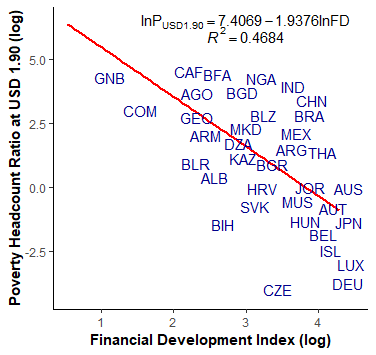
\includegraphics{190_FD}
	\centering
	\caption[Plot of Headcount Poverty at USD 1.90 against the FD index]{\textit{Negative relationship between log of poverty headcount (USD 1.90) and the log of the Financial Development Index by Svirydzenka (2016). (Note: Based on data for 143 countries averaged over 1980-2015. Some country codes are omitted in order to increase legibility of the graph.)}}
	\label{fig2}
\end{figure}

\subsection{Summary statistics}

Table \ref{tab:summary} reports summary statistics for the constructed sample.\footnote{See Appendix \ref{MainVarsCountry} for a list of main variables for each country.} Large variations can be observed for all employed poverty headcount measures. For example, in Bulgaria 0.7 percent of the population lived on less than USD 5.50 a day in the 1990-1994 period. At the further end, 98.3 percent of the population lived below that same threshold in Niger during the same period. The same magnitude of variation applies to the distribution of mean income. While Guinea had the lowest observed mean income in 1985-1989 with 23.88 USD PPP, the realization for Georgia for 1980-1984 is the highest in the sample with 893.77 USD PPP.

\begin{table}[ht]
	\centering
	\begin{tabular}{lrrrrr}
		\toprule
		Variable & \multicolumn{1}{c}{Obs} & \multicolumn{1}{c}{Mean} & \multicolumn{1}{c}{Std. Dev.} & \multicolumn{1}{c}{Min} & \multicolumn{1}{c}{Max} \\
		\midrule
		Poverty headcount ratio at USD 1.90 & 333   & 21.638 & 22.059 & 0.001 & 83.100 \\
		Poverty headcount ratio at USD 3.20 & 333   & 39.774 & 28.716 & 0.001 & 93.850 \\
		Poverty headcount ratio at USD 5.50 & 333   & 60.019 & 27.839 & 0.700 & 98.300 \\
		Gini index & 332   & 42.328 & 8.731 & 24.540 & 63.900 \\
		Mean income in USD & 441   & 228.488 & 153.489 & 23.869 & 893.768 \\
		Private-sector credit to GDP & 403   & 29.805 & 25.879 & 0.273 & 145.302 \\
		FD index & 411   & 21.077 & 11.972 & 0.003 & 66.068 \\
		\bottomrule
	\end{tabular}
	\caption[Summary Statistics]{\textit{Summary statistics}}
	\label{tab:summary}
\end{table}%

The included proxies for financial development are also subject to considerable variation. Private-sector credit to GDP ranges from 0.27 percent in Lao PDR in 1985-1989 to 145.30 percent in Thailand in 1995-1999. The FD index has its lowest realization for the Russian Federation in 1980-1984. The highest observation, in turn, is reported for Malaysia with 66.07 percent in 2010-2015.

Table \ref{tab:Corr} displays correlations for key variables that will enter the later regression analysis conditional on mean income growth. The table allows for interesting insights as it indicates that the covariates include reciprocal information. Indeed, FD index and private credit never enter the same specification as they serve as placeholders for financial development. However, the ratio of poverty line over mean income, $(Z_{x}/Y_{it})$, is negatively correlated with both finance indicators and the Gini index. This downhill correlation is somewhat weak with FD index and the Gini coefficient (-0.2372 and -0.2996) and at a moderate level with private-sector credit (-0.4519). Correlations of this form may result in multicollinearity and further problems associated with overparameterization \cite{seven2016}. These concerns will be discussed in depth in the following sections.

\begin{table}[hb]
	\centering
	\begin{threeparttable}
		{
			\begin{tabular}{lcccc}
				\toprule
				& \multicolumn{1}{c}{$FD\,Index$} & \multicolumn{1}{c}{$Private\,Credit$} & \multicolumn{1}{c}{$Gini$} & \multicolumn{1}{c}{$(Z_{x}/Y_{it})$} \\
				\midrule
				$FD\,Index$ & 1     &       &       &  \\
				$Private\,Credit$ & 0.7074 & 1     &       &  \\
				$Gini$  & 0.0678 & 0.1916 & 1     &  \\
				$(Z_{x}/Y_{it})$ & -0.2372 & -0.4519 & -0.2996 & 1 \\
				\bottomrule
			\end{tabular}%
		}
		\begin{tablenotes}
			\item{Note: All variables are expressed in natural logarithms.}
		\end{tablenotes}
	\end{threeparttable}
		\caption[Correlation Matrix for Covariates]{\textit{Correlation matrix}}
		\label{tab:Corr}%
	\end{table}%


This section provided a thorough description of the constructed dataset. Additionally, sources for the data were provided and summary statistics were presented. The next section outlines the theoretical foundation and empirical strategy on which this paper is based.

\newpage
\section{Empirical methodology} \label{methodology}

The preceding sections provided a thorough literature review as well as a detailed description of the dataset. In the extensive literature on changes in poverty, mean income growth has been pointed out to be the main driver for poverty alleviation. Following the hypothesis underlying this paper, the level of financial development should play an important role in the translation of mean income growth into poverty reduction. In order to determine the truthfulness of this assumption, a competent estimation strategy is required. The first part of this section lays the theoretical foundation for the econometric model. Subsequently, the estimation framework is explained in greater detail.

\subsection{Model}

For the purpose of inspecting the effects of mean income growth on poverty reduction with varying levels of financial development, a standard GEP model is needed. The GEP specification described in this section is closely oriented by \citeA{bourguignon2003}, \citeA{epaulard2003}, \citeA{kalwij2007} and \citeA{fosu2009} who assume a lognormal distribution of income. Furthermore, the aforementioned works include the ratio of the poverty line to mean income and initial inequality as independent factors by which GEP is influenced. The model of interest is written as

\begin{equation} \label{eq:1}
p_{x,it} = b_{1} + b_{2}y_{it} + b_{3}g_{it} + b_{4}(Z_{x}/Y_{it}) + b_{5}G_{it-1} + b_{6}y_{it}\times G_{it-1} + b_{7}y_{it}\times (Z_{x}/Y_{it})
\end{equation}

where $p_{x,it}$ is the change in the respective poverty rate in country $i$ at time period $t$, $y_{it}$ is the growth rate of mean income, $g_{it}$ is the growth rate of the Gini coefficient, $G_{it-1}$ is the initial inequality as measured by the Gini coefficient and $(Z_{x}/Y_{it})$ is poverty line $Z$ divided by mean income $Y_{it}$\footnote{For instance, in the case of the USD 1.90 poverty line, the inverse level of development, $(Z_{1.90}/Y_{it})$, is calculated as follows: $Z = 1.90 \times \frac{365}{12}$. In this manner, the poverty line of USD 1.90 a day is expressed on a monthly basis since mean income $Y_{it}$ is also given as such. The obtained value of $Z$ is then divided by $Y_{it}$, thus resulting in the ratio of the poverty line to mean income per month. Note that this procedure is done for all three deployed poverty lines accordingly.}. The interaction terms that include initial Gini and the ratio of poverty line over mean income jointly serve as approximations for population density in vicinity of the poverty line \cite{kalwij2007}.

The inverse of the level of development, $(Z_{x}/Y_{it})$, together with the level of inequality, $G_{it}$, play a decisive role in GEP modelling. $(Z_{x}/Y_{it})$ measures how far apart mean income and poverty line are from each other, i.e. the size of mean income $Y_{it}$ relative to the poverty line $Z_{x}$. According to \citeA{bourguignon2003}, GEP is an increasing function of the level of development but a decreasing function of the level of inequality. A higher inverse of the level of development would mean that either the poverty line is set very high or that mean income is relatively low. Therefore, one can expect an effect that would decrease overall GEP.

At this point, it must be noted that the constitutive terms consisting of $G_{it-1}$ and $(Z_{x}/Y_{it})$ tend to be omitted from Equation (\ref{eq:1}) without the provision of an explanation for this strategy \cite<see e.g.>{bourguignon2003, fosu2009}. However, constitutive terms, even if statistically insignificant, should be included in such specifications since their omission may lead to misleading interpretations and deficient analyses due to occurring biased estimates \shortcite{golder2006, brambor2007, golder2012}. In order to prevent such issues, the analysis for this paper will add all constitutive terms to specifications where their interactions are also imposed.


This paper argues that the relationship depicted in Equation (\ref{eq:1}) should further include financial development as an important driver behind changes in headcount poverty. The reasons for the inclusion of this additional term are obvious. Financial development grants poor households better access to services provided by the financial sector. These services can consist of improved payment methods, enabling of savings possibilities, affordability of credit and access to insurance. These channels can help households in escaping poverty through lower transaction costs, better risk management, facilitated investment possibilities and diminished income volatilities \cite{claessens2007}. Thus, the empirical model that is employed in this paper extends Equation (\ref{eq:1}) and includes the level of financial development interacted with mean income growth:

\begin{equation} \label{eq:2}
\begin{split}
p_{x,it} ={} 	& b_{1} + b_{2}y_{it} + b_{3}g_{it} + b_{4}(Z_{x}/Y_{it}) + b_{5}G_{it-1} + b_{6}y_{it}\times G_{it-1} \\&+ b_{7}y_{it}\times (Z_{x}/Y_{it}) + b_{8}FD_{it} + b_{9}y_{it}\times FD_{it}
\end{split}
\end{equation}
where $FD_{it}$ denotes financial development in country $i$ at time period $t$. In this paper, Equation (\ref{eq:2}) will be treated as the fully specified model.

As a next step, it is important to determine the expected signs of the parameters in Equation (\ref{eq:2}). These will be discussed hereafter. The sign of $b_{2}$ is expected to be negative, because increasing mean income is supposed to decrease poverty at a faster pace, ceteris paribus. On the contrary, $b_{3}$ is expected to exert a positive effect on the poverty growth rate since poverty will exacerbate with higher rates of inequality growth. The sign of $b_{4}$ is anticipated to be one of the causes for a rising poverty headcount. A similar consideration can be applied to $b_{5}$, since higher initial inequality can be expected to have increased poverty. For both, $b_{6}$ and $b_{7}$, a positive sign can be anticipated since higher initial inequality and an increased ratio $(Z_{x}/Y_{it})$ would enter as inhibiting factors for the translation of mean income growth into poverty reduction \cite{fosu2009}. In accordance with a large number of studies that were described in section (\ref{f-g-p}), in this paper financial development is assumed to account for faster poverty alleviation. Therefore, the signs of both, $b_{8}$ and $b_{9}$, are expected to be negative. This is backed by the assumption that higher developed financial systems ease access to finance and therefore also help in better translating mean income growth into poverty reduction.

Nonetheless, there are a few concerns regarding the included paramaters in Equation (\ref{eq:2}). Financial development is known to affect inequality and the level of economic development \cite<e.g.>{beck2004b, beck2007, seven2016}. The correlations of respective indicators in the employed dataset can be seen in Table \ref{tab:Corr}. The two parameters for inequality and inverse level of economic development, depicted by $G_{it}$ and $(Z_{x}/Y_{it})$ in Equation (\ref{eq:2}), might possibly absorb the effect of financial development on changes in poverty. Thus, the finance parameter might suffer from the addition of inequality and inverse level of development variables in the later econometric specification.


As a next step, the derivation of marginal effects will be outlined. since these are the key to an adequate interpretation of interactive models. For reasons of simplicity and for the purpose of deducting marginal effects from the interaction of mean income growth and the level of financial development, a more straightforward specification than equation (\ref{eq:2}) is required. Following \citeA{bourguignon2003}, a standard model version of equation (\ref{eq:2}) can be written as:

\begin{equation} \label{eq:3}
p_{x,it} = b_{1} + b_{2}y_{it} + b_{3}g_{it} + b_{8}FD_{it} + b_{9}y_{it}\times FD_{it}.
\end{equation}

Equation (\ref{eq:3}) attributes changes in poverty to an intercept $b_{1}$, the independent effect of $y_{it}$ (when $FD_{it} = 0$, i.e. in the absence of financial development in country $i$ at time period $t$), the effect of $g_{it}$, the independent effect of $FD_{it}$ (when $y_{it} = 0$) and the interaction of $y_{it}$ and $FD_{it}$. For this model, the marginal effect (ME) of $y_{it}$ on $p_{it}$ is denoted by:

\begin{equation} \label{eq:4}
ME(y_{it}|FD_{it}) = \frac{\partial p_{it}}{\partial y_{it}} = b_{2} + b_{9}FD_{it}
\end{equation}

For equation (\ref{eq:4}), the marginal effect of mean income growth $y_{it}$ on the rate of poverty reduction $p_{it}$ is conditional on the level of financial development $FD_{it}$ (unless $b_{9}$ is zero). Due to the fact that equation (\ref{eq:3}) contains an interactive term of symmetric nature, the marginal effect of $FD_{it}$ on $p_{it}$ is furthermore conditional on $y_{it}$, thus resulting in

\begin{equation} \label{eq:5}
ME(FD_{it}|y_{it}) = \frac{\partial p_{it}}{\partial FD_{it}} = b_{8} + b_{9}y_{it}.
\end{equation}

In this manner, the coefficient of the interacted term, $b_{9}$, expresses the slope for $ME(y_{it}|FD_{it})$ and $FD_{it}$ connection, as well as the slope for the relationship between $ME(FD_{it}|y_{it})$ and $y_{it}$. Therefore, it is consequently assumed that the marginal effect of mean income growth on the poverty growth rate is negative for any level of financial development higher than zero. In the same way, the marginal effect of financial development from (\ref{eq:5}) is expected to yield a negative marginal effect on the growth rate of poverty, as long as mean income growth is positive.

This section has described the theoretical model that is employed in this paper. In detail, it has derived the main marginal effects formulation of interest, which is described in Equation (\ref{eq:4}). The aim is now on merging the theoretical groundwork with an adequate estimation strategy. The next section describes the underlying empirical framework in greater detail.


\subsection{Estimation framework}

This paper argues that, with higher levels of financial development, mean income growth performs better in the process of poverty reduction. In the preceding section, an adequate theoretical basis for the underlying hypothesis of this paper has been laid. The examination of the hypothesis furthermore requires a competent empirical strategy that exploits the advantages and overcomes the shortcomings of the dataset described in Section (\ref{data}). Due to the panel structure of the employed data, unobserved country specific characteristics can be controlled for. This is a major advantage that this study has over cross-sectional studies. This section furthermore discusses the applied estimation techniques together with their advantages and drawbacks.

The fully specified econometric model that is employed in this paper is a multiplicative interaction model derived from Equation (\ref{eq:2}). It reads as follows:

\begin{equation} \label{eq:6}
\begin{split}
\Delta \, logPoverty_{x,it} ={} 	& \beta_{1} + \beta_{2} \, \Delta \, logMeanIncome_{it} + \beta_{3} \, \Delta \, logGini_{it} + \beta_{4} \, log(Z_{x}/Y_{it})  \\ &+ \beta_{5} \, logGini_{it-1} 
+ \beta_{6} \, \Delta \, logMeanIncome_{it}\times logGini_{it-1} \\ &+ \beta_{7} \, \Delta \, logMeanIncome_{it}\times log(Z_{x}/Y_{it}) + \beta_{8} \, logFinance_{it} \\ &+ \beta_{9} \, \Delta  \, logMeanIncome_{it}\times logFinance_{it} + \eta_{i} + \nu_{it}.
\end{split}
\end{equation}

where $i$ and $t$ are respective country and time indices, $x$ is an index for the regarded poverty line, $\beta_{1}$ is the intercept, $\Delta \, logPoverty_{x,it} = logPoverty_{x,it} - logPoverty_{x,it-1}$, $\Delta \, logMeanIncome_{it} = logMeanIncome_{it} - logMeanIncome_{it-1}$, $\Delta \, logGini_{it} = logGini_{it} - logGini_{it-1}$, $logFinance_{it}$ serves as a placeholder for a financial development proxy variable, $\eta_{i}$ is the unobserved country effect and $\nu_{it}$ denotes the error term.


At this point, it is important to mention that the income and poverty proxies used in this paper\footnote{See section (\ref{data}) for a detailed description of the dataset.} often times stem from the same survey data and thus are prone to containing correlated measurement errors. In addition, omitted variable bias can occur if unobserved time-varying characteristics that possibly influence both, income growth and poverty, are not accounted for. Finally, richer parts of the population tend to have lower participation rates in such surveys which might lead to overestimated poverty and underestimated income. Therefore, the error terms and the independent variables are possibly correlated \cite{kalwij2007}.

The first set of estimations will be conducted by making use of the POLS method. This technique treats all panel observations as a pooled cross section and thereby ignores any unique attributes of individual countries and universal time-varying effects. Therefore, it is obvious that standard errors will likely be inconsistent, due to the omission of unobserved country specific effects. In other words, the estimations will suffer from omitted variable bias. A noteworthy advantage of this estimation method is its consideration of both between and within country variations, though it attaches identical weight to these deviations. Results of the POLS estimation will only be unbiased and consistent in the absence of the mentioned country specific effects and if explanatory variables are exogenous. Despite these major drawbacks of the POLS estimator, this most basic tool for panel data analysis will nonetheless be applied in this paper for the sake of completeness and comparison among the applied estimation techniques.

In the further course, the model will be estimated by means of the fixed effects estimator. The purpose for using this estimation method is its ability to control for unobserved country specific heterogeneity. To state more precisely, the fixed effects estimator is able to control for country-specific fixed effects by reaching for time-demeaned variables. Thus, this method allows for the omission of time-invariant exogenous information since this type of data will be cancelled out in the process either way. Nevertheless, the fixed effects estimator is accompanied by certain disadvantages. First, it only solves the problem of unobserved country-specific effects for non-dynamic panels since the mean of the dependent variable and the residual mean are correlated in dynamic panels like the one used for the analysis of this paper. In such a way, the estimates that result from this analysis will suffer from bias and inconsistency \cite{nickell1981}. Second, the fixed effects estimator does not make use of the full range of information that exists in country panel data. It simply accesses the variations within countries. However, the informational deviation between countries encloses further valuable insights which are neglected in this type of model. Finally, endogeneity issues with explanatory variables that characteristically come with growth models are not adequately taken care of with the fixed effects estimation method.

The preferred estimation method employed in this paper consists of the system-GMM estimator that was developed by \citeA{arellano1995} and \citeA{blundell1998}. The system-GMM estimator is especially adequate for this study since fewer time periods and a higher number of countries are employed. Applying the GMM estimator is further highly suitable since the panel dimension of the dataset needs to be exploited and neither the POLS method nor fixed effects estimation will result in consistent estimations due to endogeneity of the covariates.\footnote{The concern here is that income and inequality are possibly determined endogenously.} Additionally, the GMM estimator is capable of addressing measurement errors and omitted variable bias. Both, one-step and two-step system-GMM are employed. However, the preferred results for this paper stem from the two-step system-GMM procedure. The major difference of the two-step procedure is a weighting matrix that has to be estimated in an additional stage. Although one-step and two-step system-GMM estimators are asymptotically normal under traditional asymptotics, the two-step procedure has a smaller asymptotic variance \cite{hwang2018}.

In system-GMM estimation the specified equation is typically estimated in first differences by making use of preceding lags of the independent variables as instruments. Further moment conditions can be employed when the level equations are added to the differenced equation, thereby utilizing lagged values of the independent variables in differences as instruments for the equation in levels. To provide an alternative explanation, the system-GMM estimator incorporates equations in first differences with their lagged levels as instruments as well as equations in levels with their first differences as instruments \shortcite{seven2016, walle2018}. For a weak set of instruments, the difference GMM contains bias in small samples. Therefore, the system-GMM performs significantly better and is to be preferred \shortcite{blundell2001}. The system-GMM estimator furthermore takes care of the aforementioned endogeneity issues that can accompany regressors in endogenous models by instrumenting the lagged values of the explanatory variables.

The set of instruments for the system-GMM estimation method parallel conventional variables that are also found in the GEP literature \cite<e.g.>{kalwij2007, fosu2017}. For this analysis, the population growth rate ($\Delta \, Pop$) is employed as an external instrument. Internal instruments consist of lagged values for the mean income, inequality and financial development measures in logarithms and depend on the applied equation. To be more accurate, the analysis confines itself to using the first two lags of the mentioned covariates. The different sets of instruments are reported in greater detail below each regression table that is based on the GMM estimator.

In order to evaluate the validity of instruments, the Hansen test of over-identification is applied. For this test, the null hypothesis states that there is no correlation between the residual and the instrumental variables. Additionally, the Arellano-Bond test for autocorrelation is utilized. In the latter test, the null hypothesis states that for the model no second-order serial autocorrelation is in place. Generally, for a valid instrument set the number of groups should be greater or equal the number of instruments \cite{seven2016}.

The theoretical model as well as the empirical estimation strategy were outlined in this section. The next section provides and discusses the obtained results in depth.

\section{Empirical results} \label{results}

This section describes the results that were obtained through the application of the econometric models described in Section (\ref{methodology}). As the main focus of this paper lies on the hypothesis whether GEP is conditional on the level of an economy's financial development, the communication of results will mostly concentrate on this matter. First, POLS regressions are reported in order to analyze the relationship between poverty reduction and mean income growth conditional on financial development. Next, fixed-effects estimations will be communicated in order to capture the panel dimension of the dataset. Eventually, results for the system-GMM estimator will be described. POLS and fixed-effects estimation results are restricted to the whole sample period of 1980-2015, whereas system-GMM results are subdivided into the full sample period, the period of 1980-2009 and the period of 1980-2004. This procedure will grant valuable insights into the evolution of marginal effects of mean income growth on the reduction of poverty conditioned on financial development. The reason for applying only system-GMM estimation on omitted recent periods is pragmatic since the estimator can account for endogeneity issues and measurement errors and will thus result in consistent outcomes. In addition, the application of all time divisions on less consistent estimation techniques would go beyond the scope of discussion. However, all employed estimation techniques concentrate on the three poverty indicators utilized in this paper, namely the USD 1.90, USD 3.20 and USD 5.50 poverty lines.

Altogether, six different models are tested in each regression table. They total to nine models due to the comparison of FD index and private-sector credit which replace each other in respective specifications with financial development. Model (1) depicts the "naive" perspective which assumes that poverty reduction and income growth exhibit a constant elasticity. The second model further includes the growth rate of inequality. Model specifications (3) and (7) both extend (2) by testing whether there is a relationship between the reduction in poverty and the level of financial development as measured by FD index and private-sector credit. Subsequently, (4) and (8), depicted by Equation (\ref{eq:3}), interact mean income growth and the level of financial development and establish the standard models for this paper. Model (5) corresponds to the improved standard model by \citeA{bourguignon2003} which is outlined in Equation (\ref{eq:1}). This estimation does not include any financial development indicator. Instead, GEP solely depends on the ratio of poverty line over mean income $(Z_{x}/Y_{it})$ and on initial inequality $G_{it-1}$. Finally, models (6) and (9) extend model (5) by including financial development interacted with mean income growth. The latter correspond to the fully specified model in Equations (\ref{eq:2}) and (\ref{eq:6}).

Here, it is important to mention that a parameter cannot directly be diagnosed not to have a significant effect on a quantity of interest just because their interaction is displayed as being statistically insignificant. It is rather essential to note that there might still exist a statistically or substantively relevant modifying effect \cite{golder2006, brambor2007}. For this reason, each table additionally lists the marginal effect of mean income growth conditional on specific levels of the respective financial development indicator below the estimated coefficients. These marginal effects are based on Equation (\ref{eq:4}) and are reported for the average, 25th percentile, median, 75th percentile and  maximum value of the respective financial development indicator.

\subsection{POLS results}

Table \ref{POLS190} reports POLS results for the growth rate of headcount poverty at USD 1.90 a day. Generally, mean income growth that enters the models independently is reported with a point estimate of around -3.3 to -3.5 throughout the regressions. Uniformly, it is statistically significant at the 1\% level in these specifications. This allows for inferring that an increase in mean income growth by one percentage point will boost the rate at which people leave the area below the poverty line of USD 1.90 a day by approximately 3.3 to 3.5 percentage points on average, ceteris paribus. Equally, the growth rate of inequality enters the specifications with an expected sign by displaying an estimate that lies within the range of 3.61 and 4.02. This is statistically significant at the 1\% level in all specifications. The interaction between a financial development indicator and mean income growth only shows statistical significance in model (4), where the estimate is significant at the 10\% level. It is worth mentioning that the unconditional level of financial development as specified in model (3) is associated with a positive sign, even though not statistically significant. This contradicts the assumption that level of financial development (measured by FD index) is beneficial to poverty reduction. On the contrary, private-sector credit, albeit neither statistically significant, is displayed with a negative sign. Furthermore, Table \ref{POLS190} also reports marginal effects for mean income growth at given levels of the employed financial development proxies. In contrast, the values of these marginal effects appear to be growing absolutely, thereby constituting an ease for the translation of mean income growth into poverty reduction with incrementing levels of financial development. All calculated marginal effects are statistically significant at least at the 5\% level. Here, the marginal effect of mean income growth on poverty reduction at the observed maximum value of private-sector credit constitutes an exception in regression (9) where no statistical significance can be detected.

In Figures (\ref{fig3}) and (\ref{fig4}) marginal effect plots for models (4) and (8) from Table \ref{POLS190} are depicted. The obtained point estimates were utilized in order to construct the plots. Both graphs strongly support the hypothesis underlying this paper that mean income growth better translates into poverty reduction with more sophisticated financial systems. This can eminently be observed through the linear acceleration in the correlation between mean income growth and poverty reduction across growing levels of financial development proxies. The marginal effects are significant at the 95\% confidence interval as indicated by the dashed lines. Both graphs demonstrate that marginal effects are substantially different from zero once the financial development indicator is higher than a threshold value. This threshold value is around 2.2 (or 9.03) for the FD index and around 1.5 (or 4.48) for private credit. However, as elucidated by the superimposed histogram, the overwhelming majority of observations lies within the statistically significant area in both graphs. Interestingly, the interaction between mean income growth and private credit in estimation (8) does not display significance. Nevertheless, marginal effects of mean income growth at given levels of private-sector credit are all statistically significant at the 1\% level. Good practice furthermore dictates the provision of graphs for the converse interactive relationship \shortcite{golder2012}. Respective Figures (\ref{fig5}) and (\ref{fig6}) can be found in Appendix \ref{ConversePlots}. Figure (\ref{fig6}) visualizes that there is no statistical significance for the symmetric marginal effect of private-sector credit on poverty reduction conditioned by mean income growth. On the other hand, Figure (\ref{fig5}) indicates that the marginal effect of the FD index on poverty alleviation reaches statistical significance for mean income growth rates higher than a value of 0.2. The majority of observation lies, however, to the left of this threshold value.

POLS estimates for the growth rate of poverty at USD 3.20 a day are reported in Table \ref{POLS320}. For this poverty line, the unconditional GEP stated in specifications (1), (2), (3) and (7) ranges between -2.48 and -2.55. These point estimates are statistically significant throughout the table at least at the 5\% level. Similarly, the growth rate of the Gini coefficient exhibits the expected sign and is statistically significant at the 1\% level, as was the case in the specifications for the poverty line of USD 1.90 a day. Interestingly enough, the main covariates of interest, namely the interaction between mean income growth and financial development in models (4), (6), (8) and (9) are uniformly insignificant for the observed poverty line. However, the marginal effect of mean income growth conditional on the level of financial development proves statistically significant, except for maximum levels of finance in specifications (6) and (9). For model (9) the marginal effect even decreases in absolute value from the 50th to 75th percentile, paving the way for reflections about slowing poverty reduction with higher levels of private-sector credit. For the remaining interactive models of interest, marginal effects of income growth are increasing with incremented degrees of financial development. This is in accordance with the hypothesis underlying this paper.

Results for the broadest employed poverty measure headcount poverty at USD 5.50 a day are communicated in Table \ref{POLS550}. In both, models (4) and (8), the interactions of mean income growth and financial development proxies are reported to be statistically significant, albeit at different levels (1\% and 10\%, respectively). The point estimates for unconditional GEP ranges from -1.04 to -1.092 (standard error for both estimates 0.14) across the models. Moreover, for estimation (4) the marginal effect of mean income growth dependent on the degree of FD index displays an estimate of -1.839 (standard error 0.298) for the maximum level of FD index. All estimated marginal effects are statistically significant at the 1\% level. However, in models (6) and (9) it is puzzling that the conditional effects of mean income growth on poverty reduction are displayed as being as high as -7.435 and -8.138 (standard error for both estimates 1.90). This indicates that in the absence of financial development and inequality and an additional ratio of poverty line to mean income of 0, average income growth would nonetheless affect poverty reduction by at least -7.4 percent on average, ceteris paribus. Unlike for the previously analyzed poverty lines, the interaction between mean income growth and private-sector credit exhibits statistical significance in regression (8) at the 10\% level. This relationship did not reach statistical significance for the previous poverty lines. Model (9) clearly indicates that levels of financial development are trivial for the marginal effects of mean income growth, since the estimates remain practically at the same level for the observed range of private-sector credit. In contrast, model (6) attributes high relevance to the level of FD index for marginal effects of mean income growth, for the parameters are growing in absolute values with increasing financial development.

In summary, the results are partly consistent with the hypothesis proposed by this paper that mean income growth better alleviates poverty conditional on the degree of financial development. This hypothesis is backed for the standard model case in regressions (4) and (8) which include growth rate of Gini, interacted mean income growth and financial development supplemented by the constitutive terms. Furthermore, results strongly support the hypothesis when financial development is proxied by FD index in model (6). Levels of private-sector credit tend not to facilitate poverty alleviation in regression (9) for the broader headcount ratios of USD 3.20 and USD 5.50. Here, triviality is assigned to the financial development proxy. Additionally, the interactive term for mean income growth and financial development never enters the fully specified model in regression (6) and (9) significantly. A possible implication for this might be high collinearity due to the multitude of regressors. Surely, financial development additionally affects the levels of economic development and inequality, which are measured by $Z_{x}/Y_{it}$ and $G_{it}$. Therefore, the role of finance might be absorbed due to the inclusion of these additional terms. Nevertheless, the results that were obtained by means of POLS should be treated with caution since this estimator does not account for endogenous covariates nor country specific heterogeneity. In order to take care of these issues, fixed effects and system-GMM estimation results are reported in the following sections.

\begin{table}[htbp]
	\centering
	\setlength\tabcolsep{1pt}	
	\begin{threeparttable}
		{\scriptsize
			\def\sym#1{\ifmmode^{#1}\else\(^{#1}\)\fi}
			\begin{tabular}{l*{9}{c}}
				\hline\hline
				&\multicolumn{1}{c}{(1)}&\multicolumn{1}{c}{(2)}&\multicolumn{1}{c}{(3)}&\multicolumn{1}{c}{(4)}&\multicolumn{1}{c}{(5)}&\multicolumn{1}{c}{(6)}&\multicolumn{1}{c}{(7)}&\multicolumn{1}{c}{(8)}&\multicolumn{1}{c}{(9)}\\
				\hline
				$y_{it}$       &      -3.497\sym{***}&      -3.387\sym{***}&      -3.388\sym{***}&       4.623         &     -32.228\sym{***}&     -25.874\sym{***}&      -3.378\sym{***}&      -0.717         &     -31.794\sym{***}\\
				&      (0.64)         &      (0.60)         &      (0.64)         &      (2.90)         &      (7.30)         &      (7.10)         &      (0.64)         &      (1.67)         &      (7.00)         \\
				$g_{it}$            &                     &       3.674\sym{***}&       3.674\sym{***}&       4.020\sym{***}&       3.613\sym{***}&       3.916\sym{***}&       3.672\sym{***}&       3.824\sym{***}&       3.628\sym{***}\\
				&                     &      (0.80)         &      (0.80)         &      (0.81)         &      (0.77)         &      (0.77)         &      (0.80)         &      (0.84)         &      (0.81)         \\
				$FD_{it}$                &                     &                     &       0.004         &       0.279         &                     &       0.427\sym{*}  &                     &                     &                     \\
				&                     &                     &      (0.12)         &      (0.19)         &                     &      (0.21)         &                     &                     &                     \\
				$y_{it}$ $\times$ $FD_{it}$ &                     &                     &                     &      -2.646\sym{*}  &                     &      -1.830         &                     &                     &                     \\
				&                     &                     &                     &      (1.07)         &                     &      (1.01)         &                     &                     &                     \\
				$(Z_{1.90}/Y_{it})$         &                     &                     &                     &                     &       0.019         &       0.256         &                     &                     &       0.066         \\
				&                     &                     &                     &                     &      (0.21)         &      (0.25)         &                     &                     &      (0.26)         \\
				$G_{it-1}$           &                     &                     &                     &                     &       0.150         &       0.411         &                     &                     &       0.139         \\
				&                     &                     &                     &                     &      (0.44)         &      (0.42)         &                     &                     &      (0.44)         \\
				$y_{it}$ $\times$ $(Z_{1.90}/Y_{it})$ &                     &                     &                     &                     &       2.727\sym{**} &       1.764         &                     &                     &       2.570\sym{*}  \\
				&                     &                     &                     &                     &      (0.90)         &      (1.00)         &                     &                     &      (1.09)         \\
				$y_{it}$ $\times$ $G_{it-1}$&                     &                     &                     &                     &       8.833\sym{***}&       8.274\sym{***}&                     &                     &       8.851\sym{***}\\
				&                     &                     &                     &                     &      (1.97)         &      (1.79)         &                     &                     &      (1.95)         \\
				$PC_{it}$                &                     &                     &                     &                     &                     &                     &      -0.011         &       0.079         &       0.078         \\
				&                     &                     &                     &                     &                     &                     &      (0.08)         &      (0.11)         &      (0.16)         \\
				$y_{it}$ $\times$ $PC_{it}$ &                     &                     &                     &                     &                     &                     &                     &      -0.881         &      -0.244         \\
				&                     &                     &                     &                     &                     &                     &                     &      (0.58)         &      (0.72)         \\
				Constant            &      -0.006         &       0.032         &       0.021         &      -0.768         &      -0.517         &      -2.471         &       0.065         &      -0.177         &      -0.655         \\
				&      (0.10)         &      (0.10)         &      (0.29)         &      (0.48)         &      (1.58)         &      (1.66)         &      (0.23)         &      (0.28)         &      (1.56)         \\
				\hline
				$ME(y_{it}|FD_{it})$ \\
				Average & & & & -3.307*** & & -2.514*** & & -3.519*** & -2.509*** \\
				& & & & (0.551) & & (0.412) & & (0.660) & (0.460)   \\
				
				25th & & & & -2.120*** & & -1.693*** & & -3.075*** & -2.386*** \\
				& & & & (0.458) & & (0.438) & & (0.597) & (0.443)\\ 
				
				Median & & & &	-3.342*** & & -2.539*** & &	-3.489*** & -2.501*** \\
				& & & & (0.560) & & (0.419) & & (0.652) & (0.450) \\ 
				
				75th & & & & -4.501*** & & -3.340*** & & -4.000*** & -2.642***\\
				& & & & (0.928)  & & (0.751)  & & (0.845)  & (0.724) \\
				
				Maximum	& & & & -6.466*** & & -4.699** & & -5.103*** & -2.947 \\
				& & & &  (1.672)  & & (1.456)  & & (1.453)  & (1.550) \\
				\hline 
				Observations        &         270         &         269         &         269         &         269         &         269         &         269         &         268         &         268         &         268         \\
				R-squared           &       0.287         &       0.358         &       0.358         &       0.404         &       0.527         &       0.546         &       0.358         &       0.371         &       0.528         \\
				F-statistic         &       29.74         &       17.77         &       24.69         &       21.60         &       17.76         &       15.56         &       16.40         &       13.43         &       14.10         \\
				\hline\hline
			\end{tabular}
		}
		\begin{tablenotes}
			\item \scriptsize{Note: The table reports POLS results for the growth rate of headcount poverty at USD 1.90 as dependent variable and mean income growth, growth of Gini, FD index, ratio of poverty line to mean income, initial Gini coefficient and private-sector credit as explanatory variables. All variables are in natural logarithms. Growth rates are logarithmic differences. The table also reports marginal effects for mean income growth at various levels of financial development as measured by respective indicators. Robust standard errors are reported in parantheses. Significance at the 1\%, 5\% and 10\% levels is indicated by ***, **, and *, respectively.}
		\end{tablenotes}
	\end{threeparttable}
	\caption[POLS Estimation Results for Headcount Poverty at USD 1.90]{\textit{POLS estimation for growth rate of headcount poverty at USD 1.90 as dependent variable}}
	\label{POLS190}
	\thisfloatpagestyle{empty}
\end{table}

	\begin{table}[htbp]
	\centering
	\scriptsize
	\setlength\tabcolsep{1pt}	
	\begin{threeparttable}
		{
			\def\sym#1{\ifmmode^{#1}\else\(^{#1}\)\fi}
			\begin{tabular}{l*{9}{c}}
				\hline\hline
				&\multicolumn{1}{c}{(1)}&\multicolumn{1}{c}{(2)}&\multicolumn{1}{c}{(3)}&\multicolumn{1}{c}{(4)}&\multicolumn{1}{c}{(5)}&\multicolumn{1}{c}{(6)}&\multicolumn{1}{c}{(7)}&\multicolumn{1}{c}{(8)}&\multicolumn{1}{c}{(9)}\\
				\hline
				$y_{it}$               &      -2.547\sym{***}&      -2.485\sym{***}&      -2.487\sym{***}&       2.145         &     -30.950\sym{**} &     -29.490\sym{**} &      -2.489\sym{***}&      -1.512         &     -31.844\sym{**} \\
				&      (0.60)         &      (0.58)         &      (0.61)         &      (2.41)         &     (10.15)         &     (10.70)         &      (0.62)         &      (1.27)         &     (10.76)         \\
				$g_{it}$             &                     &       2.037\sym{***}&       2.037\sym{***}&       2.237\sym{***}&       1.778\sym{***}&       1.832\sym{***}&       2.034\sym{***}&       2.090\sym{***}&       1.714\sym{***}\\
				&                     &      (0.39)         &      (0.39)         &      (0.38)         &      (0.45)         &      (0.37)         &      (0.39)         &      (0.38)         &      (0.43)         \\
				$FD_{it}$                &                     &                     &       0.004         &       0.163         &                     &       0.176         &                     &                     &                     \\
				&                     &                     &      (0.08)         &      (0.14)         &                     &      (0.10)         &                     &                     &                     \\
				$y_{it}$ $\times$ $FD_{it}$ &                     &                     &                     &      -1.530         &                     &      -0.317         &                     &                     &                     \\
				&                     &                     &                     &      (0.87)         &                     &      (0.86)         &                     &                     &                     \\
				$(Z_{3.20}/Y_{it})$          &                     &                     &                     &                     &      -0.020         &       0.077         &                     &                     &       0.006         \\
				&                     &                     &                     &                     &      (0.10)         &      (0.10)         &                     &                     &      (0.11)         \\
				$G_{it-1}$            &                     &                     &                     &                     &      -0.277         &      -0.168         &                     &                     &      -0.265         \\
				&                     &                     &                     &                     &      (0.47)         &      (0.45)         &                     &                     &      (0.47)         \\
				$y_{it}$ $\times$ $(Z_{3.20}/Y_{it})$&                     &                     &                     &                     &       2.408\sym{***}&       2.209\sym{**} &                     &                     &       2.506\sym{***}\\
				&                     &                     &                     &                     &      (0.61)         &      (0.81)         &                     &                     &      (0.70)         \\
				$y_{it}$ $\times$ $G_{it-1}$&                     &                     &                     &                     &       8.254\sym{**} &       8.074\sym{**} &                     &                     &       8.286\sym{**} \\
				&                     &                     &                     &                     &      (2.74)         &      (2.71)         &                     &                     &      (2.76)         \\
				$PC_{it}$                &                     &                     &                     &                     &                     &                     &       0.004         &       0.037         &       0.033         \\
				&                     &                     &                     &                     &                     &                     &      (0.06)         &      (0.05)         &      (0.07)         \\
				$y_{it}$ $\times$ $PC_{it}$ &                     &                     &                     &                     &                     &                     &                     &      -0.324         &       0.272         \\
				&                     &                     &                     &                     &                     &                     &                     &      (0.35)         &      (0.45)         \\
				Constant            &       0.020         &       0.040         &       0.030         &      -0.427         &       1.055         &       0.189         &       0.026         &      -0.063         &       0.917         \\
				&      (0.08)         &      (0.08)         &      (0.21)         &      (0.33)         &      (1.75)         &      (1.67)         &      (0.18)         &      (0.14)         &      (1.81)         \\
				\hline
				$ME(y_{it}|FD_{it})$ \\
				Average & & & & -2.440*** & & -1.711***	& &	-2.541*** & -1.649***\\
				& & & &(0.560) & & (0.305) & & (0.617)  &	(0.290)   \\
				25th & & & & -1.754***	& &	-1.569*** & & -2.378***	&	-1.787***\\
				& & & & (0.519) & &	(0.428) & &	(0.642) & (0.363) \\  
				Median & & & & -2.460*** & & -1.715***	& &	-2.530*** & -1.659***\\
				& & & & (0.566) & & (0.308) & & (0.617) & (0.290) \\
				75th & & & & -3.130***	& &	-1.854*** & & -2.718*** & -1.501***\\
				& & & & (0.817) & & (0.549) & & (0.645) & (0.382)\\
				Maximum	& & & & -4.267** & & -2.090 & &	-3.123*** &	-1.160\\
				& & & & (1.39)  & & (1.14) & & (0.88)  &  (0.86)   \\
				\hline
				Observations        &         270         &         269         &         269         &         269         &         269         &         269         &         268         &         268         &         268         \\
				R-squared           &       0.311         &       0.355         &       0.355         &       0.386         &       0.607         &       0.613         &       0.355         &       0.359         &       0.612         \\
				F-statistic         &       18.01         &       15.96         &       21.39         &       18.62         &       19.94         &       19.64         &       16.49         &       13.49         &       20.82         \\
				\hline\hline
			\end{tabular}
		}
		\begin{tablenotes}
			\item \scriptsize{Note: The table reports POLS results for the growth rate of headcount poverty at USD 3.20 as dependent variable and mean income growth, growth of Gini, FD index, ratio of poverty line to mean income, initial Gini coefficient and private-sector credit as explanatory variables. All variables are in natural logarithms. Growth rates are logarithmic differences. The table also reports marginal effects for mean income growth at various levels of financial development as measured by respective indicators. Robust standard errors are reported in parantheses. Significance at the 1\%, 5\% and 10\% levels is indicated by ***, **, and *, respectively.}
		\end{tablenotes}
	\end{threeparttable}
	\caption[POLS Estimation Results for Headcount Poverty at USD 3.20]{\textit{POLS estimation for growth rate of headcount poverty at USD 3.20 as dependent variable}}
	\label{POLS320}
	\thisfloatpagestyle{empty}
\end{table}

	\begin{table}[htbp]
	\centering
	\scriptsize
	\setlength\tabcolsep{1pt}	
	\begin{threeparttable}
		{
			\def\sym#1{\ifmmode^{#1}\else\(^{#1}\)\fi}
			\begin{tabular}{l*{9}{c}}
				\hline\hline
				&\multicolumn{1}{c}{(1)}&\multicolumn{1}{c}{(2)}&\multicolumn{1}{c}{(3)}&\multicolumn{1}{c}{(4)}&\multicolumn{1}{c}{(5)}&\multicolumn{1}{c}{(6)}&\multicolumn{1}{c}{(7)}&\multicolumn{1}{c}{(8)}&\multicolumn{1}{c}{(9)}\\
				\hline
				$y_{it}$               &      -1.092\sym{***}&      -1.068\sym{***}&      -1.045\sym{***}&       1.020         &      -8.114\sym{***}&      -7.435\sym{***}&      -1.040\sym{***}&      -0.275         &      -8.138\sym{***}\\
				&      (0.14)         &      (0.14)         &      (0.15)         &      (0.55)         &      (1.85)         &      (1.90)         &      (0.14)         &      (0.33)         &      (1.90)         \\
				$g_{it}$             &                     &       0.783\sym{***}&       0.783\sym{***}&       0.872\sym{***}&       0.727\sym{***}&       0.754\sym{***}&       0.781\sym{***}&       0.825\sym{***}&       0.725\sym{***}\\
				&                     &      (0.16)         &      (0.16)         &      (0.15)         &      (0.17)         &      (0.16)         &      (0.17)         &      (0.16)         &      (0.17)         \\
				$FD_{it}$                &                     &                     &      -0.052         &       0.019         &                     &       0.046         &                     &                     &                     \\
				&                     &                     &      (0.03)         &      (0.03)         &                     &      (0.03)         &                     &                     &                     \\
				$y_{it}$ $\times$ $FD_{it}$ &                     &                     &                     &      -0.682\sym{***}&                     &      -0.163         &                     &                     &                     \\
				&                     &                     &                     &      (0.19)         &                     &      (0.16)         &                     &                     &                     \\
				$(Z_{5.50}/Y_{it})$          &                     &                     &                     &                     &       0.033         &       0.059         &                     &                     &       0.033         \\
				&                     &                     &                     &                     &      (0.03)         &      (0.03)         &                     &                     &      (0.03)         \\
				$G_{it-1}$            &                     &                     &                     &                     &       0.046         &       0.074         &                     &                     &       0.046         \\
				&                     &                     &                     &                     &      (0.11)         &      (0.11)         &                     &                     &      (0.11)         \\
				$y_{it}$ $\times$ $(Z_{5.50}/Y_{it})$&                     &                     &                     &                     &       1.043\sym{***}&       0.954\sym{***}&                     &                     &       1.046\sym{***}\\
				&                     &                     &                     &                     &      (0.14)         &      (0.16)         &                     &                     &      (0.14)         \\
				$y_{it}$ $\times$ $G_{it-1}$&                     &                     &                     &                     &       2.000\sym{***}&       1.944\sym{***}&                     &                     &       2.001\sym{***}\\
				&                     &                     &                     &                     &      (0.49)         &      (0.48)         &                     &                     &      (0.49)         \\
				$PC_{it}$                &                     &                     &                     &                     &                     &                     &      -0.033         &      -0.007         &      -0.000         \\
				&                     &                     &                     &                     &                     &                     &      (0.02)         &      (0.02)         &      (0.02)         \\
				$y_{it}$ $\times$ $PC_{it}$ &                     &                     &                     &                     &                     &                     &                     &      -0.253\sym{*}  &       0.008         \\
				&                     &                     &                     &                     &                     &                     &                     &      (0.11)         &      (0.10)         \\
				Constant            &      -0.012         &      -0.005         &       0.150         &      -0.053         &      -0.175         &      -0.413         &       0.097         &       0.028         &      -0.177         \\
				&      (0.02)         &      (0.02)         &      (0.08)         &      (0.08)         &      (0.40)         &      (0.45)         &      (0.06)         &      (0.05)         &      (0.42)         \\
				\hline
				$ME(y_{it}|FD_{it})$\\
				Average &&&&	-1.024***	&&	-0.763***&&		-1.081***	&	-0.753***\\
				&&&&	(0.126)   	&&	(0.0786)  && 		(0.147)   &		(0.0772)   \\
				
				25th&&&&	-0.718***	&&	-0.690***	&&	-0.953***	&	-0.757***\\
				&&&&	(0.126)   &&		(0.0954) &&  		(0.139)   	&	(0.0918) \\  
				
				Median&&&&	-1.033***	&&	-0.766***	&&	-1.072***	&	-0.753***\\
				&&&&(0.127) &&  		(0.0791)  && 		(0.145)   &		(0.0772)   \\
				
				75th&&&&	-1.332***	&&	-0.837***	&&	-1.219***	&	-0.749***\\
				&&&&(0.176)   &&		(0.119)   &&		(0.174)   	&	(0.0969)   \\
				
				Maximum	&&&&-1.839***	&&	-0.958***	&&	-1.536***	&	-0.740***\\
				&&&&(0.298)   &&		(0.227)   &&		(0.278)   &		(0.203)   \\
				
				\hline
				Observations        &         270         &         269         &         269         &         269         &         269         &         269         &         268         &         268         &         268         \\
				R-squared           &       0.415         &       0.463         &       0.472         &       0.517         &       0.717         &       0.720         &       0.470         &       0.486         &       0.717         \\
				F-statistic         &       57.87         &       36.42         &       31.86         &       29.69         &       44.25         &       33.59         &       27.86         &       23.46         &       35.54         \\
				\hline\hline
			\end{tabular}
		}
		\begin{tablenotes}
			\item \scriptsize{Note: The table reports pooled POLS results for the growth rate of headcount poverty at USD 5.50 as dependent variable and mean income growth, growth of Gini, FD index, ratio of poverty line to mean income, initial Gini coefficient and private-sector credit as explanatory variables. All variables are in natural logarithms. Growth rates are logarithmic differences. The table also reports marginal effects for mean income growth at various levels of financial development as measured by respective indicators. Robust standard errors are reported in parantheses. Significance at the 1\%, 5\% and 10\% levels is indicated by ***, **, and *, respectively.}
		\end{tablenotes}
	\end{threeparttable}
	\caption[POLS Estimation Results for Headcount Poverty at USD 5.50]{\textit{POLS estimation for growth rate of headcount poverty at USD 5.50 as dependent variable}}
	\label{POLS550}
	\thisfloatpagestyle{empty}
\end{table}

\begin{figure}[htbp]
	\includegraphics[scale=0.5]{ME_y_FD_190}
	\centering
	\caption[Marginal Effect of Mean Income Growth on Poverty Reduction at Given Levels of FD index]{\textit{Effect of FD index on marginal effects of mean income growth on the poverty reduction rate. Note: The graph stems from regression (4) in Table \ref{POLS190}. The left vertical axis displays the marginal effect of mean income growth. The vertical axis to the right scales the histrogram, which describes the distribution of observations for the FD index in the sample in natural logarithms.}}
	\label{fig3}
	\thisfloatpagestyle{empty}
\end{figure}

\begin{figure}[htbp]
	\includegraphics[scale=0.5]{ME_y_PC_190}
	\centering
	\caption[Marginal Effect of Mean Income Growth on Poverty Reduction at Given Levels of Private-sector Credit to GDP]{\textit{Effect of Private-sector credit on marginal effects of mean income growth on the poverty reduction rate. Note: The graph stems from regression (8) in Table \ref{POLS190}. The left vertical axis displays the marginal effect of mean income growth. The vertical axis to the right scales the histrogram, which describes the distribution of observations for private-sector credit in the sample in natural logarithms.}}
	\label{fig4}
	\thisfloatpagestyle{empty}
\end{figure}

\newpage
\subsection{Fixed effects estimation results}

As previously mentioned, the reliability of the attained POLS estimates is questionable. This is not least because of the major shortcoming of the POLS estimator which consists in not addressing country specific heterogeneity. Alternatively, the fixed effects estimator can be regarded as an important improvement towards accounting for disadvantages that stem from POLS on panel data. Therefore, this section will concentrate on the results that emanate from the application of within estimation.

Table \ref{FE190} lists results that were obtained by means of fixed effects estimation for the growth rate of headcount poverty at USD 1.90 a day. It is structured in the same way as Table \ref{POLS190}. The unconditional estimate for GEP as depicted by the growth rate of mean income in estimations (1), (2), (3) and (7) ranges from -3.215 to -2.897 (standard error for both estimates 0.60), thereby slightly downward correcting the POLS results from Table \ref{POLS190} in absolute value. In this way, an increase in mean income growth by 1 percentage point would decrease the rate at which headcount poverty at USD 1.90 a day changes by roughly 3 percentage points on average, ceteris paribus. These estimates are altogether significant at the 1\% level. Yet again, the growth rate of inequality enters the equations with the expected positive sign and statistically significant at the 5\% level throughout all specifications. This is affirmative with considerable works in the literature that link increases in inequality with detriments in headcount poverty \cite<e.g.>{bourguignon2003, epaulard2003, kalwij2007, fosu2009}. However, the focus is on the interaction between level of financial development and income growth which only enters significantly in regression (4) for the FD index. This interaction, in turn, is significant at the 1\% level. It is conspicuous that the calculated marginal effects for mean income growth at given levels of financial development are negative, statistically significant and rising in absolute values with higher financial development for almost all specifications of interest. A notable exception is model (9) where marginal effects of mean income growth change at a comparably slower pace and are insignificant for the maximum value of private-sector credit. The conditional estimate for mean income growth in estimation (4) is reported with a positive sign at 7.398 (standard error 2.70) and statistically significant at the 5\% level which might appear odd at first glance. This is peculiar since mean income growth is undeniably regarded as the main driver for poverty reduction. However, this coefficient must not be interpreted as an unconditional effect \shortcite{golder2006, golder2012} of mean income as was the case for equations (1), (2), (3) and (7) where no interaction was imposed. The term rather states the effect of mean income growth on the rate at which headcount poverty changes for the case that the level of financial development is 0. Thus, the coefficient provides an interesting insight into the importance of financial systems regarding the successful transformation of increases in income into poverty alleviation. The indication is not far to seek: rises in income need somewhat developed financial systems in order to properly help reduce the poverty headcount at USD 1.90 day. Otherwise, a reverse effect can be expected. The unconditional effect for private credit enters equation (7) negatively and statistically significant at the 5\% level with a point estimate of -0.341 (standard error 0.12). This result is consistent with the findings of \shortciteA{beck2007} who testify poverty reducing characteristics to the private credit variable. A similar level of importance with respect to unconditional poverty reduction cannot be assigned to the FD index that also enters negatively but not significant in a comparable regression depicted in column (3).

The estimation results for the growth rate of headcount poverty at USD 3.20 a day by means of fixed effects estimation are comparable. Respective estimations are depicted in Table \ref{FE320}. The unconditionally entering change in mean income shows an estimate of -2.23 on average with an expected negative sign. Once again, it is apparent that fixed effects estimation downward corrects corresponding coefficients that were obtained by the application of the POLS estimator as depicted in Table \ref{POLS320}. Besides, the main coefficient of interest exhibits statistical significance for both proxies in the standard model formulations (4) and (8). Displayed levels of significance are 5\% for the FD index and 10\% for private-sector credit. Moreover, the conditional effect of private credit also shows significance at the 10\% level and a negative sign in column (8) with a point estimate of -0.191 (standard error 0.09). This implies that in the absence of changes in mean income, private-sector credit will nevertheless exert a reducing effect on poverty. As was the case for previously described results, financial development indicators lose their statistical significance when controlling for the interactions of initial Gini and the ratio of poverty line to mean income. This is the case in columns (6) and (9). In these specifications, multicollinearity is possibly introduced due to the multitude of regressors. However, interactions of both, initial inequality and poverty line over mean income with the growth rate of mean income, exhibit statistically significant positive effects on the rate at which headcount poverty at USD 3.20 a day changes throughout the specifications. In other words, these results suggest aggravating effects that the two coefficients have for poverty alleviation. Nonetheless, marginal effects of mean income growth are increasing in absolute values and are statistically significant across levels of financial development. Once again, it seems that the effect of finance is diminished through the inclusion of the control terms consisting of inequality, inverse level of economic development and their interactions with changes in average income, thus resulting in the insignificance of main interactions of interest. This result holds for all specifications and financial development measures.

Econometric results that were acquired by employing the within estimator on changes in the headcount measure of USD 5.50 a day are reported in Table \ref{FE550}. Yet again, estimated unconditional GEP coefficients are slightly downward adjusted compared to the results that were obtained through POLS estimation in Table \ref{POLS550}. Thus, unconditional mean income growth as reported in columns (1), (2), (3) and (7) ranges from -1.044 to -0.954 (standard error 0.12 in all cases) and is statistically significant at the 1\% level throughout the models. Likewise, growth rate of the Gini coefficient exhibits the anticipated positive sign and statistical significance throughout all columns. Here, both unconditionally employed measures of financial development exert negative and statistically significant effects on the rate at which an employed headcount ratio of poverty changes in columns (3) and (7). The respective levels of significance are 1\% for the FD index and 5\% for private-sector credit. Likewise, the two variables display statistical significance when interacted with changes in mean income in columns (4) and (8) but none when controlling for the ratio of poverty line to mean income and initial inequality in columns (6) and (9). One further interesting finding attracts attention when observing the marginal effects of mean income growth. While for estimations (4), (6) and (8) marginal effects of mean income are negative, growing in absolute values and statistically significant (this time unexceptionally at the 1\% level) as already supplied, they remain constant yet negative and statistically significant across the observed range of private-sector credit in equation (9). This behavior of a flat marginal effect indicates substantive triviality for levels of private-sector credit. In other words, the relevance of the utilized financial development indicator is seriously challenged in model (9). This does not hold for comparable model (6) where FD index serves as the financial development indicator.

Several conclusions can be drawn from the application of fixed effects estimation. Yet again, evidence was provided in favor of the proposed hypothesis that mean income growth exerts a stronger influence of negative magnitude with growing levels of financial development on the rate at which headcount poverty measures change. These results are robust to using different poverty lines and proxies for financial development. However, results are mixed for the extended model where initial Gini and ratio of poverty line to mean income enter the equation. Furthermore, none of the employed interactions that include financial development prove statistical significance in the fully specified model. Their marginal effects, in turn are statistically significant and growing in absolute values with higher levels of the employed financial development indicator. This does not, however, hold for private-sector credit in model (9) where clear signs of triviality can be detected for the USD 1.90 and 5.50 a day specifications. Finally, caution has to be exercised when interpreting the results for fixed effects estimation since the estimator does not properly address possible endogeneity of the covariates. Therefore, the next section will present results that were obtained by the system-GMM estimator which successfully outperforms fixed effects estimations by properly addressing these concerns.

	
	\begin{table}[htbp]
		\centering
		\scriptsize
		\setlength\tabcolsep{1pt}	
		\begin{threeparttable}
			{
				\def\sym#1{\ifmmode^{#1}\else\(^{#1}\)\fi}
				\begin{tabular}{l*{9}{c}}
					\hline\hline
					&\multicolumn{1}{c}{(1)}&\multicolumn{1}{c}{(2)}&\multicolumn{1}{c}{(3)}&\multicolumn{1}{c}{(4)}&\multicolumn{1}{c}{(5)}&\multicolumn{1}{c}{(6)}&\multicolumn{1}{c}{(7)}&\multicolumn{1}{c}{(8)}&\multicolumn{1}{c}{(9)}\\
					\hline
					$y_{it}$               &      -3.215\sym{***}&      -3.146\sym{***}&      -3.091\sym{***}&       7.398\sym{**} &     -28.036\sym{***}&     -20.436\sym{**} &      -2.897\sym{***}&       0.204         &     -27.700\sym{***}\\
					&      (0.60)         &      (0.56)         &      (0.63)         &      (2.70)         &      (7.90)         &      (6.14)         &      (0.60)         &      (1.78)         &      (7.34)         \\
					$g_{it}$              &                     &       2.843\sym{**} &       2.808\sym{**} &       3.257\sym{**} &       3.859\sym{**} &       4.325\sym{**} &       2.680\sym{**} &       2.775\sym{**} &       3.945\sym{**} \\
					&                     &      (0.98)         &      (0.98)         &      (1.01)         &      (1.28)         &      (1.38)         &      (1.01)         &      (1.01)         &      (1.40)         \\
					$FD_{it}$                &                     &                     &      -0.154         &       0.138         &                     &       0.653         &                     &                     &                     \\
					&                     &                     &      (0.38)         &      (0.37)         &                     &      (0.51)         &                     &                     &                     \\
					$y_{it}$ $\times$ $FD_{it}$ &                     &                     &                     &      -3.417\sym{***}&                     &      -2.352         &                     &                     &                     \\
					&                     &                     &                     &      (0.98)         &                     &      (1.18)         &                     &                     &                     \\
					$(Z_{1.90}/Y_{it})$          &                     &                     &                     &                     &       0.360         &       0.616         &                     &                     &       0.376         \\
					&                     &                     &                     &                     &      (0.25)         &      (0.38)         &                     &                     &      (0.28)         \\
					$G_{it-1}$           &                     &                     &                     &                     &       1.605         &       1.839\sym{*}  &                     &                     &       1.651         \\
					&                     &                     &                     &                     &      (0.83)         &      (0.84)         &                     &                     &      (0.89)         \\
					$y_{it}$ $\times$ $(Z_{1.90}/Y_{it})$&                     &                     &                     &                     &       2.117\sym{***}&       0.933         &                     &                     &       1.891\sym{*}  \\
					&                     &                     &                     &                     &      (0.53)         &      (0.75)         &                     &                     &      (0.77)         \\
					$y_{it}$ $\times$ $G_{it-1}$&                     &                     &                     &                     &       7.578\sym{***}&       7.020\sym{***}&                     &                     &       7.667\sym{***}\\
					&                     &                     &                     &                     &      (2.13)         &      (1.65)         &                     &                     &      (2.12)         \\
					$PC_{it}$                &                     &                     &                     &                     &                     &                     &      -0.341\sym{**} &      -0.273         &       0.060         \\
					&                     &                     &                     &                     &                     &                     &      (0.12)         &      (0.15)         &      (0.10)         \\
					$y_{it}$ $\times$ $PC_{it}$ &                     &                     &                     &                     &                     &                     &                     &      -1.053         &      -0.343         \\
					&                     &                     &                     &                     &                     &                     &                     &      (0.69)         &      (0.79)         \\
					Constant            &      -0.034         &      -0.003         &       0.452         &      -0.390         &      -5.587         &      -8.088\sym{*}  &       1.055\sym{**} &       0.895\sym{*}  &      -5.909         \\
					&      (0.06)         &      (0.06)         &      (1.10)         &      (1.09)         &      (3.10)         &      (3.76)         &      (0.36)         &      (0.43)         &      (3.41)         \\
					\hline
					$ME(y_{it}|FD_{it})$ \\
					Average&&&&	-2.843***	&&	-2.352***	&&	-3.146***	&	-2.356** \\
					&&&&(0.371)   &&		(0.442)   	&&	(0.676)   	&	(0.697)   \\
					
					25th &&&&	-1.310***&&		-1.297** &&		-2.614***	&	-2.183***\\
					&&&&(0.323)   &&		(0.436)   	&&	(0.486)   &		(0.412)   \\
					
					Median&&&&	-2.888***	&&	-2.383***	&&	-3.110***	&	-2.345***\\
					&&&&(0.380)   &&		(0.452)   	&&	(0.659)  & 		(0.674)   \\
					
					75th&&&&	-4.385***	&&	-3.413***	&&	-3.720***	&	-2.543* \\ 
					&&&&(0.751)   &&		(0.876)   &&		(0.986)   &		(1.089)   \\
					
					Maximum&&&&	-6.923***	&&	-5.160** 	&&	-5.039** &		-2.972 \\  
					&&&&(1.457)   &&		(1.717)   &&		(1.801)   	&	(2.049)\\   
					
					
					\hline
					Observations        &         270         &         269         &         269         &         269         &         269         &         269         &         268         &         268         &         268         \\
					Countries           &          63         &          63         &          63         &          63         &          63         &          63         &          63         &          63         &          63         \\
					R-squared           &       0.245         &       0.294         &       0.295         &       0.365         &       0.431         &       0.459         &       0.310         &       0.328         &       0.433         \\
					F-statistic         &       29.10         &       16.41         &       14.12         &       19.38         &       28.83         &       28.68         &       17.53         &       13.47         &       21.88         \\
					\hline\hline
				\end{tabular}
			}
			\begin{tablenotes}
				\item \scriptsize{Note: The table reports fixed effects estimation results for the growth rate of headcount poverty at USD 1.90 as dependent variable and mean income growth, growth of Gini, FD index, ratio of poverty line to mean income, initial Gini coefficient and private-sector credit as explanatory variables. All variables are in natural logarithms. Growth rates are logarithmic differences. The table also reports marginal effects for mean income growth at various levels of financial development as measured by respective indicators. Robust standard errors are reported in parantheses. Significance at the 1\%, 5\% and 10\% levels is indicated by ***, **, and *, respectively.}
			\end{tablenotes}
		\end{threeparttable}
		\caption[Fixed Effects Estimation Results for Headcount Poverty at USD 1.90]{\textit{Fixed effects estimation for growth rate of headcount poverty at USD 1.90 as dependent variable}}
		\label{FE190}
		\thisfloatpagestyle{empty}
	\end{table}

	\begin{table}[htbp]
	\centering
	\scriptsize
	\setlength\tabcolsep{1pt}	
	\begin{threeparttable}
		{
			\def\sym#1{\ifmmode^{#1}\else\(^{#1}\)\fi}
			\begin{tabular}{l*{9}{c}}
				\hline\hline
				&\multicolumn{1}{c}{(1)}&\multicolumn{1}{c}{(2)}&\multicolumn{1}{c}{(3)}&\multicolumn{1}{c}{(4)}&\multicolumn{1}{c}{(5)}&\multicolumn{1}{c}{(6)}&\multicolumn{1}{c}{(7)}&\multicolumn{1}{c}{(8)}&\multicolumn{1}{c}{(9)}\\
				\hline
				$y_{it}$               &      -2.318\sym{***}&      -2.292\sym{***}&      -2.190\sym{***}&       4.774\sym{*}  &     -26.304\sym{**} &     -22.567\sym{**} &      -2.113\sym{***}&       0.344         &     -26.073\sym{**} \\
				&      (0.58)         &      (0.57)         &      (0.61)         &      (2.09)         &      (9.00)         &      (8.21)         &      (0.58)         &      (0.92)         &      (9.04)         \\
				$g_{it}$              &                     &       1.120\sym{**} &       1.053\sym{*}  &       1.351\sym{**} &       1.354\sym{**} &       1.530\sym{***}&       1.003\sym{*}  &       1.078\sym{**} &       1.412\sym{***}\\
				&                     &      (0.41)         &      (0.43)         &      (0.43)         &      (0.41)         &      (0.38)         &      (0.44)         &      (0.40)         &      (0.39)         \\
				$FD_{it}$                &                     &                     &      -0.290         &      -0.096         &                     &       0.138         &                     &                     &                     \\
				&                     &                     &      (0.20)         &      (0.21)         &                     &      (0.19)         &                     &                     &                     \\
				$y_{it}$ $\times$ $FD_{it}$ &                     &                     &                     &      -2.268\sym{**} &                     &      -1.029         &                     &                     &                     \\
				&                     &                     &                     &      (0.83)         &                     &      (0.67)         &                     &                     &                     \\
				$(Z_{3.20}/Y_{it})$          &                     &                     &                     &                     &       0.152         &       0.192         &                     &                     &       0.170         \\
				&                     &                     &                     &                     &      (0.16)         &      (0.16)         &                     &                     &      (0.13)         \\
				$G_{it-1}$            &                     &                     &                     &                     &       0.142         &       0.224         &                     &                     &       0.171         \\
				&                     &                     &                     &                     &      (0.55)         &      (0.48)         &                     &                     &      (0.55)         \\
				$y_{it}$ $\times$ $(Z_{3.20}/Y_{it})$&                     &                     &                     &                     &       1.948\sym{***}&       1.430\sym{*}  &                     &                     &       1.797\sym{***}\\
				&                     &                     &                     &                     &      (0.47)         &      (0.55)         &                     &                     &      (0.46)         \\
				$y_{it}$ $\times$ $G_{it-1}$&                     &                     &                     &                     &       6.966\sym{**} &       6.685\sym{**} &                     &                     &       7.043\sym{**} \\
				&                     &                     &                     &                     &      (2.42)         &      (2.21)         &                     &                     &      (2.46)         \\
				$PC_{it}$                &                     &                     &                     &                     &                     &                     &      -0.246\sym{**} &      -0.191\sym{*}  &       0.046         \\
				&                     &                     &                     &                     &                     &                     &      (0.08)         &      (0.09)         &      (0.08)         \\
				$y_{it}$ $\times$ $PC_{it}$ &                     &                     &                     &                     &                     &                     &                     &      -0.834\sym{*}  &      -0.226         \\
				&                     &                     &                     &                     &                     &                     &                     &      (0.40)         &      (0.25)         \\
				Constant            &      -0.003         &       0.009         &       0.868         &       0.309         &      -0.431         &      -1.108         &       0.770\sym{**} &       0.643\sym{*}  &      -0.660         \\
				&      (0.06)         &      (0.06)         &      (0.57)         &      (0.60)         &      (1.99)         &      (1.65)         &      (0.25)         &      (0.26)         &      (1.87)         \\
				\hline
				$ME(y_{it}|FD_{it})$ \\
				Average&&&&	-2.024***	&&	-1.605***	&&	-2.310***	&	-1.647***\\
				&&&&(0.457)   &&		(0.333)   	&&	(0.619)   &		(0.355)   \\
				
				25th&&&&	-1.007***	&&	-1.143** 	&&	-1.889***	&	-1.532***\\
				&&&&(0.193)   &&		(0.350)   	&&	(0.492)   &		(0.324)   \\
				
				Median&&&&	-2.055***	&&	-1.619***	&&	-2.282***	&	-1.639***\\
				&&&&(0.467)  &&		(0.336)   &&		(0.609)   	&	(0.352)   \\
				
				75th&&&&	-3.048***	&&	-2.069***	&&	-2.765***	&	-1.770***\\
				&&&&(0.815)  && 		(0.529)   	&&	(0.792)   	&	(0.431)   \\
				
				Maximum&&&&	-4.733** &&		-2.834** 	&&	-3.810** &		-2.053** \\
				&&&&(1.424)   	&&	(0.976)  &&		(1.242)   &		(0.684)   \\
				
				\hline
				Observations        &         270         &         269         &         269         &         269         &         269         &         269         &         268         &         268         &         268         \\
				Countries           &          63         &          63         &          63         &          63         &          63         &          63         &          63         &          63         &          63         \\
				R-squared           &       0.338         &       0.360         &       0.367         &       0.449         &       0.596         &       0.607         &       0.381         &       0.411         &       0.598         \\
				F-statistic         &       16.24         &       13.36         &       18.14         &       15.39         &       32.58         &       27.54         &       18.29         &       13.57         &       27.29         \\
				\hline\hline
			\end{tabular}
		}
		\begin{tablenotes}
			\item \scriptsize{Note: The table reports fixed effects estimation results for the growth rate of headcount poverty at USD 3.20 as dependent variable and mean income growth, growth of Gini, FD index, ratio of poverty line to mean income, initial Gini coefficient and private-sector credit as explanatory variables. All variables are in natural logarithms. Growth rates are logarithmic differences. The table also reports marginal effects for mean income growth at various levels of financial development as measured by respective indicators. Robust standard errors are reported in parantheses. Significance at the 1\%, 5\% and 10\% levels is indicated by ***, **, and *, respectively.}
		\end{tablenotes}
	\end{threeparttable}
	\caption[Fixed Effects Estimation Results for Headcount Poverty at USD 3.20]{\textit{Fixed effects estimation for growth rate of headcount poverty at USD 3.20 as dependent variable}}
	\label{FE320}
	\thisfloatpagestyle{empty}
\end{table}

	\begin{table}[htbp]
	\centering
	\scriptsize
	\setlength\tabcolsep{1pt}	
	\begin{threeparttable}
		{
			\def\sym#1{\ifmmode^{#1}\else\(^{#1}\)\fi}
			\begin{tabular}{l*{9}{c}}
				\hline\hline
				&\multicolumn{1}{c}{(1)}&\multicolumn{1}{c}{(2)}&\multicolumn{1}{c}{(3)}&\multicolumn{1}{c}{(4)}&\multicolumn{1}{c}{(5)}&\multicolumn{1}{c}{(6)}&\multicolumn{1}{c}{(7)}&\multicolumn{1}{c}{(8)}&\multicolumn{1}{c}{(9)}\\
				\hline
				$y_{it}$               &      -1.044\sym{***}&      -1.033\sym{***}&      -0.954\sym{***}&       1.384\sym{*}  &      -6.168\sym{***}&      -5.652\sym{***}&      -0.954\sym{***}&       0.017         &      -6.043\sym{***}\\
				&      (0.12)         &      (0.12)         &      (0.12)         &      (0.53)         &      (0.94)         &      (1.15)         &      (0.12)         &      (0.36)         &      (1.06)         \\
				$g_{it}$            &                     &       0.514\sym{**} &       0.462\sym{**} &       0.562\sym{***}&       0.621\sym{***}&       0.626\sym{***}&       0.464\sym{*}  &       0.494\sym{**} &       0.623\sym{***}\\
				&                     &      (0.17)         &      (0.17)         &      (0.16)         &      (0.16)         &      (0.16)         &      (0.19)         &      (0.17)         &      (0.16)         \\
				$FD_{it}$                &                     &                     &      -0.224\sym{***}&      -0.159\sym{**} &                     &      -0.061         &                     &                     &                     \\
				&                     &                     &      (0.06)         &      (0.06)         &                     &      (0.03)         &                     &                     &                     \\
				$y_{it}$ $\times$ $FD_{it}$ &                     &                     &                     &      -0.762\sym{***}&                     &      -0.113         &                     &                     &                     \\
				&                     &                     &                     &      (0.18)         &                     &      (0.15)         &                     &                     &                     \\
				$(Z_{5.50}/Y_{it})$          &                     &                     &                     &                     &       0.152\sym{**} &       0.119\sym{*}  &                     &                     &       0.136\sym{**} \\
				&                     &                     &                     &                     &      (0.05)         &      (0.05)         &                     &                     &      (0.04)         \\
				$G_{it-1}$            &                     &                     &                     &                     &       0.192         &       0.190         &                     &                     &       0.197         \\
				&                     &                     &                     &                     &      (0.14)         &      (0.14)         &                     &                     &      (0.14)         \\
				$y_{it}$ $\times$ $(Z_{5.50}/Y_{it})$&                     &                     &                     &                     &       0.824\sym{***}&       0.767\sym{***}&                     &                     &       0.828\sym{***}\\
				&                     &                     &                     &                     &      (0.08)         &      (0.13)         &                     &                     &      (0.09)         \\
				$y_{it}$ $\times$ $G_{it-1}$&                     &                     &                     &                     &       1.491\sym{***}&       1.441\sym{***}&                     &                     &       1.457\sym{***}\\
				&                     &                     &                     &                     &      (0.25)         &      (0.26)         &                     &                     &      (0.28)         \\
				$PC_{it}$                &                     &                     &                     &                     &                     &                     &      -0.108\sym{**} &      -0.087\sym{*}  &      -0.014         \\
				&                     &                     &                     &                     &                     &                     &      (0.03)         &      (0.04)         &      (0.02)         \\
				$y_{it}$ $\times$ $PC_{it}$ &                     &                     &                     &                     &                     &                     &                     &      -0.330\sym{*}  &       0.001         \\
				&                     &                     &                     &                     &                     &                     &                     &      (0.13)         &      (0.07)         \\
				Constant            &      -0.017         &      -0.012         &       0.652\sym{**} &       0.465\sym{*}  &      -0.725         &      -0.536         &       0.324\sym{**} &       0.274\sym{*}  &      -0.700         \\
				&      (0.01)         &      (0.01)         &      (0.19)         &      (0.18)         &      (0.53)         &      (0.54)         &      (0.11)         &      (0.12)         &      (0.53)         \\
				\hline
				$ME(y_{it}|FD_{it})$ \\
				Average&&&&	-0.898***	&&	-0.691***	&&	-1.032***	&	-0.688***\\
				&&&&(0.0762) 	&&	(0.0593)  && 		(0.121)   &		(0.0725)   \\
				
				25th&&&&	-0.557***	&&	-0.640***	&&	-0.865***	&	-0.688***\\
				&&&&(0.0997)   &&		(0.0858)   &&		(0.103)   	&	(0.0598) \\  
				
				Median&&&&	-0.908***	&&	-0.693***	&&	-1.020***	&	-0.688***\\
				&&&&(0.0767)   &&		(0.0596)   	&&	(0.119)   	&	(0.0711)   \\
				
				75th&&&&	-1.242***	&&	-0.742***	&&	-1.211***	&	-0.687***\\
				&&&&(0.121)  &&		(0.0959)   	&&	(0.169)   	&	(0.101)   \\
				
				Maximum	&&&&-1.807***	&&	-0.826***	&&	-1.625***	&	-0.687***\\
				&&&&(0.239)   &&		(0.198)   &&		(0.314)   	&	(0.183)  \\ 
				
				
				
				\hline
				Observations        &         270         &         269         &         269         &         269         &         269         &         269         &         268         &         268         &         268         \\
				Countries           &          63         &          63         &          63         &          63         &          63         &          63         &          63         &          63         &          63         \\
				R-squared           &       0.505         &       0.540         &       0.572         &       0.640         &       0.755         &       0.758         &       0.570         &       0.605         &       0.756         \\
				F-statistic         &       73.97         &       42.89         &       31.40         &       40.42         &       85.19         &       90.92         &       29.99         &       25.08         &       76.58         \\
				\hline\hline
			\end{tabular}
		}
		\begin{tablenotes}
			\item \scriptsize{Note: The table reports fixed effects estimation results for the growth rate of headcount poverty at USD 5.50 as dependent variable and mean income growth, growth of Gini, FD index, ratio of poverty line to mean income, initial Gini coefficient and private-sector credit as explanatory variables. All variables are in natural logarithms. Growth rates are logarithmic differences. The table also reports marginal effects for mean income growth at various levels of financial development as measured by respective indicators. Robust standard errors are reported in parantheses. Significance at the 1\%, 5\% and 10\% levels is indicated by ***, **, and *, respectively.}
		\end{tablenotes}
	\end{threeparttable}
	\caption[Fixed Effects Estimation Results for Headcount Poverty at USD 5.50]{\textit{Fixed effects estimation for growth rate of headcount poverty at USD 5.50 as dependent variable}}
	\label{FE550}
	\thisfloatpagestyle{empty}
\end{table}

\newpage
\subsection{System-GMM estimation results}

This section describes the results that stem from the application of the system-GMM estimator. As illustrated in Section (\ref{methodology}), this estimation method accounts for endogenous covariates and omitted variable bias for time-invariant explanatory variables. The two-step system-GMM procedure was employed for all specifications described in this section.\footnote{The results do not substantially differ from those obtained by the one-step system-GMM estimator. Results of the one-step system-GMM procedure are provided in Appendix \ref{1GMMTables}.} Furthermore, robust standard errors are reported which were corrected by means of the Windmeijer finite sample correction \cite{windmeijer2005}. The structure of tables for system-GMM estimation does not substantially differ from the format of already presented estimation techniques. In addition, each table contains information on the employed instruments below. Generally, all specifications pass the Hansen test for over-identification and the Arellano-Bond test which in turn is designed to detect autocorrelation.

Table \ref{2GMM190full} reports results for the two-step system-GMM estimator applied to the growth rate of headcount poverty at USD 1.90 a day. Unconditional mean income growth is estimated to have an effect on poverty reduction of larger magnitude in absolute values than for comparable POLS (Table \ref{POLS190}) and fixed effects estimations (Table \ref{FE190}). Thus, GEP in columns (1), (2), (3) and (7) ranges from -5.012 (standard error 1.02) to -3.520 (standard error 0.87). These results, although moderately varying, are in accordance with nameable findings in the literature, albeit for the lower poverty line of USD 1 a day \cite<e.g.>{adams2004, bourguignon2003, ravallion1999}. As for the the main parameter estimates of interest, the interaction of mean income growth with a financial development indicator only shows statistical significance for the standard model in column (4) where FD index is deployed. For this estimate, the reported statistical significance is at the 5\% level. Nowhere do the unconditional effects of both, private credit and FD index, show any sign of statistically significant effects on poverty reduction. This result brings into question a large body of literature that assigns poverty alleviating properties to the level of financial development \cite<e.g.>{beck2007}. As already noted in previous estimations, the marginal effects at given levels of both financial development indicators are however statistically significant and increasing in absolute values. This can prominently be seen for columns (4), (6) and (8). As a consequence, the system-GMM estimation confirms that more advanced levels of financial development play a decisive role for higher rates of poverty deterioration by mean income growth. Contradictorily, model (9) illustrates the opposite of the underlying assumption: private-sector credit interacted with mean income growth exhibits a positive sign for the fully specified model, though not statistically significant. In so doing, higher rates of private credit to GDP are estimated to even hamper the marginal effect of mean income growth on poverty reduction at USD 1.90 a day. This effect exhibits statistical significance until private credit reaches the 75th percentile. For the highest observed value of the variable no statistical significance can be awarded to the marginal effect of mean income growth. This result matches similar considerations for finance's negative impact on economic growth over time as outlined in Section (\ref{f-g}). However, the marginal effects for the comparable model (6) with FD index as the financial development proxy behave in the already familiar manner by exerting increasing marginal effects as the conditioning variable grows.

Two-step system-GMM estimates for the poverty line at USD 3.20 a day are documented in Table \ref{2GMM320full}. Even though statistically insignificant, the interaction terms of financial development and expansion rate of mean income exhibit the anticipated negative sign. Marginal effects of mean income growth display statistical significance in nearly all cases and grow in absolute values as the level of finance increments. The unconditionally entering parameter estimates for mean income growth stay within the limits of comparable estimations in Tables \ref{POLS320} and \ref{FE320}. For instance, GEP has an estimate of -2.934 (standard error 0.79) in estimation (1) and is statistically significant at the 1\% level.

Table \ref{2GMM550full} demonstrates estimations for the headcount ratio at USD 5.50 a day. Likewise, statistical significance of the main interactions of interest confines itself to the standard model specifications in (4) and (8), where significance levels are at 5\% and 1\%, respectively. The coefficients furthermore demonstrate the anticipated negative sign. Similarly, mean income growth wields the expected negatively growing marginal effects on poverty reduction in columns (4), (6), (8). Nonetheless, this cannot be confirmed for estimation (9), since there is a sign of triviality for the marginal effect with rising levels of private credit. This result confirms the outcome that was obtained by means of the fixed effects estimator for estimation (9) in Table \ref{FE550}.

To sum up, the results of the system-GMM estimations are matching the outcomes obtained by POLS and fixed effects. Necessary evidence is provided that increasing levels of financial development ease the translation of mean income growth into poverty reduction. Generally, the FD index tends to better fit the estimations than private-sector credit. However, the more relevant marginal effects of mean income growth are statistically significant and move into the proposed directions with higher levels of both financial development indicators for the majority of specifications. However, in the fully specified model the main interaction of interest never enters significantly. This is possibly a consequence of the multitude of covariates. Here, initial Gini and the ratio of poverty line over mean income seem to absorb the effects of financial development. Furthermore, the unconditionally entering level of finance indicators lack statistical significance in columns (3) and (7) in all tables presented for system-GMM estimation. This finding consolidates the importance of a joint effect exerted by income growth and the degree of financial development on poverty reduction, rather than a separate contemplation. Moreover, the results suggest a complex interplay between financial development, inequality and the degree of development as measured by poverty line over mean income.

This section focuses on the evidence provided by the full sample period of 1980-2015. The next section is dedicated to further address whether there are considerable changes in the marginal effects of average income growth on poverty reduction at different degrees of financial development over time. For this reason, the same set of regressions with modified time periods will be employed.

	\begin{table}[htbp]
	\centering
	\scriptsize
	\setlength\tabcolsep{1pt}	
	\begin{threeparttable}
		{
			\def\sym#1{\ifmmode^{#1}\else\(^{#1}\)\fi}
			\begin{tabular}{l*{9}{c}}
				\hline\hline
				&\multicolumn{1}{c}{(1)}&\multicolumn{1}{c}{(2)}&\multicolumn{1}{c}{(3)}&\multicolumn{1}{c}{(4)}&\multicolumn{1}{c}{(5)}&\multicolumn{1}{c}{(6)}&\multicolumn{1}{c}{(7)}&\multicolumn{1}{c}{(8)}&\multicolumn{1}{c}{(9)}\\
				\hline
				$y_{it}$              &      -4.225\sym{***}&      -3.520\sym{***}&      -5.012\sym{***}&       5.032         &     -40.879\sym{***}&     -24.089         &      -4.117\sym{***}&      -0.062         &     -26.709\sym{*}  \\
				&      (0.94)         &      (0.87)         &      (1.02)         &      (3.49)         &     (11.56)         &     (16.12)         &      (0.83)         &      (2.74)         &     (12.24)         \\
				$g_{it}$            &                     &       6.355\sym{***}&       3.545\sym{*}  &       3.939\sym{*}  &       3.897         &       1.897         &       5.617\sym{***}&       4.930\sym{**} &       3.956\sym{*}  \\
				&                     &      (1.32)         &      (1.58)         &      (1.64)         &      (2.70)         &      (1.72)         &      (1.22)         &      (1.48)         &      (1.97)         \\
				$FD_{it}$               &                     &                     &       0.004         &       0.328         &                     &       0.625         &                     &                     &                     \\
				&                     &                     &      (0.35)         &      (0.33)         &                     &      (0.35)         &                     &                     &                     \\
				$y_{it}$ $\times$ $FD_{it}$ &                     &                     &                     &      -3.265\sym{**} &                     &      -0.759         &                     &                     &                     \\
				&                     &                     &                     &      (1.11)         &                     &      (1.35)         &                     &                     &                     \\
				$(Z_{1.90}/Y_{it})$          &                     &                     &                     &                     &       0.201         &       0.567         &                     &                     &       0.348         \\
				&                     &                     &                     &                     &      (0.30)         &      (0.35)         &                     &                     &      (0.31)         \\
				$y_{it}$ $\times$ $(Z_{1.90}/Y_{it})$&                     &                     &                     &                     &       2.586         &       2.477\sym{*}  &                     &                     &       3.015\sym{*}  \\
				&                     &                     &                     &                     &      (1.42)         &      (1.04)         &                     &                     &      (1.39)         \\
				$G_{it-1}$            &                     &                     &                     &                     &      -0.199         &       0.768         &                     &                     &       0.984         \\
				&                     &                     &                     &                     &      (0.83)         &      (0.99)         &                     &                     &      (0.86)         \\
				$y_{it}$ $\times$ $G_{it-1}$&                     &                     &                     &                     &      11.049\sym{**} &       6.987         &                     &                     &       6.915\sym{*}  \\
				&                     &                     &                     &                     &      (3.21)         &      (4.09)         &                     &                     &      (3.43)         \\
				$PC_{it}$               &                     &                     &                     &                     &                     &                     &      -0.137         &       0.022         &      -0.071         \\
				&                     &                     &                     &                     &                     &                     &      (0.18)         &      (0.17)         &      (0.14)         \\
				$y_{it}$ $\times$ $PC_{it}$ &                     &                     &                     &                     &                     &                     &                     &      -1.385         &       0.575         \\
				&                     &                     &                     &                     &                     &                     &                     &      (0.94)         &      (0.66)         \\
				Constant            &       0.122         &       0.109         &       0.205         &      -0.746         &       0.996         &      -4.041         &       0.594         &       0.148         &      -3.040         \\
				&      (0.11)         &      (0.10)         &      (1.00)         &      (0.93)         &      (2.99)         &      (3.93)         &      (0.52)         &      (0.51)         &      (3.10)         \\
				\hline
				$ME(y_{it}|FD_{it})$ \\
				Average&&&&	-4.752***	&&	-3.160***	&&	-4.467***	&	-2.580***\\
				&&&&(0.800)	&&	(0.686)	&&	(0.859)	&	(0.501)\\
				
				25th&&&&	-3.288** &&		-2.820** 	&&	-3.768***&	-2.870***\\
				&&&&(0.982)	&&	(0.963)	&&	(0.784)	&	(0.538)\\
				
				Median&&&&	-4.796***	&&	-3.170***	&&	-4.421***	&	-2.600***\\
				&&&&(0.798)	&&	(0.684)	&&	(0.846)	&	(0.497)\\
				
				75th&&&&	-6.225***	&&	-3.503***	&&	-5.222***	&	-2.267** \\
				&&&&(0.899)	&&	(0.865)	&&	(1.173)	&	(0.680)\\
				
				Maximum&&&&	-8.651***&&		-4.067*  	&&	-6.957** 	&	-1.547\\
				&&&&(1.473)	&&	(1.677)	&&	(2.198)	&	(1.394)\\
				
				
				\hline
				Observations        &         270         &         269         &         269         &         269         &         269         &         269         &         268         &         268         &         268         \\
				Countries           &          63         &          63         &          63         &          63         &          63         &          63         &          63         &          63         &          63         \\
				Instruments         &          16         &          30         &          44         &          44         &          30         &          44         &          44         &          44         &          44         \\
				Hansen p         &       0.183\textsuperscript{a}         &       0.740\textsuperscript{b}          &       0.327\textsuperscript{c}         &       0.659\textsuperscript{c}         &       0.355\textsuperscript{b}          &       0.318\textsuperscript{c}          &       0.505\textsuperscript{d}         &       0.738\textsuperscript{d}         &       0.588\textsuperscript{d}         \\
				AR(2) p              &       0.683         &       0.492         &       0.399         &       0.409         &       0.452         &       0.544         &       0.398         &       0.470         &       0.368         \\
				\hline\hline
			\end{tabular}
		}
		\begin{tablenotes}
			\item \scriptsize{Note: The table reports two-step GMM estimation results for the growth rate of headcount poverty at USD 1.90 as dependent variable and mean income growth, growth of Gini, FD index, ratio of poverty line to mean income, initial Gini coefficient and private-sector credit as explanatory variables. All variables are in natural logarithms. Growth rates are logarithmic differences. The table also reports marginal effects for mean income growth at various levels of financial development as measured by respective indicators. Robust standard errors are reported in parantheses. Significance at the 1\%, 5\% and 10\% levels is indicated by ***, **, and *, respectively.\\
				\textsuperscript{a}Instruments: $\Delta \, Pop$, $log \, Y_{it-1,2}$}\\
			\textsuperscript{b}Instruments: $\Delta \, Pop$, $log \, Y_{it-1,2}$, $log \, G_{it-1,2}$\\
			\textsuperscript{c}Instruments: $\Delta \, Pop$, $log \, Y_{it-1,2}$, $log \, G_{it-1,2}$, $log \, FD_{it-1,2}$\\
			\textsuperscript{d}Instruments: $\Delta \, Pop$, $log \, Y_{it-1,2}$, $log \, G_{it-1,2}$, $log \, PC_{it-1,2}$\\
			
		\end{tablenotes}
	\end{threeparttable}
	\caption[Two-Step System-GMM Estimation Results for Headcount Poverty at USD 1.90]{\textit{Two-step GMM estimation for growth rate of headcount poverty at USD 1.90 as dependent variable}}
	\label{2GMM190full}
	\thisfloatpagestyle{empty}
\end{table}

	\begin{table}[htbp]
	\centering
	\scriptsize
	\setlength\tabcolsep{1pt}	
	\begin{threeparttable}
		{
			\def\sym#1{\ifmmode^{#1}\else\(^{#1}\)\fi}
			\begin{tabular}{l*{9}{c}}
				\hline\hline
				&\multicolumn{1}{c}{(1)}&\multicolumn{1}{c}{(2)}&\multicolumn{1}{c}{(3)}&\multicolumn{1}{c}{(4)}&\multicolumn{1}{c}{(5)}&\multicolumn{1}{c}{(6)}&\multicolumn{1}{c}{(7)}&\multicolumn{1}{c}{(8)}&\multicolumn{1}{c}{(9)}\\
				\hline
				$y_{it}$               &      -2.934\sym{***}&      -2.504\sym{***}&      -3.286\sym{***}&       3.329         &     -29.651         &     -30.508\sym{*}  &      -2.906\sym{***}&      -0.660         &     -30.610\sym{*}  \\
				&      (0.79)         &      (0.69)         &      (0.81)         &      (4.98)         &     (18.14)         &     (13.99)         &      (0.65)         &      (1.92)         &     (12.62)         \\
				$g_{it}$             &                     &       3.818\sym{***}&       2.038\sym{*}  &       2.415\sym{**} &       2.938\sym{*}  &       1.574         &       3.359\sym{**} &       2.908\sym{***}&       2.289\sym{*}  \\
				&                     &      (0.93)         &      (0.90)         &      (0.80)         &      (1.30)         &      (0.85)         &      (1.15)         &      (0.83)         &      (1.09)         \\
				$FD_{it}$                &                     &                     &      -0.063         &       0.165         &                     &       0.052         &                     &                     &                     \\
				&                     &                     &      (0.18)         &      (0.27)         &                     &      (0.27)         &                     &                     &                     \\
				$y_{it}$ $\times$ $FD_{it}$ &                     &                     &                     &      -2.100         &                     &      -0.317         &                     &                     &                     \\
				&                     &                     &                     &      (1.65)         &                     &      (1.39)         &                     &                     &                     \\
				$(Z_{3.20}/Y_{it})$          &                     &                     &                     &                     &       0.018         &      -0.023         &                     &                     &      -0.243         \\
				&                     &                     &                     &                     &      (0.12)         &      (0.21)         &                     &                     &      (0.31)         \\
				$y_{it}$ $\times$ $(Z_{3.20}/Y_{it})$&                     &                     &                     &                     &       2.002         &       2.488         &                     &                     &       2.446\sym{**} \\
				&                     &                     &                     &                     &      (1.14)         &      (1.29)         &                     &                     &      (0.75)         \\
				$G_{it-1}$           &                     &                     &                     &                     &       0.141         &       0.060         &                     &                     &       0.300         \\
				&                     &                     &                     &                     &      (1.45)         &      (0.89)         &                     &                     &      (0.59)         \\
				$y_{it}$ $\times$ $G_{it-1}$&                     &                     &                     &                     &       7.817         &       8.326\sym{*}  &                     &                     &       8.380\sym{*}  \\
				&                     &                     &                     &                     &      (5.01)         &      (3.61)         &                     &                     &      (3.56)         \\
				$PC_{it}$              &                     &                     &                     &                     &                     &                     &      -0.061         &      -0.037         &      -0.182         \\
				&                     &                     &                     &                     &                     &                     &      (0.09)         &      (0.09)         &      (0.14)         \\
				$y_{it}$ $\times$ $PC_{it}$ &                     &                     &                     &                     &                     &                     &                     &      -0.739         &      -0.344         \\
				&                     &                     &                     &                     &                     &                     &                     &      (0.53)         &      (0.50)         \\
				Constant            &       0.085         &       0.093         &       0.324         &      -0.360         &      -0.489         &      -0.346         &       0.308         &       0.248         &      -0.632         \\
				&      (0.09)         &      (0.08)         &      (0.52)         &      (0.76)         &      (5.46)         &      (3.41)         &      (0.28)         &      (0.31)         &      (2.23)         \\
				\hline
				$ME(y_{it}|FD_{it})$ \\
				Average&&&&	-2.964***&&	-1.967***&&	-3.012***	&	-1.983***\\
				&&&&(0.537)   &&		(0.474)   &&		(0.580)  & 		(0.407)  \\ 
				
				25th&&&&	-2.022* && 		-1.825***	&&	-2.639***	&	-1.809***\\
				&&&&(0.915)   &&		(0.432)   	&&	(0.696)   &		(0.388)  \\ 
				
				Median&&&&	-2.992***	&&	-1.971***&&		-2.987***&	-1.971***\\
				&&&&(0.538)   &&		(0.488)  && 		(0.585)   &		(0.401)   \\
				
				75th&&&&	-3.911***	&&	-2.110*  &&		-3.415***	&	-2.170***\\
				&&&&(0.920)   	&&	(1.026)   &&		(0.584)   	&	(0.569) \\  
				
				Maximum	&&&& -5.471** 	&&	-2.345  && 		-4.342***	&	-2.601* \\ 
				&&&&(2.046)   	&&	(2.034)   &&		(0.997)  &		(1.116)   \\
				
				
				\hline
				Observations        &         270         &         269         &         269         &         269         &         269         &         269         &         268         &         268         &         268         \\
				Countries           &          63         &          63         &          63         &          63         &          63         &          63         &          63         &          63         &          63         \\
				Instruments         &          16         &          30         &          44         &          44         &          30         &          44         &          44         &          44         &          44         \\
				Hansen p         &       0.143\textsuperscript{a}        &       0.796\textsuperscript{b}         &       0.397\textsuperscript{c}         &       0.749\textsuperscript{c}         &       0.244\textsuperscript{b}         &       0.665\textsuperscript{c}         &       0.737\textsuperscript{d}         &       0.841\textsuperscript{d}         &       0.612\textsuperscript{d}         \\
				AR(2) p               &       0.329         &       0.544         &       0.646         &       0.491         &       0.774         &       0.755         &       0.646         &       0.604         &       0.852         \\
				\hline\hline
			\end{tabular}
		}
		\begin{tablenotes}
			\item \scriptsize{Note: The table reports two-step GMM estimation results for the growth rate of headcount poverty at USD 3.20 as dependent variable and mean income growth, growth of Gini, FD index, ratio of poverty line to mean income, initial Gini coefficient and private-sector credit as explanatory variables. All variables are in natural logarithms. Growth rates are logarithmic differences. The table also reports marginal effects for mean income growth at various levels of financial development as measured by respective indicators. Robust standard errors are reported in parantheses. Significance at the 1\%, 5\% and 10\% levels is indicated by ***, **, and *, respectively.\\
				\textsuperscript{a}Instruments: $\Delta \, Pop$, $log \, Y_{it-1,2}$}\\
			\textsuperscript{b}Instruments: $\Delta \, Pop$, $log \, Y_{it-1,2}$, $log \, G_{it-1,2}$\\
			\textsuperscript{c}Instruments: $\Delta \, Pop$, $log \, Y_{it-1,2}$, $log \, G_{it-1,2}$, $log \, FD_{it-1,2}$\\
			\textsuperscript{d}Instruments: $\Delta \, Pop$, $log \, Y_{it-1,2}$, $log \, G_{it-1,2}$, $log \, PC_{it-1,2}$\\
			
		\end{tablenotes}
	\end{threeparttable}
	\caption[Two-Step System-GMM Estimation Results for Headcount Poverty at USD 3.20]{\textit{Two-step GMM estimation for growth rate of headcount poverty at USD 3.20 as dependent variable}}
	\label{2GMM320full}
	\thisfloatpagestyle{empty}
\end{table}

	\begin{table}[htbp]
	\centering
	\scriptsize
	\setlength\tabcolsep{1pt}	
	\begin{threeparttable}
		{
			\def\sym#1{\ifmmode^{#1}\else\(^{#1}\)\fi}
			\begin{tabular}{l*{9}{c}}
				\hline\hline
				&\multicolumn{1}{c}{(1)}&\multicolumn{1}{c}{(2)}&\multicolumn{1}{c}{(3)}&\multicolumn{1}{c}{(4)}&\multicolumn{1}{c}{(5)}&\multicolumn{1}{c}{(6)}&\multicolumn{1}{c}{(7)}&\multicolumn{1}{c}{(8)}&\multicolumn{1}{c}{(9)}\\
				\hline
				$y_{it}$               &      -1.237\sym{***}&      -1.082\sym{***}&      -1.246\sym{***}&       1.543         &      -5.204\sym{*}  &      -6.183\sym{**} &      -1.267\sym{***}&       0.858         &      -4.331         \\
				&      (0.22)         &      (0.22)         &      (0.19)         &      (0.77)         &      (1.99)         &      (1.97)         &      (0.18)         &      (0.50)         &      (2.21)         \\
				$g_{it}$             &                     &       1.740\sym{***}&       1.210\sym{***}&       1.337\sym{**} &       1.060\sym{**} &       0.838\sym{*}  &       1.288\sym{***}&       1.232\sym{***}&       0.737\sym{*}  \\
				&                     &      (0.37)         &      (0.28)         &      (0.39)         &      (0.37)         &      (0.36)         &      (0.29)         &      (0.31)         &      (0.30)         \\
				$FD_{it}$                &                     &                     &      -0.062         &       0.050         &                     &       0.053         &                     &                     &                     \\
				&                     &                     &      (0.09)         &      (0.08)         &                     &      (0.07)         &                     &                     &                     \\
				$y_{it}$ $\times$ $FD_{it}$ &                     &                     &                     &      -0.933\sym{**} &                     &      -0.326         &                     &                     &                     \\
				&                     &                     &                     &      (0.27)         &                     &      (0.38)         &                     &                     &                     \\
				$(Z_{5.50}/Y_{it})$          &                     &                     &                     &                     &       0.081         &       0.064         &                     &                     &       0.045         \\
				&                     &                     &                     &                     &      (0.07)         &      (0.08)         &                     &                     &      (0.07)         \\
				$y_{it}$ $\times$ $(Z_{5.50}/Y_{it})$&                     &                     &                     &                     &       0.984\sym{***}&       0.813\sym{***}&                     &                     &       1.134\sym{***}\\
				&                     &                     &                     &                     &      (0.24)         &      (0.21)         &                     &                     &      (0.22)         \\
				$G_{it-1}$            &                     &                     &                     &                     &       0.142         &       0.184         &                     &                     &       0.393         \\
				&                     &                     &                     &                     &      (0.20)         &      (0.17)         &                     &                     &      (0.20)         \\
				$y_{it}$ $\times$ $G_{it-1}$&                     &                     &                     &                     &       1.215\sym{*}  &       1.710\sym{***}&                     &                     &       0.971         \\
				&                     &                     &                     &                     &      (0.54)         &      (0.49)         &                     &                     &      (0.69)         \\
				$PC_{it}$               &                     &                     &                     &                     &                     &                     &      -0.064         &       0.008         &      -0.030         \\
				&                     &                     &                     &                     &                     &                     &      (0.04)         &      (0.05)         &      (0.04)         \\
				$y_{it}$ $\times$ $PC_{it}$ &                     &                     &                     &                     &                     &                     &                     &      -0.710\sym{***}&       0.021         \\
				&                     &                     &                     &                     &                     &                     &                     &      (0.18)         &      (0.22)         \\
				Constant            &       0.021         &       0.022         &       0.213         &      -0.120         &      -0.530         &      -0.841         &       0.243         &       0.029         &      -1.375         \\
				&      (0.02)         &      (0.03)         &      (0.24)         &      (0.23)         &      (0.74)         &      (0.81)         &      (0.14)         &      (0.16)         &      (0.78)         \\
				\hline
				$ME(y_{it}|FD_{it})$ \\
				Average&&&&	-1.252***	&&	-0.860***	&&	-1.401***	&	-0.763***\\
				&&&&(0.112)   &&		(0.124)   	&&	(0.177)   	&	(0.145)   \\
				
				25th&&&&	-0.833***	&&	-0.714** &&		-1.042***	&	-0.773***\\
				&&&&(0.125)  && 		(0.249)   	&&	(0.146)   	&	(0.152)   \\
				
				Median&&&&	-1.264***	&&	-0.865***	&&	-1.377***	&	-0.763***\\
				&&&&(0.113)  &&		(0.122) && 		(0.173)   &		(0.143)   \\
				
				75th&&&&	-1.672***	&&	-1.007***	&&	-1.788***	&	-0.751***\\
				&&&&(0.199)   	&&	(0.166)   	&&	(0.247)   &	(0.215)   \\
				
				Maximum	&&&& -2.365***&&		-1.249** &&		-2.678***	&	-0.725   \\
				&&&&(0.388)   	&&	(0.422)   	&&	(0.451)  &		(0.460)   \\
				
				
				
				\hline
				Observations        &         270         &         269         &         269         &         269         &         269         &         269         &         268         &         268         &         268         \\
				Countries           &          63         &          63         &          63         &          63         &          63         &          63         &          63         &          63         &          63         \\
				Instruments         &          16         &          30         &          44         &          44         &          30         &          44         &          44         &          44         &          44         \\
				Hansen p         &       0.059\textsuperscript{a}         &       0.557\textsuperscript{b}         &       0.533\textsuperscript{c}         &       0.635\textsuperscript{c}         &       0.626\textsuperscript{b}         &       0.571\textsuperscript{c}         &       0.516\textsuperscript{d}         &       0.821\textsuperscript{d}         &       0.694\textsuperscript{d}         \\
				AR(2) p               &       0.075         &       0.157         &       0.186         &       0.160         &       0.322         &       0.363         &       0.240         &       0.317         &       0.203         \\
				\hline\hline
			\end{tabular}
		}
		\begin{tablenotes}
			\item \scriptsize{Note: The table reports two-step GMM estimation results for the growth rate of headcount poverty at USD 5.50 as dependent variable and mean income growth, growth of Gini, FD index, ratio of poverty line to mean income, initial Gini coefficient and private-sector credit as explanatory variables. All variables are in natural logarithms. Growth rates are logarithmic differences. The table also reports marginal effects for mean income growth at various levels of financial development as measured by respective indicators. Robust standard errors are reported in parantheses. Significance at the 1\%, 5\% and 10\% levels is indicated by ***, **, and *, respectively.\\
				\textsuperscript{a}Instruments: $\Delta \, Pop$, $log \, Y_{it-1,2}$}\\
			\textsuperscript{b}Instruments: $\Delta \, Pop$, $log \, Y_{it-1,2}$, $log \, G_{it-1,2}$\\
			\textsuperscript{c}Instruments: $\Delta \, Pop$, $log \, Y_{it-1,2}$, $log \, G_{it-1,2}$, $log \, FD_{it-1,2}$\\
			\textsuperscript{d}Instruments: $\Delta \, Pop$, $log \, Y_{it-1,2}$, $log \, G_{it-1,2}$, $log \, PC_{it-1,2}$\\
			
		\end{tablenotes}
	\end{threeparttable}
	\caption[Two-Step System-GMM Estimation Results for Headcount Poverty at USD 5.50]{\textit{Two-step GMM estimation for growth rate of headcount poverty at USD 5.50 as dependent variable}}
	\label{2GMM550full}
	\thisfloatpagestyle{empty}
\end{table}

\newpage


\subsection{System-GMM estimation results for omitted recent periods}

Evidence for an ease in poverty reduction by mean income growth conditional on the degree of finance was provided in the preceding sections. Section (\ref{f-g}) discusses the hypothesis that financial development does not exert a constant positive impact on economic growth but that this effect rather reverts after a certain threshold value.
In order to investigate the hypothesis for the case of finance's relevance in poverty reduction, key findings from two-step system-GMM regressions that (i) exclude the period of 2010-2015 and (ii) further remove the time span from 2005-2009 will be described henceforth.\footnote{Note that Macedonia drops out of the sample since usable observations amount to the late 2000s and thus no growth rates can be calculated. Therefore, the number of countries reduces to 62 in all regressions that exclude the two most recent periods. For a proper illustration, see Table \ref{ObsByCountry} in Appendix \ref{SecObsByCountry}.}

Tables \ref{2GMM1902010} and \ref{2GMM1902005} report results for estimations regarding GEP at the headcount ratio of USD 1.90 a day when one or two of the most recent five-year periods are excluded. In broad outline, the tables certify implausible insignificance to variables that were highly significant in Table \ref{2GMM190full}, where the full sample was observed. This possibly occurs due to the vigorous omission of observations that add up to roughly 50-100 discarded values depending on the observed time period. For example, unconditional mean income growth does not display statistical significance for columns (2) and (3) in Table \ref{2GMM1902005} even though theory strongly supports the view that changes in mean income fundamentally account for adjustments in headcount poverty. Regarding the main parameters of interest, solely the interaction between changes in mean income and FD index are statistically significant at the 5\% level for both of the shortened time spans. Moreover, the point estimate for the interaction is -6.629 (standard error 1.98) in Table \ref{2GMM1902005}, thus constituting a larger magnitude in its absolute value than the related values of -3.251 (standard error 1.09) and -3.265 (standard error 1.11) in Tables \ref{2GMM1902010} and \ref{2GMM190full}, respectively. The observed marginal effects of mean income growth on poverty reduction along levels of FD index display a smaller value at the 50th percentile (-3.635) but instead decay for its maximum value (-10.93) in Table \ref{2GMM1902005}. This oscillation is a hint towards estimation uncertainty stemming from the omission of observations. This is furthermore affirmed when observing the average marginal effects for estimation (4) in all three tables. The average effect is displayed to be even lower in Table \ref{2GMM1902005} with a value of -3.477 (standard error 0.85). Therefore, it points to a growing influence of financial development for the transformation of mean income growth into poverty reduction over time. Yet, such an effect cannot be confirmed for private credit, which is employed as the financial development proxy in column (8). Here, marginal effects remain at the same magnitude but lose statistical significance in Table \ref{2GMM1902005}. For estimation (9) in the same table the marginal effect of mean income growth even diminishes with higher private-sector credit, albeit this result is not statistically significant.

Results practically do not differ much when observing headcount poverty at USD 3.20 a day. Tables \ref{2GMM3202010} and \ref{2GMM3202005} report estimations for changes in headcount poverty at USD 3.20 with observations only for the periods 1980-2009 and 1980-2004, respectively. Yet again, the exclusion of data points leads to dubious statistical insignificance for theoretically incontrovertible parameters. For instance, growth rate of inequality, although statistically significant in all but one specification in Table \ref{2GMM320full} only shows statistical significance (at the 10\% level) in column (2) of Table \ref{2GMM3202005}. For both, Tables \ref{2GMM3202010} and \ref{2GMM3202005}, the interaction between FD index and mean income growth exhibit statistical significance at the 10\% level in column (4). Surprisingly, no significance was revealed for the same parameter in the full sample period depicted in Table \ref{2GMM320full}. For the same equation, the marginal effects of changes in mean income are statistically significant throughout the results for omitted periods. It appears that the degree of the marginal effect is highest in absolute value for the maximum value of FD index in Table \ref{2GMM3202005}. However, the average marginal effect is of even smaller magnitude in absolute values than for comparable estimations in Tables \ref{2GMM320full} and \ref{2GMM3202010}. Interestingly, a similar inference can be made for estimation (8) where private-sector credit constitutes the financial development indicator. Here, the marginal effect of mean income growth on poverty reduction rises significantly with higher levels of private credit in all tables. While the average marginal effect is lowest in absolute value for the observation of the period 1980-2004 with a point estimate of -2.158 (standard error 0.753) in Table \ref{2GMM3202005}, it is highest when including the period of 2005-2009 with an estimated -3.309 (standard error 0.759) in Table \ref{2GMM3202010}. Hence, there is support that at least for the period of 2005-2009 mean income growth has contributed to higher poverty alleviation rates than in remaining periods of interest.

Finally, comparable estimations for headcount poverty at USD 5.50 a day with excluded respective periods are presented in Tables \ref{2GMM5502010} and \ref{2GMM5502005}. In order to detect changes in the GEP for this headcount measure, estimation (1) in all respective tables can be consulted. Thus, a moderate absolute increase for GEP can be encountered. This increment over time furthermore holds for the average marginal effects of mean income growth on changes of headcount poverty at USD 5.50 a day at given levels of financial development, independently of the employed proxy. For the standard models of interacted changes in mean income with financial development in columns (4) and (8), marginal effects remain expanding and statistically significant across levels of financial development. According to these results, the supportive role of financial development for poverty alleviation by mean income growth has increased in the course of time.

The results presented in this subsection are mixed. While major parameters of interest lose statistical significance due to the omission of a wealth of observations, interesting insights can be obtained by closely regarding changes in marginal effects. Comparable outcomes can be noted from all three poverty lines that are employed in this study. Although encompassed by severe estimation uncertainties, the standard models in columns (4) and (8) in all employed tables indicate a growing importance for the level of financial development on the marginal effect of mean income growth over time. This is elucidated by the fact that average marginal effects for these estimations grow in absolute values with every inserted five-year period. Generally, the results have to be treated with caution due to the shortened time-series and thereby resulting uncertainties.




	\begin{table}
	\centering
	\scriptsize
	\setlength\tabcolsep{1pt}	
	\begin{threeparttable}
		{
			\def\sym#1{\ifmmode^{#1}\else\(^{#1}\)\fi}
			\begin{tabular}{l*{9}{c}}
				\hline\hline
				&\multicolumn{1}{c}{(1)}&\multicolumn{1}{c}{(2)}&\multicolumn{1}{c}{(3)}&\multicolumn{1}{c}{(4)}&\multicolumn{1}{c}{(5)}&\multicolumn{1}{c}{(6)}&\multicolumn{1}{c}{(7)}&\multicolumn{1}{c}{(8)}&\multicolumn{1}{c}{(9)}\\
				\hline
				$y_{it}$               &      -3.247\sym{***}&      -3.713\sym{***}&      -4.291\sym{**} &       5.227         &     -35.102\sym{*}  &     -33.281\sym{*}  &      -4.137\sym{***}&      -0.955         &     -39.012\sym{*}  \\
				&      (0.74)         &      (0.93)         &      (1.35)         &      (3.07)         &     (16.72)         &     (14.73)         &      (1.03)         &      (2.41)         &     (14.92)         \\
				$g_{it}$            &                     &       3.379\sym{*}  &       1.555         &       1.942         &       1.473         &       0.552         &       3.177         &       2.671\sym{**} &       0.435         \\
				&                     &      (1.39)         &      (1.81)         &      (1.89)         &      (1.60)         &      (2.12)         &      (1.66)         &      (0.80)         &      (2.04)         \\
				$FD_{it}$                &                     &                     &       0.135         &       0.452         &                     &       0.266         &                     &                     &                     \\
				&                     &                     &      (0.34)         &      (0.34)         &                     &      (0.52)         &                     &                     &                     \\
				$y_{it}$ $\times$ $FD_{it}$ &                     &                     &                     &      -3.251\sym{**} &                     &      -0.513         &                     &                     &                     \\
				&                     &                     &                     &      (1.09)         &                     &      (2.27)         &                     &                     &                     \\
				$(Z_{1.90}/Y_{it})$          &                     &                     &                     &                     &       0.151         &       0.179         &                     &                     &      -0.031         \\
				&                     &                     &                     &                     &      (0.32)         &      (0.34)         &                     &                     &      (0.31)         \\
				$y_{it}$ $\times$ $(Z_{1.90}/Y_{it})$&                     &                     &                     &                     &       1.591         &       2.600         &                     &                     &       2.972         \\
				&                     &                     &                     &                     &      (1.28)         &      (1.33)         &                     &                     &      (1.52)         \\
				$G_{it-1}$            &                     &                     &                     &                     &      -0.649         &      -0.556         &                     &                     &      -0.416         \\
				&                     &                     &                     &                     &      (1.41)         &      (1.27)         &                     &                     &      (0.86)         \\
				$y_{it}$ $\times$ $G_{it-1}$&                     &                     &                     &                     &       9.327\sym{*}  &       9.319\sym{**} &                     &                     &      11.081\sym{*}  \\
				&                     &                     &                     &                     &      (4.45)         &      (3.07)         &                     &                     &      (4.51)         \\
				$PC_{it}$                &                     &                     &                     &                     &                     &                     &       0.047         &       0.141         &       0.179         \\
				&                     &                     &                     &                     &                     &                     &      (0.20)         &      (0.24)         &      (0.27)         \\
				$y_{it}$ $\times$ $PC_{it}$ &                     &                     &                     &                     &                     &                     &                     &      -1.192         &      -0.608         \\
				&                     &                     &                     &                     &                     &                     &                     &      (1.00)         &      (1.37)         \\
				Constant            &       0.058         &       0.142         &      -0.228         &      -1.097         &       2.538         &       1.567         &       0.041         &      -0.171         &       1.053         \\
				&      (0.09)         &      (0.13)         &      (0.92)         &      (0.91)         &      (5.43)         &      (5.58)         &      (0.57)         &      (0.67)         &      (2.99)         \\
				\hline
				$ME(y_{it}|FD_{it})$ \\
				Average&&&&	-4.383***	&&	-2.795***	&&	-4.638***	&	-2.703** \\
				&&&&(0.956)   	&&	(0.515)   	&&	(1.163)  &		(0.910)   \\
				
				25th&&&&	-2.989** 	&&	-2.575** 	&&	-4.051***	&	-2.404** \\
				&&&&(0.927)  &&		(0.759)   &&		(0.889)   	&	(0.706)   \\
				
				Median&&&&	-4.431***	&&	-2.803***	&&	-4.649***	&	-2.709** \\
				&&&&(0.961)  &&		(0.537)  && 		(1.170) & 		(0.918)   \\
				
				75th&&&&	-5.865***	&&	-3.029*  &&		-5.255** 	&	-3.017*  \\
				&&&&(1.205)  && 		(1.422)   &&		(1.570)   &		(1.470)   \\
				
				Maximum	&&&&-8.174***	&&	-3.394   &&		-6.892*  &		-3.852   \\
				&&&&(1.810)   	&&	(3.007)   	&&	(2.830) &		(3.255)   \\
				
				
				\hline
				Observations        &         215         &         214         &         214         &         214         &         214         &         214         &         214         &         214         &         214         \\
				Countries           &          62         &          62         &          62         &          62         &          62         &          62         &          62         &          62         &          62         \\
				Instruments         &          13         &          24         &          35         &          35         &          24         &          35         &          35         &          35         &          35         \\
				Hansen p         &       0.343\textsuperscript{a}         &       0.444\textsuperscript{b}         &       0.360\textsuperscript{c}         &       0.570\textsuperscript{c}         &       0.933\textsuperscript{b}         &       0.695\textsuperscript{c}         &       0.578\textsuperscript{d}         &       0.276\textsuperscript{d}         &       0.724\textsuperscript{d}         \\
				AR(2) p               &       0.594         &       0.444         &       0.487         &       0.451         &       0.958         &       0.667         &       0.435         &       0.457         &       0.807         \\
				\hline\hline
			\end{tabular}
		}
		\begin{tablenotes}
			\item \scriptsize{Note: The table reports two-step GMM estimation results for the growth rate of headcount poverty at USD 1.90 as dependent variable and mean income growth, growth of Gini, FD index, ratio of poverty line to mean income, initial Gini coefficient and private-sector credit as explanatory variables. Data is restricted to the period 1980-2009. All variables are in natural logarithms. Growth rates are logarithmic differences. The table also reports marginal effects for mean income growth at various levels of financial development as measured by respective indicators. Robust standard errors are reported in parantheses. Significance at the 1\%, 5\% and 10\% levels is indicated by ***, **, and *, respectively.\\
				\textsuperscript{a}Instruments: $\Delta \, Pop$, $log \, Y_{it-1,2}$}\\
			\textsuperscript{b}Instruments: $\Delta \, Pop$, $log \, Y_{it-1,2}$, $log \, G_{it-1,2}$\\
			\textsuperscript{c}Instruments: $\Delta \, Pop$, $log \, Y_{it-1,2}$, $log \, G_{it-1,2}$, $log \, FD_{it-1,2}$\\
			\textsuperscript{d}Instruments: $\Delta \, Pop$, $log \, Y_{it-1,2}$, $log \, G_{it-1,2}$, $log \, PC_{it-1,2}$\\
			
		\end{tablenotes}
	\end{threeparttable}
	\caption[Two-Step System-GMM Estimation Results for Headcount Poverty at USD 1.90 for 1980-2009]{\textit{Two-step GMM estimation for growth rate of headcount poverty at USD 1.90 as dependent variable for the period 1980-2009}}
	\thisfloatpagestyle{empty}
	\label{2GMM1902010}
\end{table}

	\begin{table}
	\centering
	\scriptsize
	\setlength\tabcolsep{1pt}	
	\begin{threeparttable}
		{
			\def\sym#1{\ifmmode^{#1}\else\(^{#1}\)\fi}
			\begin{tabular}{l*{9}{c}}
				\hline\hline
				&\multicolumn{1}{c}{(1)}&\multicolumn{1}{c}{(2)}&\multicolumn{1}{c}{(3)}&\multicolumn{1}{c}{(4)}&\multicolumn{1}{c}{(5)}&\multicolumn{1}{c}{(6)}&\multicolumn{1}{c}{(7)}&\multicolumn{1}{c}{(8)}&\multicolumn{1}{c}{(9)}\\
				\hline
				$y_{it}$              &      -2.018\sym{*}  &      -2.809         &      -3.531         &      15.813\sym{**} &     -18.249         &     -11.539         &      -3.599\sym{*}  &      -0.699         &     -30.360         \\
				&      (0.93)         &      (1.43)         &      (2.78)         &      (5.75)         &     (21.80)         &     (25.30)         &      (1.41)         &      (4.20)         &     (17.00)         \\
				$g_{it}$              &                     &       3.607\sym{*}  &       1.798         &       2.653         &       2.328         &       2.863         &       2.382         &       3.377         &       1.018         \\
				&                     &      (1.72)         &      (2.53)         &      (1.81)         &      (3.18)         &      (2.46)         &      (1.70)         &      (2.34)         &      (3.34)         \\
				$FD_{it}$                &                     &                     &       0.160         &       0.436         &                     &       1.111         &                     &                     &                     \\
				&                     &                     &      (0.37)         &      (0.54)         &                     &      (0.91)         &                     &                     &                     \\
				$y_{it}$ $\times$ $FD_{it}$ &                     &                     &                     &      -6.629\sym{**} &                     &      -4.355         &                     &                     &                     \\
				&                     &                     &                     &      (1.98)         &                     &      (3.60)         &                     &                     &                     \\
				$(Z_{1.90}/Y_{it})$          &                     &                     &                     &                     &       0.076         &       0.412         &                     &                     &       0.205         \\
				&                     &                     &                     &                     &      (0.32)         &      (0.40)         &                     &                     &      (0.60)         \\
				$y_{it}$ $\times$ $(Z_{1.90}/Y_{it})$&                     &                     &                     &                     &       2.970\sym{*}  &       0.782         &                     &                     &       5.313         \\
				&                     &                     &                     &                     &      (1.16)         &      (2.13)         &                     &                     &      (2.79)         \\
				$G_{it-1}$            &                     &                     &                     &                     &       0.214         &       1.919         &                     &                     &       1.066         \\
				&                     &                     &                     &                     &      (1.54)         &      (2.00)         &                     &                     &      (2.17)         \\
				$y_{it}$ $\times$ $G_{it-1}$&                     &                     &                     &                     &       5.184         &       5.822         &                     &                     &       7.924         \\
				&                     &                     &                     &                     &      (5.88)         &      (5.26)         &                     &                     &      (4.81)         \\
				$PC_{it}$                 &                     &                     &                     &                     &                     &                     &       0.145         &       0.236         &       0.102         \\
				&                     &                     &                     &                     &                     &                     &      (0.30)         &      (0.30)         &      (0.31)         \\
				$y_{it}$ $\times$ $PC_{it}$  &                     &                     &                     &                     &                     &                     &                     &      -1.136         &       1.350         \\
				&                     &                     &                     &                     &                     &                     &                     &      (1.32)         &      (1.86)         \\
				Constant            &       0.013         &       0.032         &      -0.340         &      -1.038         &      -0.745         &      -9.756         &      -0.330         &      -0.550         &      -4.129         \\
				&      (0.08)         &      (0.14)         &      (1.01)         &      (1.56)         &      (5.77)         &      (9.41)         &      (0.87)         &      (0.86)         &      (8.04)         \\
				\hline
				$ME(y_{it}|FD_{it})$ \\
				Average&&&&	-3.477***	&&	-3.212** &&		-4.132*	 &	-2.168\\
				&&&&(0.850)   &&		(1.044)   	&&	(1.909)	 &	(1.373)\\
				
				25th&&&&	-0.614   &&		-1.331   &&		-3.555	& 	-2.854*\\
				&&&&(1.157)   &&		(1.407)   	&&	(1.946)	 &	(1.247)\\
				
				Median&&&&	-3.635***	&&	-3.315** &&	-4.181*	 &	-2.109\\
				&&&&(0.855)  && 		(1.087)   	&&	(1.917)	 &	(1.413)\\
				
				75th&&&&	-6.412***	&&	-5.139*  	&&	-4.635*	 &	-1.570\\
				&&&&(1.267)   &&		(2.280)   	&&	(2.062)	 &	(1.907)\\
				
				Maximum&&&&	-10.93***	&&	-8.106   	&&	-6.358	& 	0.476\\
				&&&&(2.441)   	&&	(4.630)   	&&	(3.388)	 &	(4.466)\\
				
				
				
				\hline
				Observations        &         155         &         154         &         154         &         154         &         154         &         154         &         154         &         154         &         154         \\
				Countries           &          62         &          62         &          62         &          62         &          62         &          62         &          62         &          62         &          62         \\
				Instruments         &          10         &          18         &          26         &          26         &          18         &          26         &          26         &          26         &          26         \\
				Hansen p         &       0.322\textsuperscript{a}         &       0.628\textsuperscript{b}         &       0.593\textsuperscript{c}         &       0.795\textsuperscript{c}         &       0.865\textsuperscript{b}         &       0.983\textsuperscript{c}         &       0.647\textsuperscript{d}         &       0.289\textsuperscript{d}         &       0.760\textsuperscript{d}         \\
				AR(2) p               &       0.399         &       0.408         &       0.466         &       0.385         &       0.439         &       0.454         &       0.394         &       0.402         &       0.496         \\
				\hline\hline
				
			\end{tabular}
		}
		\begin{tablenotes}
			\item \scriptsize{Note: The table reports two-step GMM estimation results for the growth rate of headcount poverty at USD 1.90 as dependent variable and mean income growth, growth of Gini, FD index, ratio of poverty line to mean income, initial Gini coefficient and private-sector credit as explanatory variables. Data is restricted to the period 1980-2004. All variables are in natural logarithms. Growth rates are logarithmic differences. The table also reports marginal effects for mean income growth at various levels of financial development as measured by respective indicators. Robust standard errors are reported in parantheses. Significance at the 1\%, 5\% and 10\% levels is indicated by ***, **, and *, respectively.\\
				\textsuperscript{a}Instruments: $\Delta \, Pop$, $log \, Y_{it-1,2}$}\\
			\textsuperscript{b}Instruments: $\Delta \, Pop$, $log \, Y_{it-1,2}$, $log \, G_{it-1,2}$\\
			\textsuperscript{c}Instruments: $\Delta \, Pop$, $log \, Y_{it-1,2}$, $log \, G_{it-1,2}$, $log \, FD_{it-1,2}$\\
			\textsuperscript{d}Instruments: $\Delta \, Pop$, $log \, Y_{it-1,2}$, $log \, G_{it-1,2}$, $log \, PC_{it-1,2}$\\
			
		\end{tablenotes}
	\end{threeparttable}
	\caption[Two-Step System-GMM Estimation Results for Headcount Poverty at USD 1.90 for 1980-2004]{\textit{Two-step GMM estimation for growth rate of headcount poverty at USD 1.90 as dependent variable for the period 1980-2004}}
	\thisfloatpagestyle{empty}
	\label{2GMM1902005}
\end{table}

	\begin{table}
	\centering
	\scriptsize
	\setlength\tabcolsep{1pt}	
	\begin{threeparttable}
		{
			\def\sym#1{\ifmmode^{#1}\else\(^{#1}\)\fi}
			\begin{tabular}{l*{9}{c}}
				\hline\hline
				&\multicolumn{1}{c}{(1)}&\multicolumn{1}{c}{(2)}&\multicolumn{1}{c}{(3)}&\multicolumn{1}{c}{(4)}&\multicolumn{1}{c}{(5)}&\multicolumn{1}{c}{(6)}&\multicolumn{1}{c}{(7)}&\multicolumn{1}{c}{(8)}&\multicolumn{1}{c}{(9)}\\
				\hline
				$y_{it}$               &      -2.325\sym{***}&      -2.488\sym{**} &      -2.629\sym{**} &       4.314         &     -39.727         &     -43.555         &      -2.952\sym{**} &      -0.023         &     -45.835         \\
				&      (0.59)         &      (0.77)         &      (0.95)         &      (2.70)         &     (20.24)         &     (25.93)         &      (0.91)         &      (1.64)         &     (32.15)         \\
				$g_{it}$             &                     &       2.406\sym{**} &       1.319         &       1.468         &       0.817         &       0.395         &       2.186         &       1.545\sym{*}  &      -0.590         \\
				&                     &      (0.76)         &      (0.89)         &      (1.16)         &      (1.76)         &      (1.90)         &      (1.33)         &      (0.74)         &      (2.19)         \\
				$FD_{it}$               &                     &                     &      -0.057         &       0.172         &                     &      -0.057         &                     &                     &                     \\
				&                     &                     &      (0.24)         &      (0.32)         &                     &      (0.46)         &                     &                     &                     \\
				$y_{it}$ $\times$ $FD_{it}$ &                     &                     &                     &      -2.361\sym{*}  &                     &      -0.103         &                     &                     &                     \\
				&                     &                     &                     &      (1.08)         &                     &      (2.83)         &                     &                     &                     \\
				$(Z_{3.20}/Y_{it})$         &                     &                     &                     &                     &       0.015         &      -0.217         &                     &                     &      -0.332         \\
				&                     &                     &                     &                     &      (0.29)         &      (0.38)         &                     &                     &      (0.29)         \\
				$y_{it}$ $\times$ $(Z_{3.20}/Y_{it})$&                     &                     &                     &                     &       1.664         &       2.609         &                     &                     &       1.776         \\
				&                     &                     &                     &                     &      (1.11)         &      (2.02)         &                     &                     &      (1.74)         \\
				$G_{it-1}$            &                     &                     &                     &                     &      -0.659         &      -0.865         &                     &                     &      -1.283         \\
				&                     &                     &                     &                     &      (1.21)         &      (1.22)         &                     &                     &      (1.73)         \\
				$y_{it}$ $\times$ $G_{it-1}$&                     &                     &                     &                     &      10.489         &      11.682\sym{*}  &                     &                     &      13.649         \\
				&                     &                     &                     &                     &      (5.36)         &      (5.38)         &                     &                     &      (9.64)         \\
				$PC_{it}$                &                     &                     &                     &                     &                     &                     &       0.047         &       0.100         &       0.202         \\
				&                     &                     &                     &                     &                     &                     &      (0.13)         &      (0.19)         &      (0.43)         \\
				$y_{it}$ $\times$ $PC_{it}$ &                     &                     &                     &                     &                     &                     &                     &      -1.064         &      -2.139         \\
				&                     &                     &                     &                     &                     &                     &                     &      (0.64)         &      (1.78)         \\
				Constant            &       0.041         &       0.079         &       0.249         &      -0.388         &       2.485         &       3.316         &      -0.007         &      -0.120         &       4.155         \\
				&      (0.06)         &      (0.09)         &      (0.69)         &      (0.87)         &      (4.61)         &      (5.44)         &      (0.39)         &      (0.53)         &      (5.65)         \\
				\hline
				$ME(y_{it}|FD_{it})$ \\
				Average&&&&	-2.665** 	&&	-1.664*	 &&	-3.309***	&	-2.395\\
				&&&&(0.825)   &&		(0.645)	 &&	(0.759)   	&	(1.263)\\
				
				25th&&&&	-1.652** &&		-1.620	 &&	-2.785***	&	-1.343\\
				&&&&(0.611)  && 		(0.963)	&& 	(0.625)   	&	(0.990)\\
				
				Median&&&&	-2.699** 	&&	-1.665*	 &&	-3.319***	&	-2.416\\
				&&&&(0.836)   &&		(0.671)	 &&	(0.763)   &		(1.274)\\
				
				75th&&&&	-3.741** &&		-1.711	 &&	-3.859***	&	-3.502\\
				&&&&(1.216)   &&		(1.759)	&&	(0.991)   	&	(1.974)\\
				
				Maximum	&&&&-5.418** 	&&	-1.784	 &&	-5.320** &		-6.440\\
				&&&&(1.920)  &&		(3.727)	 &&	(1.766)  & 		(4.270)\\
				
				\hline
				Observations        &         215         &         214         &         214         &         214         &         214         &         214         &         214         &         214         &         214         \\
				Countries           &          62         &          62         &          62         &          62         &          62         &          62         &          62         &          62         &          62         \\
				Instruments         &          13         &          24         &          35         &          35         &          24         &          35         &          35         &          35         &          35         \\
				Hansen p         &       0.400\textsuperscript{a}         &       0.524\textsuperscript{b}         &       0.480\textsuperscript{c}         &       0.722\textsuperscript{c}         &       0.806\textsuperscript{b}         &       0.759\textsuperscript{c}         &       0.710\textsuperscript{d}         &       0.485\textsuperscript{d}         &       0.453\textsuperscript{d}         \\
				AR(2) p              &       0.725         &       0.484         &       0.556         &       0.600         &       0.467         &       0.605         &       0.515         &       0.597         &       0.481         \\
				\hline\hline
			\end{tabular}
		}
		\begin{tablenotes}
			\item \scriptsize{Note: The table reports two-step GMM estimation results for the growth rate of headcount poverty at USD 3.20 as dependent variable and mean income growth, growth of Gini, FD index, ratio of poverty line to mean income, initial Gini coefficient and private-sector credit as explanatory variables. Data is restricted to the period 1980-2009. All variables are in natural logarithms. Growth rates are logarithmic differences. The table also reports marginal effects for mean income growth at various levels of financial development as measured by respective indicators. Robust standard errors are reported in parantheses. Significance at the 1\%, 5\% and 10\% levels is indicated by ***, **, and *, respectively.\\
				\textsuperscript{a}Instruments: $\Delta \, Pop$, $log \, Y_{it-1,2}$}\\
			\textsuperscript{b}Instruments: $\Delta \, Pop$, $log \, Y_{it-1,2}$, $log \, G_{it-1,2}$\\
			\textsuperscript{c}Instruments: $\Delta \, Pop$, $log \, Y_{it-1,2}$, $log \, G_{it-1,2}$, $log \, FD_{it-1,2}$\\
			\textsuperscript{d}Instruments: $\Delta \, Pop$, $log \, Y_{it-1,2}$, $log \, G_{it-1,2}$, $log \, PC_{it-1,2}$\\
			
		\end{tablenotes}
	\end{threeparttable}
	\caption[Two-Step System-GMM Estimation Results for Headcount Poverty at USD 3.20 for 1980-2009]{\textit{Two-step GMM estimation for growth rate of headcount poverty at USD 3.20 as dependent variable for the period 1980-2009}}
	\thisfloatpagestyle{empty}
	\label{2GMM3202010}
\end{table}

	\begin{table}
	\centering
	\scriptsize
	\setlength\tabcolsep{1pt}	
	\begin{threeparttable}
		{
			\def\sym#1{\ifmmode^{#1}\else\(^{#1}\)\fi}
			\begin{tabular}{l*{9}{c}}
				\hline\hline
				&\multicolumn{1}{c}{(1)}&\multicolumn{1}{c}{(2)}&\multicolumn{1}{c}{(3)}&\multicolumn{1}{c}{(4)}&\multicolumn{1}{c}{(5)}&\multicolumn{1}{c}{(6)}&\multicolumn{1}{c}{(7)}&\multicolumn{1}{c}{(8)}&\multicolumn{1}{c}{(9)}\\
				\hline
				$y_{it}$               &      -1.120\sym{*}  &      -1.410\sym{*}  &      -1.820         &      10.220         &     -19.458         &     -22.191         &      -2.064\sym{*}  &      -0.595         &     -22.209         \\
				&      (0.53)         &      (0.70)         &      (0.93)         &      (5.61)         &     (18.05)         &     (11.43)         &      (0.92)         &      (1.45)         &     (18.92)         \\
				$g_{it}$             &                     &       1.710\sym{*}  &       1.282         &       1.735         &       1.607         &       1.299         &       0.820         &       1.484         &      -0.052         \\
				&                     &      (0.78)         &      (1.09)         &      (1.01)         &      (1.20)         &      (1.17)         &      (1.14)         &      (1.86)         &      (2.38)         \\
				$FD_{it}$                &                     &                     &       0.158         &       0.316         &                     &       0.219         &                     &                     &                     \\
				&                     &                     &      (0.23)         &      (0.38)         &                     &      (0.24)         &                     &                     &                     \\
				$y_{it}$ $\times$ $FD_{it}$ &                     &                     &                     &      -4.279\sym{*}  &                     &      -2.670         &                     &                     &                     \\
				&                     &                     &                     &      (2.07)         &                     &      (1.73)         &                     &                     &                     \\
				$(Z_{3.20}/Y_{it})$          &                     &                     &                     &                     &       0.117         &      -0.137         &                     &                     &      -0.022         \\
				&                     &                     &                     &                     &      (0.31)         &      (0.37)         &                     &                     &      (0.18)         \\
				$y_{it}$ $\times$ $(Z_{3.20}/Y_{it})$&                     &                     &                     &                     &       1.756         &       1.980         &                     &                     &       2.685         \\
				&                     &                     &                     &                     &      (1.54)         &      (1.29)         &                     &                     &      (1.86)         \\
				$G_{it-1}$             &                     &                     &                     &                     &      -0.277         &       0.497         &                     &                     &      -0.002         \\
				&                     &                     &                     &                     &      (1.13)         &      (0.67)         &                     &                     &      (0.95)         \\
				$y_{it}$ $\times$ $G_{it-1}$ &                     &                     &                     &                     &       5.132         &       7.753\sym{*}  &                     &                     &       5.902         \\
				&                     &                     &                     &                     &      (4.85)         &      (3.41)         &                     &                     &      (5.17)         \\
				$PC_{it}$                &                     &                     &                     &                     &                     &                     &       0.088         &       0.071         &       0.102         \\
				&                     &                     &                     &                     &                     &                     &      (0.22)         &      (0.22)         &      (0.23)         \\
				$y_{it}$ $\times$ $PC_{it}$ &                     &                     &                     &                     &                     &                     &                     &      -0.517         &       0.001         \\
				&                     &                     &                     &                     &                     &                     &                     &      (0.43)         &      (1.02)         \\
				Constant            &      -0.007         &      -0.010         &      -0.418         &      -0.763         &       1.116         &      -2.468         &      -0.195         &      -0.135         &      -0.274         \\
				&      (0.05)         &      (0.05)         &      (0.63)         &      (1.06)         &      (4.21)         &      (2.71)         &      (0.64)         &      (0.66)         &      (3.07)         \\
				\hline
				$ME(y_{it}|FD_{it})$ \\
				Average&&&&	-2.233** 	&&	-1.947&&	 	-2.158** 	&	-1.507\\
				&&&&(0.752)  && 		(0.990)	 &&	(0.753)   	&	(0.843)\\
				
				25th&&&&	-0.384   &&		-0.794	 &&	-1.895*  	&	-1.508\\
				&&&&(0.740)   &&		(1.057)	&& 	(0.765)   	&	(0.797)\\
				
				Median&&&&	-2.334** 	&&	-2.011*	&& 	-2.180** 	&	-1.507\\
				&&&&(0.783)   &&		(1.003)	 &&	(0.755)   &		(0.862)\\
				
				75th&&&&	-4.127** &&		-3.129*	 &&	-2.387** 	&	-1.507\\
				&&&&(1.499)   	&&	(1.412)	 &&	(0.793)   &		(1.101)\\
				
				Maximum&&&&	-7.042*  	&&	-4.948*	 &&	-3.171** 	&	-1.505\\
				&&&&(2.850)   &&		(2.416)	 &&	(1.184)   	&	(2.448)\\
				
				
				\hline
				Observations        &         155         &         154         &         154         &         154         &         154         &         154         &         154         &         154         &         154         \\
				Countries           &          62         &          62         &          62         &          62         &          62         &          62         &          62         &          62         &          62         \\
				Instruments         &          10         &          18         &          26         &          26         &          18         &          26         &          26         &          26         &          26         \\
				Hansen p         &       0.387\textsuperscript{a}         &       0.839\textsuperscript{b}         &       0.902\textsuperscript{c}         &       0.728\textsuperscript{c}         &       0.415\textsuperscript{b}         &       0.608\textsuperscript{c}         &       0.800\textsuperscript{d}         &       0.702\textsuperscript{d}         &       0.643\textsuperscript{d}         \\
				AR(2) p              &       0.449         &       0.442         &       0.471         &       0.551         &       0.588         &       0.619         &       0.449         &       0.395         &       0.906         \\
				\hline\hline
			\end{tabular}
		}
		\begin{tablenotes}
			\item \scriptsize{Note: The table reports two-step GMM estimation results for the growth rate of headcount poverty at USD 3.20 as dependent variable and mean income growth, growth of Gini, FD index, ratio of poverty line to mean income, initial Gini coefficient and private-sector credit as explanatory variables. Data is restricted to the period 1980-2004. All variables are in natural logarithms. Growth rates are logarithmic differences. The table also reports marginal effects for mean income growth at various levels of financial development as measured by respective indicators. Robust standard errors are reported in parantheses. Significance at the 1\%, 5\% and 10\% levels is indicated by ***, **, and *, respectively.\\
				\textsuperscript{a}Instruments: $\Delta \, Pop$, $log \, Y_{it-1,2}$}\\
			\textsuperscript{b}Instruments: $\Delta \, Pop$, $log \, Y_{it-1,2}$, $log \, G_{it-1,2}$\\
			\textsuperscript{c}Instruments: $\Delta \, Pop$, $log \, Y_{it-1,2}$, $log \, G_{it-1,2}$, $log \, FD_{it-1,2}$\\
			\textsuperscript{d}Instruments: $\Delta \, Pop$, $log \, Y_{it-1,2}$, $log \, G_{it-1,2}$, $log \, PC_{it-1,2}$\\
			
		\end{tablenotes}
	\end{threeparttable}
	\caption[Two-Step System-GMM Estimation Results for Headcount Poverty at USD 3.20 for 1980-2004]{\textit{Two-step GMM estimation for growth rate of headcount poverty at USD 3.20 as dependent variable for the period 1980-2004}}
	\thisfloatpagestyle{empty}
	\label{2GMM3202005}
\end{table}

	\begin{table}
	\centering
	\scriptsize
	\setlength\tabcolsep{1pt}	
	\begin{threeparttable}
		{
			\def\sym#1{\ifmmode^{#1}\else\(^{#1}\)\fi}
			\begin{tabular}{l*{9}{c}}
				\hline\hline
				&\multicolumn{1}{c}{(1)}&\multicolumn{1}{c}{(2)}&\multicolumn{1}{c}{(3)}&\multicolumn{1}{c}{(4)}&\multicolumn{1}{c}{(5)}&\multicolumn{1}{c}{(6)}&\multicolumn{1}{c}{(7)}&\multicolumn{1}{c}{(8)}&\multicolumn{1}{c}{(9)}\\
				\hline
				$y_{it}$               &      -1.043\sym{***}&      -1.144\sym{***}&      -1.242\sym{***}&       1.400\sym{*}  &      -8.468\sym{**} &      -9.515\sym{***}&      -1.165\sym{***}&       0.034         &      -6.910\sym{***}\\
				&      (0.18)         &      (0.21)         &      (0.20)         &      (0.55)         &      (2.89)         &      (2.74)         &      (0.28)         &      (0.66)         &      (1.67)         \\
				$g_{it}$             &                     &       0.650         &       0.520         &       0.531         &       0.373         &       0.398         &       0.570         &       0.773         &       0.091         \\
				&                     &      (0.42)         &      (0.48)         &      (0.55)         &      (0.44)         &      (0.42)         &      (0.41)         &      (0.52)         &      (0.47)         \\
				$FD_{it}$                &                     &                     &       0.006         &       0.063         &                     &      -0.039         &                     &                     &                     \\
				&                     &                     &      (0.05)         &      (0.06)         &                     &      (0.12)         &                     &                     &                     \\
				$y_{it}$ $\times$ $FD_{it}$ &                     &                     &                     &      -0.857\sym{***}&                     &      -0.221         &                     &                     &                     \\
				&                     &                     &                     &      (0.19)         &                     &      (0.39)         &                     &                     &                     \\
				$(Z_{5.50}/Y_{it})$          &                     &                     &                     &                     &       0.068         &      -0.012         &                     &                     &      -0.032         \\
				&                     &                     &                     &                     &      (0.07)         &      (0.09)         &                     &                     &      (0.07)         \\
				$y_{it}$ $\times$ $(Z_{5.50}/Y_{it})$&                     &                     &                     &                     &       0.921\sym{***}&       0.827\sym{***}&                     &                     &       1.001\sym{***}\\
				&                     &                     &                     &                     &      (0.25)         &      (0.19)         &                     &                     &      (0.18)         \\
				$G_{it-1}$            &                     &                     &                     &                     &      -0.100         &      -0.119         &                     &                     &       0.007         \\
				&                     &                     &                     &                     &      (0.42)         &      (0.39)         &                     &                     &      (0.20)         \\
				$y_{it}$ $\times$ $G_{it-1}$&                     &                     &                     &                     &       2.099\sym{**} &       2.546\sym{**} &                     &                     &       1.825\sym{***}\\
				&                     &                     &                     &                     &      (0.77)         &      (0.77)         &                     &                     &      (0.48)         \\
				$PC_{it}$                &                     &                     &                     &                     &                     &                     &      -0.009         &       0.016         &      -0.004         \\
				&                     &                     &                     &                     &                     &                     &      (0.07)         &      (0.07)         &      (0.06)         \\
				$y_{it}$ $\times$ $PC_{it}$ &                     &                     &                     &                     &                     &                     &                     &      -0.408         &      -0.205         \\
				&                     &                     &                     &                     &                     &                     &                     &      (0.22)         &      (0.18)         \\
				Constant            &       0.010         &       0.039         &       0.023         &      -0.144         &       0.369         &       0.559         &       0.073         &       0.007         &      -0.002         \\
				&      (0.02)         &      (0.02)         &      (0.15)         &      (0.16)         &      (1.60)         &      (1.75)         &      (0.20)         &      (0.20)         &      (0.77)         \\
				\hline
				$ME(y_{it}|FD_{it})$ \\
				Average&&&&	-1.135***	&&	-0.674***	&&	-1.225***	&	-0.755***\\
				&&&&(0.111)   	&&	(0.107)   	&&	(0.234)   	&	(0.208)   \\
				
				25th&&&&	-0.767***	&&	-0.579** 	&&	-1.025***	&	-0.654** \\
				&&&&(0.120)   	&&	(0.203)   	&&	(0.235)   &		(0.194)   \\
				
				Median&&&&	-1.148***	&&	-0.677***&&		-1.229***&	-0.756***\\
				&&&&(0.112)   	&&	(0.106)   &&		(0.235)   &		(0.209)   \\
				
				75th&&&&	-1.526***	&&	-0.774***	&&	-1.436***	&	-0.860**\\ 
				&&&&(0.157)   &&		(0.203)   &&		(0.281)   	&	(0.257)  \\ 
				
				Maximum	&&&&-2.135***	&&	-0.931*  	&&	-1.996***	&	-1.142*  \\
				&&&&(0.271)   &&		(0.462)   &&		(0.518)   	&	(0.459)  \\ 
				
				\hline
				Observations        &         215         &         214         &         214         &         214         &         214         &         214         &         214         &         214         &         214         \\
				Countries           &          62         &          62         &          62         &          62         &          62         &          62         &          62         &          62         &          62         \\
				Instruments         &          13         &          24         &          35         &          35         &          24         &          35         &          35         &          35         &          35         \\
				Hansen p         &       0.205\textsuperscript{a}         &       0.190\textsuperscript{b}         &       0.263\textsuperscript{c}         &       0.409\textsuperscript{c}         &       0.741\textsuperscript{b}         &       0.811\textsuperscript{c}         &       0.455\textsuperscript{d}         &       0.398\textsuperscript{d}         &       0.605\textsuperscript{d}         \\
				AR(2) p               &       0.402         &       0.735         &       0.600         &       0.207         &       0.291         &       0.218         &       0.700         &       0.741         &       0.276         \\
				\hline\hline
			\end{tabular}
		}
		\begin{tablenotes}
			\item \scriptsize{Note: The table reports two-step GMM estimation results for the growth rate of headcount poverty at USD 5.50 as dependent variable and mean income growth, growth of Gini, FD index, ratio of poverty line to mean income, initial Gini coefficient and private-sector credit as explanatory variables. Data is restricted to the period 1980-2009. All variables are in natural logarithms. Growth rates are logarithmic differences. The table also reports marginal effects for mean income growth at various levels of financial development as measured by respective indicators. Robust standard errors are reported in parantheses. Significance at the 1\%, 5\% and 10\% levels is indicated by ***, **, and *, respectively.\\
				\textsuperscript{a}Instruments: $\Delta \, Pop$, $log \, Y_{it-1,2}$}\\
			\textsuperscript{b}Instruments: $\Delta \, Pop$, $log \, Y_{it-1,2}$, $log \, G_{it-1,2}$\\
			\textsuperscript{c}Instruments: $\Delta \, Pop$, $log \, Y_{it-1,2}$, $log \, G_{it-1,2}$, $log \, FD_{it-1,2}$\\
			\textsuperscript{d}Instruments: $\Delta \, Pop$, $log \, Y_{it-1,2}$, $log \, G_{it-1,2}$, $log \, PC_{it-1,2}$\\
			
		\end{tablenotes}
	\end{threeparttable}
	\caption[Two-Step System-GMM Estimation Results for Headcount Poverty at USD 5.50 for 1980-2009]{\textit{Two-step GMM estimation for growth rate of headcount poverty at USD 5.50 as dependent variable for the period 1980-2009}}
	\thisfloatpagestyle{empty}
	\label{2GMM5502010}
\end{table}

	\begin{table}
	\centering
	\scriptsize
	\setlength\tabcolsep{1pt}	
	\begin{threeparttable}
		{
			\def\sym#1{\ifmmode^{#1}\else\(^{#1}\)\fi}
			\begin{tabular}{l*{9}{c}}
				\hline\hline
				&\multicolumn{1}{c}{(1)}&\multicolumn{1}{c}{(2)}&\multicolumn{1}{c}{(3)}&\multicolumn{1}{c}{(4)}&\multicolumn{1}{c}{(5)}&\multicolumn{1}{c}{(6)}&\multicolumn{1}{c}{(7)}&\multicolumn{1}{c}{(8)}&\multicolumn{1}{c}{(9)}\\
				\hline
				$y_{it}$               &      -0.669\sym{***}&      -0.793\sym{**} &      -1.046\sym{**} &       3.296\sym{**} &      -2.543         &      -8.041         &      -0.791\sym{*}  &       0.083         &      -3.926         \\
				&      (0.15)         &      (0.24)         &      (0.35)         &      (1.21)         &      (4.04)         &      (4.07)         &      (0.30)         &      (0.98)         &      (2.27)         \\
				$g_{it}$             &                     &       0.442         &      -0.116         &       0.575         &       0.432         &       0.477         &       0.266         &       0.330         &       0.165         \\
				&                     &      (0.59)         &      (0.67)         &      (0.30)         &      (0.52)         &      (0.52)         &      (0.65)         &      (0.64)         &      (0.38)         \\
				$FD_{it}$               &                     &                     &       0.069         &       0.087         &                     &       0.002         &                     &                     &                     \\
				&                     &                     &      (0.11)         &      (0.07)         &                     &      (0.10)         &                     &                     &                     \\
				$y_{it}$ $\times$ $FD_{it}$ &                     &                     &                     &      -1.472\sym{***}&                     &      -0.234         &                     &                     &                     \\
				&                     &                     &                     &      (0.41)         &                     &      (0.58)         &                     &                     &                     \\
				$(Z_{5.50}/Y_{it})$          &                     &                     &                     &                     &       0.005         &      -0.026         &                     &                     &      -0.010         \\
				&                     &                     &                     &                     &      (0.10)         &      (0.09)         &                     &                     &      (0.06)         \\
				$y_{it}$ $\times$ $(Z_{5.50}/Y_{it})$&                     &                     &                     &                     &       0.836\sym{*}  &       0.919\sym{**} &                     &                     &       1.005\sym{***}\\
				&                     &                     &                     &                     &      (0.33)         &      (0.31)         &                     &                     &      (0.22)         \\
				$G_{it-1}$            &                     &                     &                     &                     &       0.036         &      -0.017         &                     &                     &       0.126         \\
				&                     &                     &                     &                     &      (0.34)         &      (0.28)         &                     &                     &      (0.21)         \\
				$y_{it}$ $\times$ $G_{it-1}$&                     &                     &                     &                     &       0.496         &       2.147\sym{*}  &                     &                     &       0.798         \\
				&                     &                     &                     &                     &      (1.09)         &      (0.95)         &                     &                     &      (0.67)         \\
				$PC_{it}$                &                     &                     &                     &                     &                     &                     &       0.020         &       0.033         &       0.012         \\
				&                     &                     &                     &                     &                     &                     &      (0.09)         &      (0.06)         &      (0.03)         \\
				$y_{it}$ $\times$ $PC_{it}$ &                     &                     &                     &                     &                     &                     &                     &      -0.334         &       0.061         \\
				&                     &                     &                     &                     &                     &                     &                     &      (0.28)         &      (0.22)         \\
				Constant            &       0.001         &       0.017         &      -0.171         &      -0.215         &      -0.126         &       0.071         &      -0.041         &      -0.071         &      -0.492         \\
				&      (0.02)         &      (0.03)         &      (0.30)         &      (0.21)         &      (1.29)         &      (1.27)         &      (0.27)         &      (0.16)         &      (0.78)         \\
				\hline
				$ME(y_{it}|FD_{it})$ \\
				Average&&&&	-0.986*** &&		-0.666** 	&&	-0.926** &		-0.740***\\
				&&&&(0.152)   	&&	(0.211)   &&		(0.277)   	&	(0.184)   \\
				
				25th&&&&	-0.351   &&		-0.565   &&		-0.756*  	&	-0.771***\\
				&&&&(0.228)   &&		(0.357)   &&		(0.354)   &		(0.128)   \\
				
				Median&&&&	-1.021***	&&	-0.671** 	&&	-0.940** 	&	-0.738***\\
				&&&&(0.153)  && 		(0.209)   &&		(0.273)   	&	(0.191)   \\
				
				75th&&&&	-1.638***	&&	-0.769*  	&&	-1.074***	&	-0.713** \\
				&&&&(0.245)   &&		(0.301)   &&		(0.259)   	&	(0.262)   \\
				
				Maximum&&&&	-2.640***	&&	-0.929   &&		-1.580** &		-0.621   \\
				&&&&(0.498)  && 		(0.647)   &&		(0.516)   &		(0.576)   \\
				
				
				\hline
				Observations        &         155         &         154         &         154         &         154         &         154         &         154         &         154         &         154         &         154         \\
				Countries           &          62         &          62         &          62         &          62         &          62         &          62         &          62         &          62         &          62         \\
				Instruments         &          10         &          18         &          26         &          26         &          18         &          26         &          26         &          26         &          26         \\
				Hansen p         &       0.459\textsuperscript{a}         &       0.322\textsuperscript{b}         &       0.227\textsuperscript{c}         &       0.467\textsuperscript{c}         &       0.717\textsuperscript{b}         &       0.489\textsuperscript{c}         &       0.572\textsuperscript{d}         &       0.537\textsuperscript{d}         &       0.741\textsuperscript{d}         \\
				AR(2) p               &       0.725         &       0.668         &       0.809         &       0.365         &       0.546         &       0.437         &       0.701         &       0.544         &       0.243         \\
				\hline\hline
			\end{tabular}
		}
		\begin{tablenotes}
			\item \scriptsize{Note: The table reports two-step GMM estimation results for the growth rate of headcount poverty at USD 5.50 as dependent variable and mean income growth, growth of Gini, FD index, ratio of poverty line to mean income, initial Gini coefficient and private-sector credit as explanatory variables. Data is restricted to the period 1980-2004. All variables are in natural logarithms. Growth rates are logarithmic differences. The table also reports marginal effects for mean income growth at various levels of financial development as measured by respective indicators. Robust standard errors are reported in parantheses. Significance at the 1\%, 5\% and 10\% levels is indicated by ***, **, and *, respectively.\\
				\textsuperscript{a}Instruments: $\Delta \, Pop$, $log \, Y_{it-1,2}$}\\
			\textsuperscript{b}Instruments: $\Delta \, Pop$, $log \, Y_{it-1,2}$, $log \, G_{it-1,2}$\\
			\textsuperscript{c}Instruments: $\Delta \, Pop$, $log \, Y_{it-1,2}$, $log \, G_{it-1,2}$, $log \, FD_{it-1,2}$\\
			\textsuperscript{d}Instruments: $\Delta \, Pop$, $log \, Y_{it-1,2}$, $log \, G_{it-1,2}$, $log \, PC_{it-1,2}$\\
			
		\end{tablenotes}
	\end{threeparttable}
	\caption[Two-Step System-GMM Estimation Results for Headcount Poverty at USD 5.50 for 1980-2004]{\textit{Two-step GMM estimation for growth rate of headcount poverty at USD 5.50 as dependent variable for the period 1980-2004}}
	\thisfloatpagestyle{empty}
	\label{2GMM5502005}
\end{table}

\newpage

\section{Conclusion} \label{conclusion}

The determinants of poverty reduction have attracted a multitude of researchers. Although economic growth and financial system development are among the numerous considerations for poverty alleviating factors in the extensive literature, the joint interaction of the two aspects has not sufficiently been approached thus far. This is a gap that this paper aims to fill. The underlying hypothesis states that the marginal effect of mean income growth on poverty reduction depends on the level of financial development, i.e. the more developed a financial system, the more poverty alleviation is achieved by mean income growth.

For the purpose of investigating the hypothesis proposed by this paper, a dataset comprising 63 countries with observations for the period of 1980-2015 was constructed. In particular, the paper examines a standard formulation for the elasticity of poverty reduction and income growth formulated by \citeA{bourguignon2003} and includes two comparative measures of financial development. These measures consist of private-sector credit as a share of GDP and the more recently developed FD index by \citeA{svirydzenka2016} which attempts to adequately depict the multidimensionality of financial systems. Another application of this analysis is its focus on three distinct poverty lines, namely the headcount ratios of USD 1.90, USD 3.20 and USD 5.50 a day. Concerning the estimation strategy, the paper employs regression analysis based on POLS, fixed effects and system-GMM estimations. Furthermore, the paper investigates the hypothesis of a recently declining relevance of financial development on poverty reduction.

Initially, a detailed review on the multifaceted growth-poverty-finance literature strands is provided. Subsequently, the paper describes the utilized data and variables, as well as data sources. Later on, the empirical methodology is outlined. In what follows next, the paper provides the analysis and communication of results.

The results indicate a negative relationship between growth rates of mean income and poverty in financially higher developed countries for all observed headcount ratios. In other words, poverty reduction can be achieved more successfully through increases in average incomes when the financial system is more sophisticated. However, for private-sector credit this result cannot be confirmed when controlling for initial level of inequality and the ratio of poverty over mean income. In contrast, results for the compound FD index variable are robust throughout employed estimation techniques, specifications and poverty lines. Another result that emanates from this paper is that the average marginal effect of income growth on poverty reduction conditional on the level of finance has recently gotten stronger in magnitude. This result holds especially when financial development is measured by FD index. As a side note, there is no strong evidence for the level of financial development unconditionally playing a significant role in poverty reduction within the specifications applied in this thesis. The coefficients mostly indicate a negative relationship, i.e. that unconditional financial development aids in higher poverty reduction. However, they lack statistical significance. This result underlines the main hypothesis of this paper that growth of average incomes and financial development have to be regarded jointly in order to examine their effects of poverty reduction.

Clearly, private-sector credit has its advantage over monetary aggregate measures such as M2 and M3 due to the more accurate representation of the amount of funds that are directed to the private sector. Furthermore, the measure can serve as a suitable indicator for financial development in low-income countries since intermediaries in the financial sector focus on regular lending and borrowing due to barely existing alternatives. In middle-income countries, on the other hand, financial systems tend to be way more diversified. Thus, private-sector credit can be a poor proxy for financial development in those economies since it does not properly capture the existing complexities \cite{seven2016}. The FD index, on the other hand, takes into account the multidimensionality of financial systems. Therefore, the results that stem from its application are endorsed. Researchers should be encouraged to rather utilizes a compound measure that adequately incorporates the variety of dimensions associated with financial development.

The analysis conducted in this paper provides useful implications for future policy making. In order to achieve successful progress in the reduction of poverty, decision makers should concentrate on supplying the poor with sound financial services along with achieving sustainable income growth. However, special care must be taken for the negative side effects of a growing financial system. As Section (\ref{f-g-p}) summarized, a multitude of authors give warning of financial instability that may do more harm than good to the livelihoods of the poor.

Moreover, this paper implies that future theoretical modelling on the reduction of poverty should consider financial development as an essential component. As none of the employed variables for financial development enter the fully specified model significantly, this paper furthermore provides evidence on an existing complex interplay between finance, the degree of inequality and the level of economic development. This is underlined by evidently increasing marginal effects of mean income growth as financial development gets higher. A thorough examination of this sophisticated relationship would go beyond the scope of this master thesis and is therefore left to future research.

\newpage
\begin{appendices}
	\section{List of countries} \label{CountryList}
	Albania, Argentina, Armenia, Azerbaijan, Burkina Faso, Bangladesh, Bulgaria, Belarus, Belize, Bolivia, Brazil, China, Cote d'Ivoire, Colombia, Costa Rica, Dominican Republic, Ecuador, Egypt, Ethiopia, Georgia, Ghana, Guinea, Guatemala, Honduras, Indonesia, India, Iran, Jamaica, Jordan, Kazakhstan, Kenya, Kyrgyz Republic, Lao PDR, Sri Lanka, Morocco, Moldova, Madagascar, Mexico, Macedonia, Montenegro, Mongolia, Mauritania, Malaysia, Niger, Nigeria, Nicaragua, Pakistan, Panama, Peru, Paraguay, Russian Federation, Rwanda, Senegal, El Salvador, Thailand, Tajikistan, Tunisia, Turkey, Uganda, Ukraine, Venezuela, Vietnam, South Africa, Zambia.

\section{Main variables by country} \label{MainVarsCountry}
\begin{longtabu*} to \textwidth {llllllll}
			\toprule
			Country & $P_{1.90}$ & $P_{3.20}$ & $P_{5.50}$ & $G$ & $Y$ & $PC$ & $FD$ \\
			\midrule
			Albania & 1.238 & 11.825 & 45.975 & 29.500 & 202.315 & 14.887 & 14.832 \\
			Argentina & 2.719 & 6.191 & 15.281 & 45.606 & 607.025 & 18.928 & 30.685 \\
			Armenia & 8.776 & 34.632 & 70.786 & 33.104 & 192.238 & 16.073 & 12.484 \\
			Azerbaijan & 2.659 & 10.384 & 32.317 & 30.033 & 395.968 & 8.650 & 11.574 \\
			Bangladesh & 31.643 & 72.957 & 92.700 & 30.421 & 90.807 & 21.547 & 15.236 \\
			Belarus & 3.468 & 12.865 & 32.140 & 29.188 & 296.647 & 15.836 & 11.101 \\
			Belize & 12.412 & 28.762 & 53.613 & 58.450 & 243.269 & 46.180 & 21.252 \\
			Bolivia & 14.568 & 26.777 & 46.501 & 51.888 & 273.059 & 33.927 & 14.558 \\
			Brazil & 13.977 & 26.815 & 44.681 & 57.241 & 373.823 & 36.614 & 38.932 \\
			Bulgaria & 1.336 & 3.014 & 7.494 & 33.400 & 479.890 & 43.172 & 26.737 \\
			Burkina Faso & 64.200 & 84.460 & 94.620 & 43.280 & 54.718 & 14.719 & 11.077 \\
			China & 31.486 & 54.532 & 75.398 & 38.954 & 111.409 & 96.347 & 39.559 \\
			Colombia & 11.560 & 24.894 & 46.959 & 54.619 & 304.510 & 30.034 & 23.695 \\
			Costa Rica & 8.854 & 17.087 & 33.896 & 46.836 & 393.967 & 25.032 & 20.997 \\
			Cote d'Ivoire & 20.850 & 48.115 & 74.920 & 40.785 & 159.115 & 25.112 & 17.834 \\
			Dominican Republic & 5.475 & 15.452 & 35.282 & 49.330 & 372.499 & 23.052 & 12.945 \\
			Ecuador & 14.247 & 28.958 & 51.287 & 51.746 & 263.936 & 21.796 & 15.894 \\
			Egypt & 4.330 & 31.440 & 74.730 & 31.400 & 143.568 & 33.008 & 24.188 \\
			El Salvador & 13.091 & 25.882 & 48.307 & 49.088 & 259.128 & 34.448 & 19.040 \\
			Ethiopia & 41.575 & 79.425 & 95.012 & 32.950 & 73.686 & 17.697 & 13.146 \\
			Georgia & 12.810 & 31.026 & 61.086 & 38.630 & 427.219 & 16.889 & 13.310 \\
			Ghana & 32.425 & 59.400 & 81.792 & 40.133 & 108.326 & 7.702 & 10.222 \\
			Guatemala & 18.771 & 34.112 & 55.008 & 54.867 & 238.270 & 19.752 & 20.637 \\
			Guinea & 58.795 & 81.565 & 94.250 & 41.455 & 55.287 & 4.389 & 7.714 \\
			Honduras & 26.831 & 44.496 & 64.710 & 55.872 & 194.552 & 35.247 & 16.407 \\
			India & 40.307 & 76.150 & 93.000 & 33.550 & 82.314 & 30.040 & 32.573 \\
			Indonesia & 45.133 & 75.239 & 91.379 & 33.018 & 86.335 & 28.037 & 27.063 \\
			Iran  & 2.692 & 10.692 & 27.158 & 43.367 & 374.073 & 34.407 & 30.760 \\
			Jamaica & 4.637 & 17.263 & 43.162 & 42.688 & 293.819 & 23.025 & 24.424 \\
			Jordan & 0.867 & 8.092 & 32.250 & 36.642 & 294.468 & 68.099 & 39.968 \\
			Kazakhstan & 3.504 & 14.449 & 39.074 & 32.124 & 224.648 & 23.230 & 21.681 \\
			Kenya & 36.213 & 62.612 & 84.262 & 46.887 & 128.248 & 23.671 & 14.576 \\
			Kyrgyz Republic & 18.110 & 44.415 & 76.595 & 34.660 & 156.470 & 8.680 & 19.224 \\
			Lao PDR & 33.620 & 69.420 & 90.220 & 34.720 & 90.368 & 7.601 & 11.563 \\
			Macedonia & 8.660 & 15.710 & 32.090 & 40.310 & 307.012 & 31.137 & 22.149 \\
			Madagascar & 64.871 & 84.607 & 94.814 & 43.857 & 60.103 & 12.634 & 8.819 \\
			Malaysia & 1.157 & 7.643 & 22.086 & 46.600 & 487.790 & 98.951 & 50.068 \\
			Mauritania & 22.617 & 47.900 & 75.375 & 39.933 & 127.196 & 27.353 & 11.402 \\
			Mexico & 7.063 & 20.029 & 43.098 & 48.408 & 295.568 & 18.677 & 32.576 \\
			Moldova & 12.770 & 30.728 & 56.288 & 34.967 & 249.420 & 18.385 & 28.342 \\
			Mongolia & 8.200 & 25.175 & 54.581 & 33.413 & 179.570 & 21.350 & 22.231 \\
			Morocco & 5.557 & 22.714 & 53.371 & 39.700 & 213.362 & 37.096 & 26.406 \\
			Nicaragua & 17.600 & 35.550 & 58.610 & 51.450 & 184.324 & 25.170 & 12.182 \\
			Niger & 70.780 & 89.800 & 97.000 & 38.440 & 55.883 & 10.739 & 9.673 \\
			Nigeria & 56.180 & 79.020 & 93.000 & 43.740 & 72.180 & 14.207 & 19.998 \\
			Pakistan & 31.056 & 68.039 & 90.664 & 31.911 & 88.734 & 22.611 & 22.275 \\
			Panama & 14.029 & 22.456 & 37.027 & 55.857 & 412.941 & 63.151 & 27.873 \\
			Paraguay & 6.254 & 14.419 & 31.190 & 50.563 & 398.093 & 21.057 & 11.832 \\
			Peru  & 12.025 & 24.500 & 43.758 & 50.037 & 321.575 & 17.335 & 22.219 \\
			Russian Federation & 1.242 & 5.645 & 17.803 & 41.612 & 511.566 & 22.173 & 24.952 \\
			Rwanda & 67.093 & 88.193 & 95.721 & 41.664 & 61.625 & 8.862 & 9.269 \\
			Senegal & 48.925 & 74.855 & 91.095 & 42.585 & 79.902 & 24.170 & 11.572 \\
			South Africa & 26.870 & 47.800 & 65.650 & 60.980 & 250.498 & 104.205 & 42.675 \\
			Sri Lanka & 7.350 & 33.842 & 68.800 & 36.475 & 160.906 & 22.053 & 21.991 \\
			Tajikistan & 28.350 & 58.217 & 84.183 & 31.383 & 150.454 & 13.827 & 6.024 \\
			Thailand & 6.314 & 20.914 & 45.745 & 42.577 & 269.778 & 96.440 & 47.210 \\
			Tunisia & 7.500 & 24.450 & 51.333 & 39.933 & 217.507 & 58.564 & 22.034 \\
			Turkey & 1.872 & 11.093 & 30.565 & 41.283 & 328.748 & 21.869 & 32.323 \\
			Uganda & 55.467 & 80.408 & 92.733 & 42.758 & 73.253 & 5.555 & 6.785 \\
			Ukraine & 1.728 & 8.480 & 30.238 & 29.499 & 257.224 & 28.277 & 16.911 \\
			Venezuela & 10.260 & 20.783 & 39.708 & 49.247 & 336.506 & 25.740 & 20.551 \\
			Vietnam & 28.200 & 55.927 & 78.510 & 36.053 & 102.619 & 47.515 & 23.407 \\
			Zambia & 54.830 & 73.960 & 88.230 & 52.730 & 94.412 & 8.071 & 8.910 \\
			\bottomrule
	\caption[Main Variables by Country]{\textit{Main variables by country averaged over 1980-2015}}
	\label{tab:SumbyCountry}
\end{longtabu*}

%add "notes" with variable description

\section{Usable observations} \label{SecObsByCountry}

% Table generated by Excel2LaTeX from sheet 'Sheet1'
	\begin{longtabu*} to \textwidth{llllllll}
		\toprule
		Country & \multicolumn{6}{c}{Period} \\
		\midrule
		Albania &       &       &       & 95-99 & 00-04 & 05-09 & 10-15 \\
		Argentina & \multicolumn{1}{l}{80-84} & \multicolumn{1}{l}{85-89} & 90-94 & 95-99 & 00-04 & 05-09 & 10-15 \\
		Armenia &       &       &       & 95-99 & 00-04 & 05-09 & 10-15 \\
		Azerbaijan &       &       &       & 95-99 & 00-04 & 05-09 &  \\
		Bangladesh & \multicolumn{1}{l}{80-84} & \multicolumn{1}{l}{85-89} & 90-94 & 95-99 & 00-04 & 05-09 & 10-15 \\
		Belarus &       &       &       & 95-99 & 00-04 & 05-09 & 10-15 \\
		Belize &       &       & 90-94 & 95-99 &       &       &  \\
		Bolivia &       &       & 90-94 & 95-99 & 00-04 & 05-09 & 10-15 \\
		Brazil & \multicolumn{1}{l}{80-84} & \multicolumn{1}{l}{85-89} & 90-94 & 95-99 & 00-04 & 05-09 & 10-15 \\
		Bulgaria &       &       & 90-94 & 95-99 & 00-04 & 05-09 & 10-15 \\
		Burkina Faso &       &       & 90-94 & 95-99 & 00-04 & 05-09 & 10-15 \\
		China &       &       & 90-94 & 95-99 & 00-04 & 05-09 & 10-15 \\
		Colombia &       &       & 90-94 & 95-99 & 00-04 & 05-09 & 10-15 \\
		Costa Rica & \multicolumn{1}{l}{80-84} & \multicolumn{1}{l}{85-89} & 90-94 & 95-99 & 00-04 & 05-09 & 10-15 \\
		Cote d'Ivoire &       & \multicolumn{1}{l}{85-89} & 90-94 & 95-99 & 00-04 & 05-09 &  \\
		Dominican Republic &       & \multicolumn{1}{l}{85-89} & 90-94 & 95-99 & 00-04 & 05-09 & 10-15 \\
		Ecuador &       & \multicolumn{1}{l}{85-89} & 90-94 & 95-99 & 00-04 & 05-09 & 10-15 \\
		Egypt &       &       & 90-94 & 95-99 & 00-04 & 05-09 & 10-15 \\
		El Salvador &       & \multicolumn{1}{l}{85-89} & 90-94 & 95-99 & 00-04 & 05-09 & 10-15 \\
		Ethiopia &       &       &       & 95-99 & 00-04 & 05-09 & 10-15 \\
		Georgia &       &       &       & 95-99 & 00-04 & 05-09 & 10-15 \\
		Ghana &       & \multicolumn{1}{l}{85-89} & 90-94 & 95-99 & 00-04 & 05-09 & 10-15 \\
		Guatemala &       & \multicolumn{1}{l}{85-89} & 90-94 & 95-99 & 00-04 & 05-09 & 10-15 \\
		Guinea &       &       & 90-94 & 95-99 & 00-04 & 05-09 & 10-15 \\
		Honduras &       & \multicolumn{1}{l}{85-89} & 90-94 & 95-99 & 00-04 & 05-09 & 10-15 \\
		India & \multicolumn{1}{l}{80-84} & \multicolumn{1}{l}{85-89} & 90-94 & 95-99 & 00-04 & 05-09 & 10-15 \\
		Indonesia & \multicolumn{1}{l}{80-84} & \multicolumn{1}{l}{85-89} & 90-94 & 95-99 & 00-04 & 05-09 & 10-15 \\
		Iran  &       & \multicolumn{1}{l}{85-89} & 90-94 & 95-99 & 00-04 & 05-09 & 10-15 \\
		Jamaica &       & \multicolumn{1}{l}{85-89} & 90-94 & 95-99 & 00-04 &       &  \\
		Jordan &       & \multicolumn{1}{l}{85-89} & 90-94 & 95-99 & 00-04 & 05-09 & 10-15 \\
		Kazakhstan &       &       &       & 95-99 & 00-04 & 05-09 & 10-15 \\
		Kenya &       &       & 90-94 & 95-99 & 00-04 & 05-09 &  \\
		Kyrgyz Republic &       &       &       & 95-99 & 00-04 & 05-09 & 10-15 \\
		Lao PDR &       &       & 90-94 & 95-99 & 00-04 & 05-09 & 10-15 \\
		Macedonia &       &       &       &       &       & 05-09 & 10-15 \\
		Madagascar & \multicolumn{1}{l}{80-84} & \multicolumn{1}{l}{85-89} & 90-94 & 95-99 & 00-04 & 05-09 & 10-15 \\
		Malaysia & \multicolumn{1}{l}{80-84} & \multicolumn{1}{l}{85-89} & 90-94 & 95-99 & 00-04 & 05-09 & 10-15 \\
		Mauritania &       & \multicolumn{1}{l}{85-89} & 90-94 & 95-99 & 00-04 & 05-09 & 10-15 \\
		Mexico & \multicolumn{1}{l}{80-84} & \multicolumn{1}{l}{85-89} & 90-94 & 95-99 & 00-04 & 05-09 & 10-15 \\
		Moldova &       &       &       & 95-99 & 00-04 & 05-09 & 10-15 \\
		Mongolia &       &       &       & 95-99 & 00-04 & 05-09 & 10-15 \\
		Morocco & \multicolumn{1}{l}{80-84} & \multicolumn{1}{l}{85-89} & 90-94 & 95-99 & 00-04 & 05-09 & 10-15 \\
		Nicaragua &       &       & 90-94 & 95-99 & 00-04 & 05-09 & 10-15 \\
		Niger &       &       & 90-94 & 95-99 & 00-04 & 05-09 & 10-15 \\
		Nigeria &       & \multicolumn{1}{l}{85-89} & 90-94 & 95-99 & 00-04 & 05-09 &  \\
		Pakistan &       & \multicolumn{1}{l}{85-89} & 90-94 & 95-99 & 00-04 & 05-09 & 10-15 \\
		Panama &       & \multicolumn{1}{l}{85-89} & 90-94 & 95-99 & 00-04 & 05-09 & 10-15 \\
		Paraguay &       &       & 90-94 & 95-99 & 00-04 & 05-09 & 10-15 \\
		Peru  &       &       &       & 95-99 & 00-04 & 05-09 & 10-15 \\
		Russian Federation &       &       & 90-94 & 95-99 & 00-04 & 05-09 & 10-15 \\
		Rwanda & \multicolumn{1}{l}{80-84} & \multicolumn{1}{l}{85-89} & 90-94 & 95-99 & 00-04 & 05-09 & 10-15 \\
		Senegal &       &       & 90-94 & 95-99 & 00-04 & 05-09 & 10-15 \\
		South Africa &       &       & 90-94 & 95-99 & 00-04 & 05-09 & 10-15 \\
		Sri Lanka &       & \multicolumn{1}{l}{85-89} & 90-94 & 95-99 & 00-04 & 05-09 & 10-15 \\
		Tajikistan &       &       &       & 95-99 & 00-04 & 05-09 &  \\
		Thailand & \multicolumn{1}{l}{80-84} & \multicolumn{1}{l}{85-89} & 90-94 & 95-99 & 00-04 & 05-09 & 10-15 \\
		Tunisia &       & \multicolumn{1}{l}{85-89} & 90-94 & 95-99 & 00-04 & 05-09 & 10-15 \\
		Turkey &       & \multicolumn{1}{l}{85-89} & 90-94 & 95-99 & 00-04 & 05-09 & 10-15 \\
		Uganda &       & \multicolumn{1}{l}{85-89} & 90-94 & 95-99 & 00-04 & 05-09 & 10-15 \\
		Ukraine &       &       & 90-94 & 95-99 & 00-04 & 05-09 & 10-15 \\
		Venezuela & \multicolumn{1}{l}{80-84} & \multicolumn{1}{l}{85-89} & 90-94 & 95-99 & 00-04 & 05-09 &  \\
		Vietnam &       &       & 90-94 & 95-99 & 00-04 & 05-09 & 10-15 \\
		Zambia &       &       & 90-94 & 95-99 & 00-04 & 05-09 & 10-15 \\
		\bottomrule

\caption[Usable Observations by Country and Five-Year Period]{\textit{Usable Observations by country and five-year period}}
	\label{ObsByCountry}%
\end{longtabu*}%

\section{One-step system-GMM estimation tables} \label{1GMMTables}

	\begin{table}[htbp]
	\centering
	\scriptsize
	\setlength\tabcolsep{1pt}	
	\begin{threeparttable}
		{
			\def\sym#1{\ifmmode^{#1}\else\(^{#1}\)\fi}
			\begin{tabular}{l*{9}{c}}
				\hline\hline
				&\multicolumn{1}{c}{(1)}&\multicolumn{1}{c}{(2)}&\multicolumn{1}{c}{(3)}&\multicolumn{1}{c}{(4)}&\multicolumn{1}{c}{(5)}&\multicolumn{1}{c}{(6)}&\multicolumn{1}{c}{(7)}&\multicolumn{1}{c}{(8)}&\multicolumn{1}{c}{(9)}\\
				\hline
				$y_{it}$               &      -4.973\sym{***}&      -4.603\sym{***}&      -5.037\sym{***}&       4.748         &     -26.989         &     -19.741         &      -4.567\sym{***}&       0.778         &     -18.909         \\
				&      (0.76)         &      (0.98)         &      (1.01)         &      (3.79)         &     (18.14)         &     (15.69)         &      (0.91)         &      (2.40)         &     (14.80)         \\
				$g_{it}$              &                     &       6.920\sym{**} &       3.848\sym{*}  &       4.244\sym{*}  &       4.100         &       2.351         &       5.568\sym{**} &       5.442\sym{**} &       3.597         \\
				&                     &      (2.53)         &      (1.67)         &      (1.83)         &      (2.78)         &      (2.20)         &      (1.76)         &      (1.86)         &      (2.10)         \\
				$FD_{it}$                &                     &                     &      -0.035         &       0.351         &                     &       0.875         &                     &                     &                     \\
				&                     &                     &      (0.33)         &      (0.33)         &                     &      (0.51)         &                     &                     &                     \\
				$y_{it}$ $\times$ $FD_{it}$ &                     &                     &                     &      -3.204\sym{**} &                     &      -1.143         &                     &                     &                     \\
				&                     &                     &                     &      (1.20)         &                     &      (1.54)         &                     &                     &                     \\
				$(Z_{1.90}/Y_{it})$          &                     &                     &                     &                     &       0.432         &       0.739         &                     &                     &       0.372         \\
				&                     &                     &                     &                     &      (0.32)         &      (0.47)         &                     &                     &      (0.34)         \\
				$y_{it}$ $\times$ $(Z_{1.90}/Y_{it})$&                     &                     &                     &                     &       2.478\sym{**} &       2.293\sym{*}  &                     &                     &       2.925\sym{**} \\
				&                     &                     &                     &                     &      (0.91)         &      (1.12)         &                     &                     &      (0.93)         \\
				$G_{it-1}$           &                     &                     &                     &                     &       0.518         &       1.340         &                     &                     &       1.447         \\
				&                     &                     &                     &                     &      (1.58)         &      (1.21)         &                     &                     &      (1.24)         \\
				$y_{it}$ $\times$ $G_{it-1}$&                     &                     &                     &                     &       7.241         &       5.983         &                     &                     &       4.910         \\
				&                     &                     &                     &                     &      (5.02)         &      (3.96)         &                     &                     &      (4.16)         \\
				$PC_{it}$                &                     &                     &                     &                     &                     &                     &      -0.163         &       0.015         &      -0.072         \\
				&                     &                     &                     &                     &                     &                     &      (0.15)         &      (0.17)         &      (0.21)         \\
				$y_{it}$ $\times$ $PC_{it}$ &                     &                     &                     &                     &                     &                     &                     &      -1.814\sym{*}  &       0.352         \\
				&                     &                     &                     &                     &                     &                     &                     &      (0.81)         &      (0.97)         \\
				Constant            &       0.138         &       0.195         &       0.301         &      -0.820         &      -1.370         &      -6.653         &       0.690         &       0.219         &      -4.697         \\
				&      (0.09)         &      (0.10)         &      (0.92)         &      (0.95)         &      (6.00)         &      (5.08)         &      (0.45)         &      (0.48)         &      (4.44)         \\
				\hline
				$ME(y_{it}|FD_{it})$\\
				Average &&&&	-4.854***	&&	-3.502***	&&	-4.992***	&	-2.874** \\
				&&&&(0.788)   &&		(0.833)   &&		(0.890)   	&	(0.986)   \\
				
				25th&&&&	-3.417** &&		-2.989** &&		-4.076***	&	-3.052***\\
				&&&&(1.016)	&&	(1.111)	&&	(0.833)   &		(0.659)   \\
				
				Median&&&&	-4.896***	&&	-3.517***	&&	-4.930***	&	-2.886** \\
				&&&&(0.786)   &&		(0.832)   &&		(0.880)   &		(0.960)   \\
				
				75th &&&&	-6.300***	&&	-4.018***	&&	-5.980***	&	-2.682\\
				&&&&(0.890)  && 		-1.053	&&	(1.128)	&	(1.446)\\
				
				Maximum&&&&	-8.679***	&&	-4.867*  &&		-8.253***	&	-2.24\\
				&&&&(1.533)	&&	(1.972)	&&	(1.963)	&	(2.603)\\
				
				
				\hline
				Observations        &         270         &         269         &         269         &         269         &         269         &         269         &         268         &         268         &         268         \\
				Countries           &          63         &          63         &          63         &          63         &          63         &          63         &          63         &          63         &          63         \\
				Instruments         &          16         &          30         &          44         &          44         &          30         &          44         &          44         &          44         &          44         \\
				Hansen p         &       0.183\textsuperscript{a}         &       0.740\textsuperscript{b}         &       0.327\textsuperscript{c}         &       0.659\textsuperscript{c}         &       0.355\textsuperscript{b}         &       0.318\textsuperscript{c}         &       0.505\textsuperscript{d}         &       0.738\textsuperscript{d}         &       0.588\textsuperscript{d}         \\
				AR(2) p              &       0.583         &       0.434         &       0.424         &       0.424         &       0.380         &       0.525         &       0.389         &       0.455         &       0.414         \\
				\hline\hline
			\end{tabular}
		}
		\begin{tablenotes}
			\item \scriptsize{Note: The table reports one-step GMM estimation results for the growth rate of headcount poverty at USD 1.90 as dependent variable and mean income growth, growth of Gini, FD index, ratio of poverty line to mean income, initial Gini coefficient and private-sector credit as explanatory variables. All variables are in natural logarithms. Growth rates are logarithmic differences. The table also reports marginal effects for mean income growth at various levels of financial development as measured by respective indicators. Robust standard errors are reported in parantheses. Significance at the 1\%, 5\% and 10\% levels is indicated by ***, **, and *, respectively.\\
				\textsuperscript{a}Instruments: $\Delta \, Pop$, $log \, Y_{it-1,2}$}\\
			\textsuperscript{b}Instruments: $\Delta \, Pop$, $log \, Y_{it-1,2}$, $log \, G_{it-1,2}$\\
			\textsuperscript{c}Instruments: $\Delta \, Pop$, $log \, Y_{it-1,2}$, $log \, G_{it-1,2}$, $log \, FD_{it-1,2}$\\
			\textsuperscript{d}Instruments: $\Delta \, Pop$, $log \, Y_{it-1,2}$, $log \, G_{it-1,2}$, $log \, PC_{it-1,2}$\\
			
		\end{tablenotes}
	\end{threeparttable}
	\caption[One-Step System-GMM Estimation Results for Headcount Poverty at USD 1.90]{\textit{One-step GMM estimation for growth rate of headcount poverty at USD 1.90 as dependent variable}}
	\thisfloatpagestyle{empty}
	\label{1GMM190full}
\end{table}

	\begin{table}[htbp]
	\centering
	\scriptsize
	\setlength\tabcolsep{1pt}	
	\begin{threeparttable}
		{
			\def\sym#1{\ifmmode^{#1}\else\(^{#1}\)\fi}
			\begin{tabular}{l*{9}{c}}
				\hline\hline
				&\multicolumn{1}{c}{(1)}&\multicolumn{1}{c}{(2)}&\multicolumn{1}{c}{(3)}&\multicolumn{1}{c}{(4)}&\multicolumn{1}{c}{(5)}&\multicolumn{1}{c}{(6)}&\multicolumn{1}{c}{(7)}&\multicolumn{1}{c}{(8)}&\multicolumn{1}{c}{(9)}\\
				\hline
				$y_{it}$               &      -3.517\sym{***}&      -3.278\sym{***}&      -3.569\sym{***}&       1.575         &     -40.872\sym{*}  &     -39.994         &      -3.482\sym{***}&      -0.093         &     -34.752         \\
				&      (0.76)         &      (0.87)         &      (1.00)         &      (5.35)         &     (19.79)         &     (20.45)         &      (0.95)         &      (1.86)         &     (20.40)         \\
				$g_{it}$             &                     &       4.101\sym{**} &       2.080         &       2.288\sym{*}  &       2.456\sym{*}  &       0.800         &       3.074\sym{**} &       2.995\sym{**} &       1.938         \\
				&                     &      (1.54)         &      (1.09)         &      (1.00)         &      (1.07)         &      (0.93)         &      (1.11)         &      (1.08)         &      (1.01)         \\
				$FD_{it}$                &                     &                     &      -0.004         &       0.199         &                     &      -0.078         &                     &                     &                     \\
				&                     &                     &      (0.27)         &      (0.38)         &                     &      (0.37)         &                     &                     &                     \\
				$y_{it}$ $\times$ $FD_{it}$ &                     &                     &                     &      -1.685         &                     &       0.387         &                     &                     &                     \\
				&                     &                     &                     &      (1.74)         &                     &      (1.86)         &                     &                     &                     \\
				$(Z_{3.20}/Y_{it})$          &                     &                     &                     &                     &      -0.027         &      -0.159         &                     &                     &      -0.196         \\
				&                     &                     &                     &                     &      (0.20)         &      (0.31)         &                     &                     &      (0.26)         \\
				$y_{it}$ $\times$ $(Z_{3.20}/Y_{it})$&                     &                     &                     &                     &       2.051\sym{**} &       2.924\sym{*}  &                     &                     &       2.453\sym{***}\\
				&                     &                     &                     &                     &      (0.72)         &      (1.30)         &                     &                     &      (0.71)         \\
				$G_{it-1}$           &                     &                     &                     &                     &      -0.176         &      -0.272         &                     &                     &      -0.033         \\
				&                     &                     &                     &                     &      (1.04)         &      (0.93)         &                     &                     &      (0.73)         \\
				$y_{it}$ $\times$ $G_{it-1}$&                     &                     &                     &                     &      10.819\sym{*}  &      10.394\sym{*}  &                     &                     &       9.524         \\
				&                     &                     &                     &                     &      (5.31)         &      (4.58)         &                     &                     &      (5.54)         \\
				$PC_{it}$                &                     &                     &                     &                     &                     &                     &      -0.060         &       0.053         &      -0.096         \\
				&                     &                     &                     &                     &                     &                     &      (0.11)         &      (0.11)         &      (0.13)         \\
				$y_{it}$ $\times$ $PC_{it}$ &                     &                     &                     &                     &                     &                     &                     &      -1.150\sym{*}  &      -0.410         \\
				&                     &                     &                     &                     &                     &                     &                     &      (0.52)         &      (0.44)         \\
				Constant            &       0.114         &       0.146         &       0.159         &      -0.430         &       0.695         &       1.200         &       0.342         &       0.043         &       0.394         \\
				&      (0.07)         &      (0.09)         &      (0.73)         &      (1.05)         &      (3.91)         &      (4.00)         &      (0.32)         &      (0.32)         &      (2.90)         \\
				\hline
				$ME(y_{it}|FD_{it})$ \\
				Average&&&&	-3.473***&&		-1.900***	&&		-3.751***	&	-2.064***\\
				&&&&	(0.877)   &&			(0.381)  &&	 		(0.912)   &		(0.465)   \\
				
				25th &&&&		-2.717*  	&&		-2.074*  &&			-3.171** 	&	-1.857***\\
				&&&&	(1.215)	&&		(0.799)   &&			(0.943)   	&	(0.402)   \\
				
				Median&&&&		-3.495***&&			-1.895***	&&		-3.712***&		-2.050***\\
				&&&&	(0.876)   &&			(0.389)  &&	 		(0.912)  & 		(0.458)   \\
				
				75th &&&&		-4.233***	&&		-1.726	&&		-4.378***	&	-2.288***\\
				&&&&	(1.136)	&&		(1.027)	&&		(0.961)   &		(0.623)   \\
				
				Maximum&&&&		-5.484*  &&			-1.438	&&		-5.819***&		-2.802*  \\
				&&&&	(2.200)	&&		(2.372)	&&		(1.318)   &		(1.108)   \\
				
				
				\hline
				Observations        &         270         &         269         &         269         &         269         &         269         &         269         &         268         &         268         &         268         \\
				Countries           &          63         &          63         &          63         &          63         &          63         &          63         &          63         &          63         &          63         \\
				Instruments         &          16         &          30         &          44         &          44         &          30         &          44         &          44         &          44         &          44         \\
				Hansen p         &       0.143\textsuperscript{a}         &       0.796\textsuperscript{b}         &       0.397\textsuperscript{c}         &       0.749\textsuperscript{c}         &       0.244\textsuperscript{b}         &       0.665\textsuperscript{c}         &       0.737\textsuperscript{d}         &       0.841\textsuperscript{d}         &       0.612\textsuperscript{d}         \\
				AR(2) p               &       0.387         &       0.717         &       0.655         &       0.465         &       0.875         &       0.797         &       0.744         &       0.716         &       0.864         \\
				\hline\hline
			\end{tabular}
		}
		\begin{tablenotes}
			\item \scriptsize{Note: The table reports one-step GMM estimation results for the growth rate of headcount poverty at USD 3.20 as dependent variable and mean income growth, growth of Gini, FD index, ratio of poverty line to mean income, initial Gini coefficient and private-sector credit as explanatory variables. All variables are in natural logarithms. Growth rates are logarithmic differences. The table also reports marginal effects for mean income growth at various levels of financial development as measured by respective indicators. Robust standard errors are reported in parantheses. Significance at the 1\%, 5\% and 10\% levels is indicated by ***, **, and *, respectively.\\
				\textsuperscript{a}Instruments: $\Delta \, Pop$, $log \, Y_{it-1,2}$}\\
			\textsuperscript{b}Instruments: $\Delta \, Pop$, $log \, Y_{it-1,2}$, $log \, G_{it-1,2}$\\
			\textsuperscript{c}Instruments: $\Delta \, Pop$, $log \, Y_{it-1,2}$, $log \, G_{it-1,2}$, $log \, FD_{it-1,2}$\\
			\textsuperscript{d}Instruments: $\Delta \, Pop$, $log \, Y_{it-1,2}$, $log \, G_{it-1,2}$, $log \, PC_{it-1,2}$\\
			
		\end{tablenotes}
	\end{threeparttable}
	\caption[One-Step System-GMM Estimation Results for Headcount Poverty at USD 3.20]{\textit{One-step GMM estimation for growth rate of headcount poverty at USD 3.20 as dependent variable}}
	\label{1GMM320full}
	\thisfloatpagestyle{empty}
\end{table}

	\begin{table}[htbp]
	\centering
	\scriptsize
	\setlength\tabcolsep{1pt}	
	\begin{threeparttable}
		{
			\def\sym#1{\ifmmode^{#1}\else\(^{#1}\)\fi}
			\begin{tabular}{l*{9}{c}}
				\hline\hline
				&\multicolumn{1}{c}{(1)}&\multicolumn{1}{c}{(2)}&\multicolumn{1}{c}{(3)}&\multicolumn{1}{c}{(4)}&\multicolumn{1}{c}{(5)}&\multicolumn{1}{c}{(6)}&\multicolumn{1}{c}{(7)}&\multicolumn{1}{c}{(8)}&\multicolumn{1}{c}{(9)}\\
				\hline
				$y_{it}$               &      -1.434\sym{***}&      -1.228\sym{***}&      -1.279\sym{***}&       1.716         &      -5.545         &      -7.487\sym{*}  &      -1.200\sym{***}&       0.910         &      -4.409\sym{*}  \\
				&      (0.18)         &      (0.17)         &      (0.20)         &      (0.95)         &      (2.89)         &      (3.02)         &      (0.16)         &      (0.59)         &      (2.04)         \\
				$g_{it}$             &                     &       1.998\sym{***}&       1.281\sym{**} &       1.402\sym{***}&       1.015\sym{**} &       0.800\sym{*}  &       1.492\sym{***}&       1.442\sym{**} &       0.878\sym{**} \\
				&                     &      (0.49)         &      (0.37)         &      (0.38)         &      (0.34)         &      (0.34)         &      (0.40)         &      (0.43)         &      (0.27)         \\
				$FD_{it}$               &                     &                     &      -0.110         &       0.008         &                     &       0.037         &                     &                     &                     \\
				&                     &                     &      (0.09)         &      (0.09)         &                     &      (0.06)         &                     &                     &                     \\
				$y_{it}$ $\times$ $FD_{it}$ &                     &                     &                     &      -0.981\sym{**} &                     &      -0.224         &                     &                     &                     \\
				&                     &                     &                     &      (0.31)         &                     &      (0.29)         &                     &                     &                     \\
				$(Z_{5.50}/Y_{it})$          &                     &                     &                     &                     &       0.123\sym{*}  &       0.097         &                     &                     &       0.052         \\
				&                     &                     &                     &                     &      (0.06)         &      (0.07)         &                     &                     &      (0.07)         \\
				$y_{it}$ $\times$ $(Z_{5.50}/Y_{it})$&                     &                     &                     &                     &       0.942\sym{***}&       0.877\sym{***}&                     &                     &       1.019\sym{***}\\
				&                     &                     &                     &                     &      (0.19)         &      (0.21)         &                     &                     &      (0.20)         \\
				$G_{it-1}$            &                     &                     &                     &                     &       0.159         &       0.175         &                     &                     &       0.342         \\
				&                     &                     &                     &                     &      (0.37)         &      (0.31)         &                     &                     &      (0.27)         \\
				$y_{it}$ $\times$ $G_{it-1}$&                     &                     &                     &                     &       1.312         &       1.990\sym{*}  &                     &                     &       1.095         \\
				&                     &                     &                     &                     &      (0.78)         &      (0.75)         &                     &                     &      (0.56)         \\
				$PC_{it}$                &                     &                     &                     &                     &                     &                     &      -0.070         &      -0.000         &      -0.041         \\
				&                     &                     &                     &                     &                     &                     &      (0.04)         &      (0.05)         &      (0.05)         \\
				$y_{it}$ $\times$ $PC_{it}$ &                     &                     &                     &                     &                     &                     &                     &      -0.716\sym{**} &      -0.114         \\
				&                     &                     &                     &                     &                     &                     &                     &      (0.22)         &      (0.19)         \\
				Constant            &       0.021         &       0.028         &       0.353         &       0.010         &      -0.589         &      -0.755         &       0.242         &       0.056         &      -1.144         \\
				&      (0.02)         &      (0.02)         &      (0.26)         &      (0.25)         &      (1.39)         &      (1.27)         &      (0.13)         &      (0.16)         &      (1.10)         \\
				\hline
				$ME(y_{it}|FD_{it})$\\
				Average&&&&	-1.223***	&&	-0.818***	&&	-1.368***	&	-0.791***\\
				&&&&(0.129)   &&		(0.0833)   	&&	(0.180)   &		(0.152)   \\
				
				25th&&&&	-0.783***	&&	-0.718***&&		-1.006***	&	-0.733***\\
				&&&&(0.197)   &&		(0.166)   &&		(0.142)   &		(0.119)   \\
				
				Median&&&&	-1.236***	&&	-0.821***	&&	-1.343***	&	-0.787***\\
				&&&&(0.129)   &&		(0.0827)   &&		(0.176)   &		(0.148)   \\
				
				75th&&&&	-1.665***	&&	-0.919***	&&	-1.758***	&	-0.853***\\
				&&&&(0.184)   &&		(0.140)   	&&	(0.269)   &		(0.230)   \\
				
				Maximum&&&&	-2.394***	&&	-1.085** 	&&	-2.655***&		-0.995*  \\
				&&&&(0.386)   &&		(0.336)   	&&	(0.520) & 		(0.450) \\
				
				
				
				\hline
				Observations        &         270         &         269         &         269         &         269         &         269         &         269         &         268         &         268         &         268         \\
				Countries           &          63         &          63         &          63         &          63         &          63         &          63         &          63         &          63         &          63         \\
				Instruments         &          16         &          30         &          44         &          44         &          30         &          44         &          44         &          44         &          44         \\
				Hansen p         &       0.059\textsuperscript{a}         &       0.557\textsuperscript{b}         &       0.533\textsuperscript{c}         &       0.635\textsuperscript{c}         &       0.626\textsuperscript{b}         &       0.571\textsuperscript{c}         &       0.516\textsuperscript{d}         &       0.821\textsuperscript{d}         &       0.694\textsuperscript{d}         \\
				AR(2) p              &       0.103         &       0.187         &       0.186         &       0.149         &       0.295         &       0.430         &       0.204         &       0.304         &       0.254         \\
				\hline\hline
			\end{tabular}
		}
		\begin{tablenotes}
			\item \scriptsize{Note: The table reports one-step GMM estimation results for the growth rate of headcount poverty at USD 5.50 as dependent variable and mean income growth, growth of Gini, FD index, ratio of poverty line to mean income, initial Gini coefficient and private-sector credit as explanatory variables. All variables are in natural logarithms. Growth rates are logarithmic differences. The table also reports marginal effects for mean income growth at various levels of financial development as measured by respective indicators. Robust standard errors are reported in parantheses. Significance at the 1\%, 5\% and 10\% levels is indicated by ***, **, and *, respectively.\\
				\textsuperscript{a}Instruments: $\Delta \, Pop$, $log \, Y_{it-1,2}$}\\
			\textsuperscript{b}Instruments: $\Delta \, Pop$, $log \, Y_{it-1,2}$, $log \, G_{it-1,2}$\\
			\textsuperscript{c}Instruments: $\Delta \, Pop$, $log \, Y_{it-1,2}$, $log \, G_{it-1,2}$, $log \, FD_{it-1,2}$\\
			\textsuperscript{d}Instruments: $\Delta \, Pop$, $log \, Y_{it-1,2}$, $log \, G_{it-1,2}$, $log \, PC_{it-1,2}$\\
			
		\end{tablenotes}
	\end{threeparttable}
	\caption[One-Step System-GMM Estimation Results for Headcount Poverty at USD 5.50]{\textit{One-step GMM estimation for growth rate of headcount poverty at USD 5.50 as dependent variable}}
	\thisfloatpagestyle{empty}
	\label{1GMM550full}
\end{table}
\newpage
\section{Figures for converse marginal effects} \label{ConversePlots}

\begin{figure}[[htbp]]
	\includegraphics[scale=0.5]{Symmetric_ME_FD_y}
	\centering
	\caption[Marginal Effect of Levels of FD Index on Poverty Reduction at Given Levels of Mean Income Growth]{\textit{Effect of mean income growth on marginal effects of FD index on the poverty reduction rate. The graph stems from regression (4) in Table \ref{POLS190}}.}
	\label{fig5}
	\thisfloatpagestyle{empty}
\end{figure}

\begin{figure}[[htbp]]
	\includegraphics[scale=0.5]{Symmetric_ME_PC_y}
	\centering
	\caption[Marginal Effect of Levels of Private-sector Credit on Poverty Reduction at Given Levels of Mean Income Growth]{\textit{Effect of mean income growth on marginal effects of private-sector credit on the poverty reduction rate. The graph stems from regression (8) in Table \ref{POLS190}}.}
	\label{fig6}
	\thisfloatpagestyle{empty}
\end{figure}
\newpage
\end{appendices}


\bibliographystyle{apacite}
\bibliography{bibliography}

\newpage
\addcontentsline{toc}{section}{Signed declaration}
\section*{Signed declaration}

I hereby declare that I wrote this thesis paper independently, without assistance from external parties, and without use of other resources than those indicated. All information taken from other publications or sources in text or in meaning are duly acknowledged in the text. The written and electronic forms of the thesis paper are the same. I give my consent to have this thesis checked by plagiarism software.
\newline

\noindent\begin{tabular}{ll}
	\makebox[2.5in]{\hrulefill} \\
	{Yusuf Konyal{\i}\c{c}etin}
\end{tabular}
\end{document}